% !TEX program = pdflatex
% ---------------------------------------------------------------------------
% Everything but the Software -- LaTeX source (draft v6)
% Figures are PNG files in the same folder; pdflatex reads them directly.
% anc/make_figures.py regenerates the case and published-evidence figures.
% Compile with pdflatex, twice. No BibTeX run is needed: the bibliography is
% embedded below, so arXiv's automatic TeX processing works without a .bbl.
% references.bib in the same folder holds the same entries for reuse.
% Before submission: resolve every "TODO(author)" comment and update \date.
% ---------------------------------------------------------------------------
\newcommand{\DoNotLoadEpstopdf}{}
\documentclass[11pt,a4paper]{article}

\usepackage[T1]{fontenc}
\usepackage[utf8]{inputenc}
\usepackage{lmodern}
\usepackage[margin=2.5cm]{geometry}
\usepackage{microtype}
\usepackage{graphicx}
\usepackage{booktabs}
\usepackage{tabularx}
\usepackage{placeins}
\usepackage{array}
\usepackage{enumitem}
\usepackage{xcolor}
\usepackage[numbers,sort&compress]{natbib}
\usepackage{xurl}
\usepackage{caption}
\usepackage[colorlinks=true,linkcolor={blue!50!black},citecolor={blue!50!black},urlcolor={blue!50!black}]{hyperref}

\hypersetup{pdftitle={Everything but the Software: Feature-Driven Decay in an Agentic Coding Loop},pdfauthor={Juan Manuel Servera Bondroit}}
\captionsetup{font=small,labelfont=bf}
\setlist{itemsep=2pt,topsep=4pt}
\newcolumntype{Y}{>{\raggedright\arraybackslash}X}
\newcolumntype{L}[1]{>{\raggedright\arraybackslash}p{#1}}
\urlstyle{same}
\setlength{\emergencystretch}{2em}
\renewcommand{\arraystretch}{1.15}
\newif\ifresults
\resultsfalse
% TODO(author): set to \resultstrue only after the prospectively documented runs and checked analysis are complete; retain the earlier run history.

\title{Everything but the Software:\\[4pt]
\large Feature-Driven Decay in an Agentic Coding Loop.\\
An Exploratory Case Study and an Experiment Protocol}

\author{Juan Manuel Servera Bondroit\thanks{The views expressed are the
author's own and do not necessarily reflect those of Microsoft. The case
organisation, Zava North Homes, is fictional.}\\[4pt]
\small Senior Partner Solution Architect, Microsoft Schweiz, Zurich}

\date{Draft of 27 October 2026}
% TODO(author): replace with the submission date.

\begin{document}
\maketitle

\begin{abstract}
Each feature changes the starting point for the next. In agentic software
development, that starting point includes code, tests and the prompts, skills
and notes directing subsequent work. I examine how faults and corrective
instructions can accumulate across this process. Industrial maintenance
accounts, recent agent benchmarks and public project records motivate a
distinction between errors within a conversation and errors inherited through
a repository. A paired-history benchmark supplies evidence of the latter,
while its clean-history results qualify an explanation based on structural
complexity alone. My six-week AMA capstone provides the triggering case:
a coordinator merged 183 pull requests in ten days, but I could not sign in
to the replacement system. Five mechanisms connect its delivery record to
the broader problem: specification inflation, proxy capture, learning
evaporation, process-gate inflation and feedback starvation. The case centres
on a migration with missing deployment dependencies; it exposes a break in
usable behaviour rather than measuring a decay rate. I then specify an
exploratory, registration-pending comparison of feature-only delivery,
scheduled consolidation and read-only review. Outcomes include retained
behaviour, an unforeseen change request, internal quality, intervention
demand and cost. The consolidation arm includes additional resources, tests
and a different handover note. No study results are reported. The aim is to
determine whether consolidation improves the state left for later work,
rather than merely the output recorded at each step.
\end{abstract}

\noindent\textbf{Keywords:} agentic software engineering; coding agents;
spec-driven development; software evolution; technical debt; refactoring;
feedback loops; human--AI interaction; exploratory case study; experiment protocol.

% ===========================================================================
\section{Introduction}\label{sec:intro}

On 1~August 2012, Knight Capital's automated router sent more than four
million orders while attempting to fill 212 customer orders. The firm lost
more than USD~460 million. The SEC traced the incident to a defective
function left in the router after a 2005 change, an incorrect deployment for
a new trading programme, and inadequate controls. The new deployment
activated old code that was no longer meant to run~\cite{sec2013knight}.
The failure crossed a feature boundary and a seven-year interval: the
relevant starting point was the accumulated system, not just the latest patch.

Less spectacular versions of the same maintenance problem are familiar.
Cunningham's 1992 account of WyCash described a financial product continually
adapted to market demands. Its mature code was repeatedly revised and
rewritten; the technical-debt metaphor explained why taking an initial
shortcut required later consolidation~\cite{cunningham1992wycash}.
Some debt is visible as duplication or awkward dependencies. Some remains
hidden in assumptions about inputs, deployment and earlier behaviour until
another change depends on it. Counting completed changes reveals neither.

Agentic development makes this distinction newly pressing. PhotoCraft, an
early-alpha reimplementation of Photoshop, reports 631 of 631 menu items
live, but explicitly defines that count as dispatch rather than behaviour.
Its own dated assessment estimates about 76\% feature breadth and 45\%
readiness for real work~\cite{photocraft2026}. A command can be reachable
without the surrounding workflow being dependable. At the repository level,
SWE-Maintain finds that agents solve fewer later tasks when starting from
their own earlier changes than from the developers' changes, even though
each task starts in a fresh session~\cite{pan2026swemaintain}.
The next session can forget the conversation and still inherit its mistakes.

The engineering response has a long history: isolation and explicit contracts
limit dependencies; tests and continuous integration expose regressions;
small releases shorten feedback; refactoring preserves room for later
change~\cite{parnas1994aging,beck2002tdd,beck2004xp,fowler2007stamina}.
My more than twenty-five years in the industry, and recent reading and
listening to Beck, Martin and Fowler, made these concerns
familiar~\cite{martin2026productengineers,fowler2025thoughts}. Beck's
distinction between producing code and learning through working software
gave the immediate experience a sharper question~\cite{beck2026prodacity,orosz2025beck}:
what does a feature leave behind for the next one?

My AMA capstone made that question urgent. After developing and intermittently
using an MVP, I started a coordinator on 15~October 2026 to deliver a backlog
of more than 180 issues. Ten days and 183 merged pull requests later, I
could not sign in to its replacement. The public repository, pull requests,
append-only log and versioned coordinator instructions provide a trace of
that transition~\cite{servera2026ama}. AMA is the focal case; the industrial
examples frame the problem. My earlier Aithena experience and the PhotoCraft
inspection selected after the AMA analysis have separate provenance in
Appendix~\ref{sec:repositoryobservations}.

The working hypothesis is that feature-driven delivery can carry unresolved
errors and avoidable change burden forward unless it includes cumulative
verification and consolidation. Two kinds of state matter: the software
being changed, and the instructions used to change it. Adding a corrective
rule after every failure can leave prompts, skills and handover notes with
their own maintenance burden. A fresh agent inherits both kinds of state.
Section~\ref{sec:background} distinguishes these pathways; the case then
examines how they interact with completion proxies, review capacity and
product-use feedback.

Three questions guide the investigation:

\begin{itemize}[leftmargin=*]
\item \textbf{RQ1.} Through which retained state can errors and change
burden carry from one feature to the next, and what does existing evidence
show about those pathways?
\item \textbf{RQ2.} How does the AMA delivery record illuminate that problem,
and which mechanisms and competing explanations account for the gap between
completion signals and usable replacement behaviour?
\item \textbf{RQ3.} Does scheduled agent-led consolidation after each feature
improve retained behaviour and future changeability, and at what cost?
\end{itemize}

\noindent The report makes three linked contributions:

\begin{enumerate}[leftmargin=*]
\item A focused synthesis distinguishing conversational self-conditioning,
repository-carried faults and instruction maintenance, with a replot of
published paired-history data (Section~\ref{sec:background}).
\item A documented six-week case, including a ten-day autonomous delivery
loop, and an integrated account of five mechanisms. Descriptive measures,
within-case contrasts and an evidence audit connect the observed interruption
of usability to competing explanations
(Sections~\ref{sec:method}--\ref{sec:mechanisms}).
\item A consolidation harness and a prospective controlled protocol to test
retained behaviour and an unforeseen change request. It follows the
registered-report example of Lulla et~al.~\cite{lulla2026protocol} and HVE
Core's Minimum Viable Experiment method, while retaining the existing
exploratory design (Sections~\ref{sec:harness} and~\ref{sec:experiment}).
\end{enumerate}

The AMA case concerns a migration and a configuration I designed, including
delegated delivery and merge decisions. Its deployment failure motivates the
study but does not measure structural decay. The experiment compares a
consolidation package, including extra resources and different notes; fresh
runs and registration remain pending. Case limitations and experimental
identification are addressed in Sections~\ref{sec:threats}
and~\ref{sec:protocollimits}; Section~\ref{sec:discussion} considers the
implications for reflective delegation and human accountability.

% ===========================================================================
\section{Background}\label{sec:background}

\subsection{Software that only grows}\label{sec:decay}

That software decays when it only accumulates features is one of the oldest
observations in our field. Lehman's laws of software evolution hold that a
program in real-world use must keep changing, and that its complexity grows as
it evolves unless work is done to maintain or reduce it~\cite{lehman1980laws};
a later formulation adds that its quality will appear to decline unless it is
rigorously maintained and adapted~\cite{lehman1997metrics}. Parnas called the
result software aging, and blamed in part the changes made by people who do
not understand the original design~\cite{parnas1994aging}. Eick and colleagues
found mixed but, on the whole, persuasive evidence of code decay in fifteen
years of change data from a large telephone-switching
system~\cite{eick2001decay}. Cunningham's technical-debt metaphor framed the
cost of not consolidating as interest paid on every later
change~\cite{cunningham1992wycash}, and Fowler's design stamina hypothesis
holds that without attention to design, adding features eventually becomes
slower than it would have been with it~\cite{fowler2007stamina}. Studies have
since put numbers on the interest: across 39 proprietary code bases,
low-quality code had fifteen times more defects and took 124\% longer to
develop than high-quality code~\cite{tornhill2022codered}, and developers in a
longitudinal study lost about 23\% of their working time to technical
debt~\cite{besker2018cripples}.

The evidence is not universal. Increasing complexity and declining quality
are among the less strongly supported of Lehman's laws, and some systems have
grown without the predicted decay~\cite{herraiz2013laws}. Several findings
above are observational, and their estimates belong to the studied settings,
not every code base.

The engineering intuition often called \emph{software entropy} is that keeping
a changing system coherent requires counter-work: removing obsolete paths,
restoring boundaries and revisiting assumptions. Software does not deteriorate
simply because time passes, and thermodynamic entropy supplies no measure of
its quality. Here the measurable quantities are losses of required behaviour,
excess structural burden and the effort needed for a later change.

\subsection{What carries from one feature to the next?}\label{sec:inheritance}

Feature accumulation is the addition of capabilities and interactions; churn
is the editing activity that implements, replaces or removes them. Neither
is itself deterioration. A \emph{regression} loses previously working
behaviour that is still required. A never-implemented feature is instead an
acquisition failure. Persistence means that the same fault remains unresolved;
propagation means that a later, distinct fault or failure can be traced to
reuse of the earlier one. \emph{Compounding} is the stronger claim that the
earlier error increases subsequent error risk or change burden.

These distinctions matter because an agent inherits more than a code diff.
The repository supplies implementations, tests, interfaces and deployment
assumptions. Instructions, skills and notes supply an account of how to work
on them. A mistaken rule can become code, then a test expectation or an
instruction, and finally the precedent used for another feature. The stored
record need not be correct to become authoritative in the next session.
Conversely, an inherited implementation can be sound even when it differs
from a human reference. The question is what subsequent work can achieve
from that state.

\subsection{Compounding within and between features}\label{sec:empirical}

\paragraph{Errors carried in conversation.}
An earlier answer changes the context from which a model produces the next
one. Experiments on this pathway distinguish dependence on an erroneous
history from the difficulty of a long task.

Zhang et~al.'s earlier \emph{How Language Model Hallucinations Can Snowball}
shows why consistency is not enough. On three question-answering datasets,
ChatGPT and GPT-4 produce false justifications after wrong answers, yet often
reject the individual false claims when questioned in a separate session.
Their explanation is over-commitment to the earlier answer rather than only
a lack of knowledge. The experiments concern question answering in two
2023 models~\cite[Secs.~3.1--3.4]{zhang2023snowball}.

Sinha et~al. test the distinction directly in a controlled execution task.
Models receive both the lookup dictionary and the plan, then maintain a
running sum. The authors vary the fraction of incorrect answers in artificial
prior histories and measure the accuracy of subsequent state updates, not
merely whether the final total remains correct. More erroneous history reduces
later accuracy beyond the effect of context length. This is counterfactual
evidence of \emph{self-conditioning}: earlier mistakes can increase the chance
of new mistakes. Scaling non-thinking models does not remove the effect, but
Qwen3 models with thinking enabled avoid it in this setup. The result identifies
a dependence on model configuration as well as erroneous history
\cite[Sec.~3.2, Figs.~5--6]{sinha2025illusion}.

Laban et~al. supply complementary conversational evidence. Across six
generation tasks, including Python and SQL, they report a 39\% average relative
performance drop when instructions arrive through underspecified multi-turn
conversation rather than all at once. A concatenated-instruction control
largely preserves performance, weakening information loss from rephrasing as
the explanation. Their analyses associate premature answers with lower success
and describe reliance on earlier incorrect attempts and increasingly bloated
solutions. These are simulated conversations and diagnostic analyses, not a
controlled estimate of the cost of a particular inherited coding defect; the
39\% is not a percentage-point loss or a repository defect
rate~\cite[Secs.~3.3 and~6.1, App.~F.1--F.2]{laban2025lost}.

\paragraph{Errors carried in the repository.}
Pan et~al.'s \emph{SWE-Maintain} preprint tests the pathway most directly
relevant to successive feature work. It reconstructs 100 three-event
maintenance episodes from 50 Python
repositories and runs each later task from two starting points: the developers'
preceding patches and the agent's own preceding changes. Task, agent and tests
are held fixed, and every event uses a fresh session: only the repository
carries the earlier work forward. Across 1,996 paired later events, agent
history lowers new-task resolution by 5.6 percentage points (95\% interval
$[-7.2,-4.1]$). Requiring earlier tests to remain passing widens the gap to
14.0 points. The average new-task gap grows from 4.0 points at the second
event to 7.2 at the third, consistent with an accumulating downstream cost,
though three-event episodes cannot establish a general long-horizon decay
law~\cite[Secs.~2.5 and~4.1, Table~2]{pan2026swemaintain}.

Their \texttt{python\_unidiff} example makes the proposed propagation concrete:
an agent first splits an input string into lines, losing line terminators;
on the next task it reuses that defective logic in the constructor rather
than repairing it. The same later task succeeds from developer history.
Their \texttt{parse\_crontab} example exposes a less visible dependency:
an agent's local Python~3 fix passes the current and next tests, but later
code relies on module-wide compatibility aliases that it never supplied.
The authors report eight of ten later tests failing with undefined names
under agent history~\cite[Sec.~5.1, Figs.~4--5]{pan2026swemaintain}.
Among the 619 later events
whose inherited code passes earlier tests and whose next task is not already
solved, the event-resolution difference is $+2.7$ points (95\% interval
$[-0.5,+6.1]$), with no detected disadvantage. This is a selected clean-history
subset, not a randomised repair intervention, and it does not prove equivalent
maintainability under all changes. It points more directly to inherited
behavioural failures than to structural complexity as the main observed
channel~\cite[Sec.~4.2, Table~3; Sec.~5.1, Fig.~5]{pan2026swemaintain}.

Figure~\ref{fig:inheritedhistory} shows the published event-resolution
contrasts, including the clean-history cohorts. Event resolution requires
the new task and all earlier non-superseded tests to pass. Its larger gap
therefore includes retained failures as well as difficulty solving the new
task. The current-task-only difference of $-5.6$ points is important for the
cross-feature hypothesis precisely because it does not count earlier failing
tests against success on the new task.

\begin{figure}[!htbp]
\centering
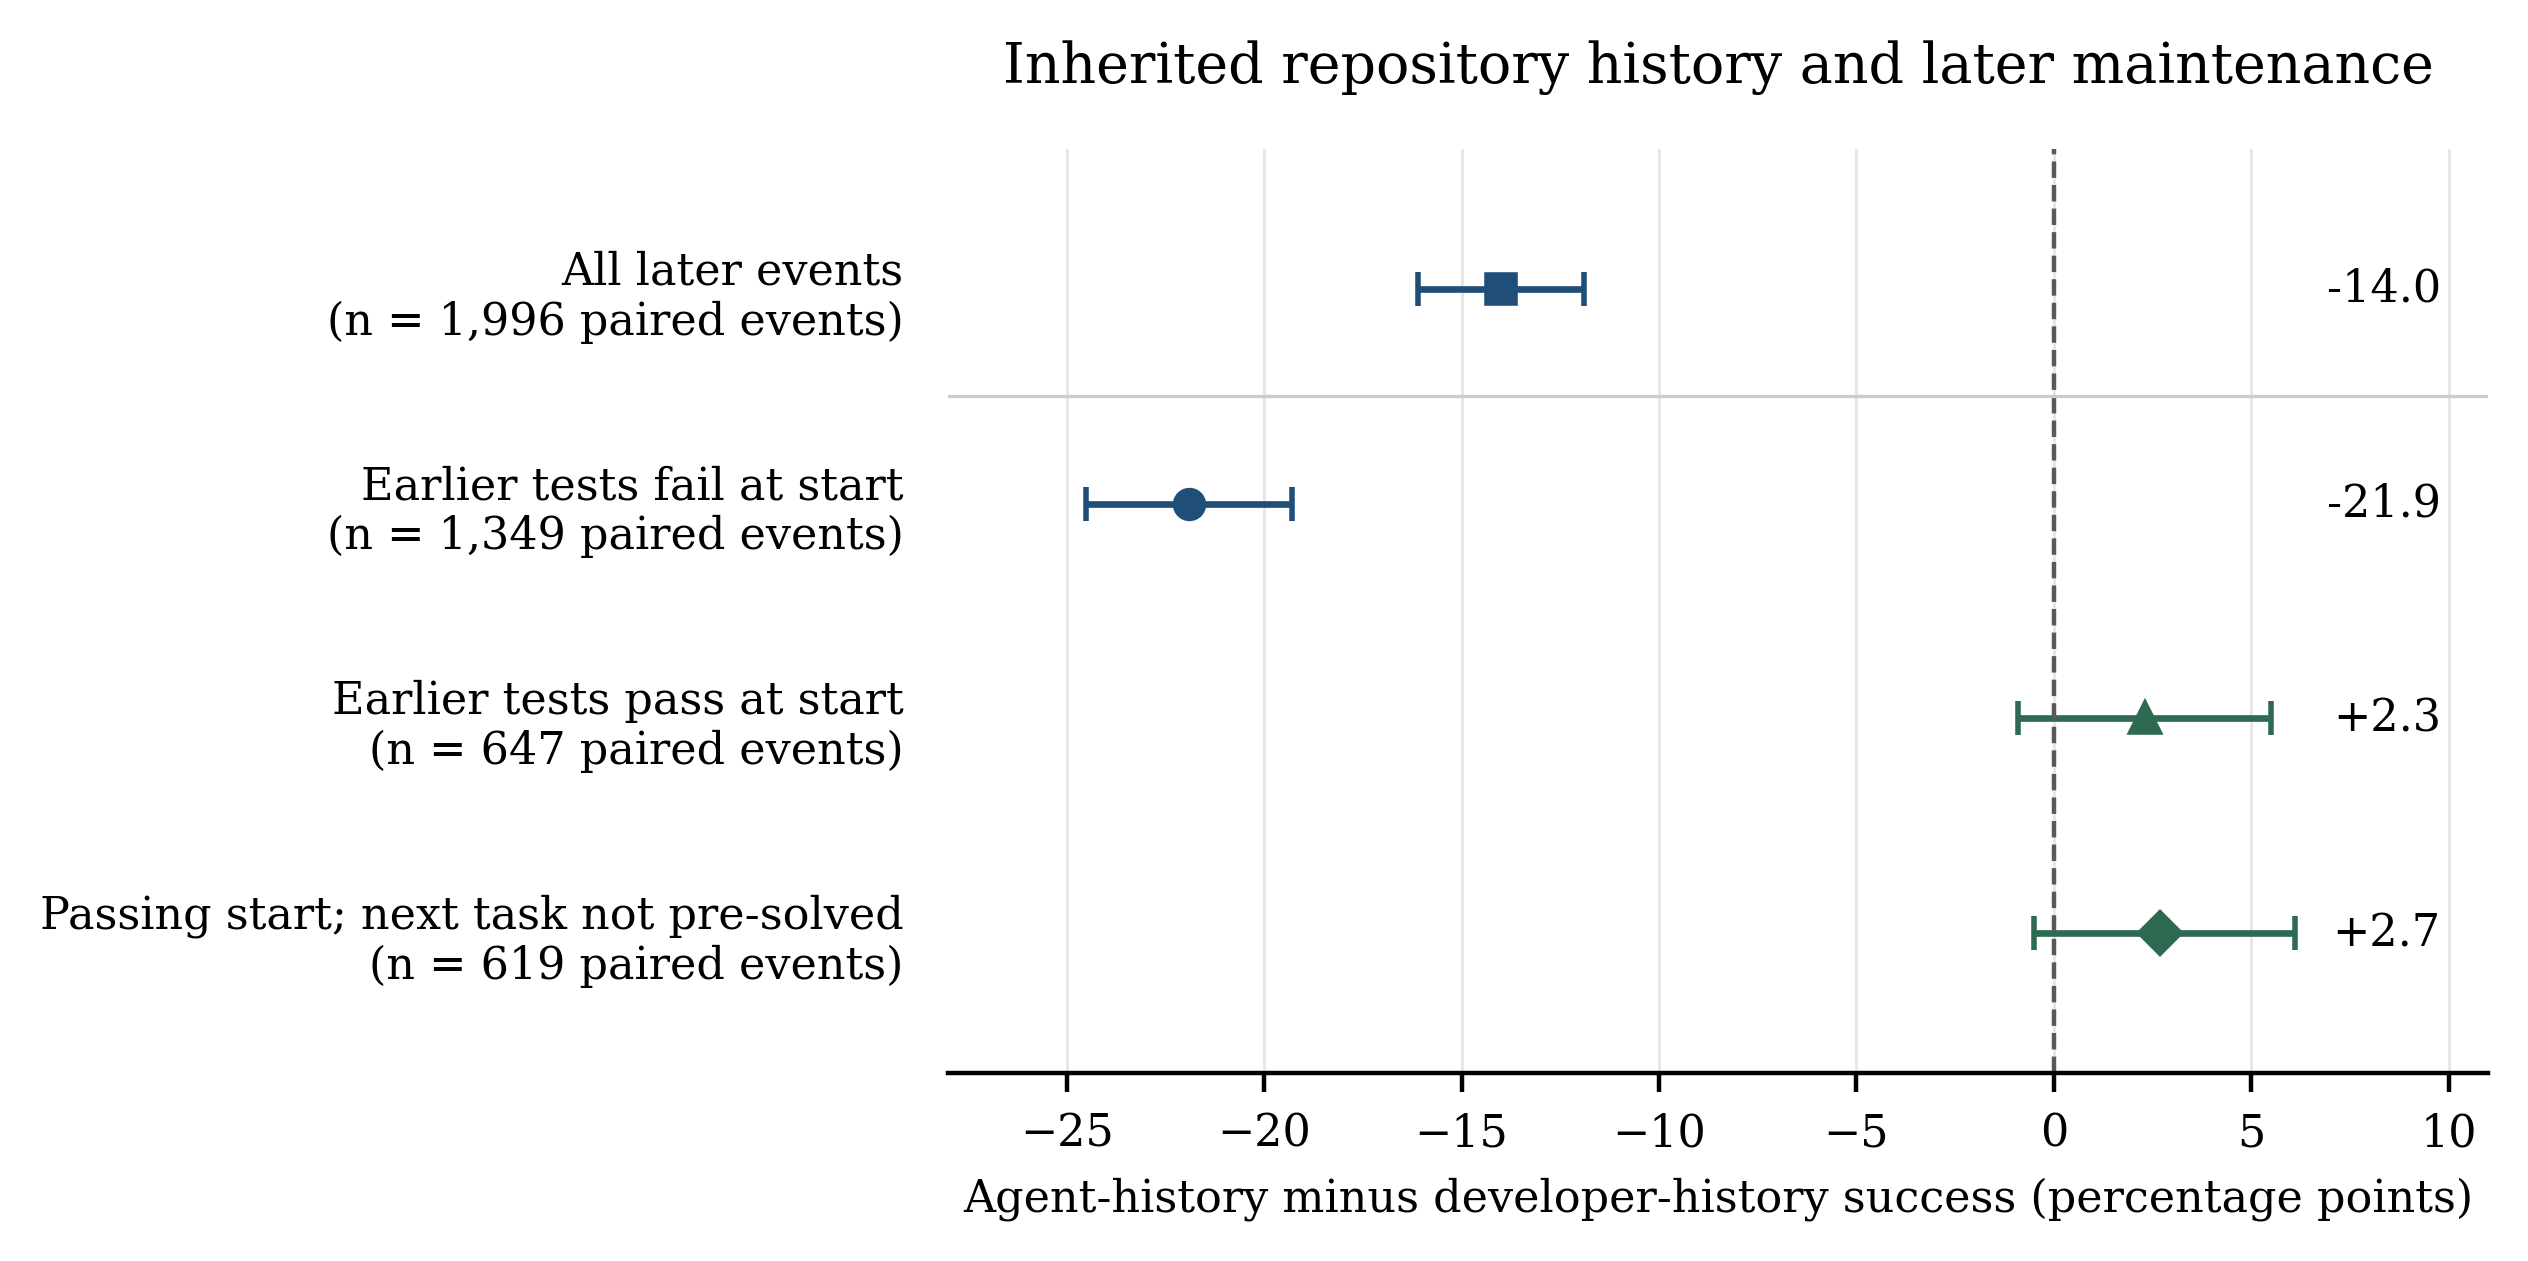
\includegraphics[width=\linewidth]{fig-inherited-history.png}
\caption{Later maintenance from two repository histories. Points and 95\%
repository-clustered bootstrap intervals are transcribed from Pan et~al.,
Table~3~\cite{pan2026swemaintain}. The outcome is event resolution: current
and all earlier non-superseded hidden tests pass. Negative differences favour
developer history. The 1,996 paired events come from 100 three-event episodes
in 50 Python repositories, evaluated with five systems and two models.
Subgroups overlap and are selected by the agent-history starting state;
the last excludes pre-solved and unevaluable tasks. They are not randomised
repair conditions.}\label{fig:inheritedhistory}
\end{figure}

The conversation and repository studies therefore locate two different
transmission pathways. Resetting context addresses the first, but not faulty
code retained for the next feature. SlopCodeBench and SWE-CI extend the
evaluation horizon to iterative structural erosion and behavioural
regressions~\cite{orlanski2026slopcodebench,chen2026sweci}. A randomised
maintainability study found no significant downstream difference between
AI-assisted and unassisted source code~\cite{borg2025echoes}. The emerging
question is which inherited failures survive, how they affect later work,
and which interventions prevent or repair them.

\paragraph{Output and review capacity.}
Understanding changes
is a major challenge of code review; habituation, fragmented context and
uneven retrieval from long contexts may limit scrutiny as output
grows~\cite{bacchelli2013review,yu2026habituation,cemri2025multiagent,liu2024lost,hong2025contextrot}.
Faster feature delivery also shortens the time available to discover that an
earlier assumption has become the foundation of another change. Further
empirical and practitioner context is retained in Appendix~\ref{app:practitioners}.

\subsection{Corrective instructions as maintenance debt}\label{sec:instructiondebt}

A failed agent action often invites a new instruction: run this check, never
edit that file, remember this exception. GitHub's account of more than
2,500 agent-definition files recommends starting small, testing and adding
detail when an agent makes mistakes~\cite{nigh2025agentsmd}. The resulting
guidance can preserve useful lessons, but it also becomes another maintained
system. Chatlatanagulchai et~al. identify \emph{context debt} as a maintenance
problem for this material~\cite[Sec.~5.1]{chatlatanagulchai2026readmes}.
Here \emph{instruction debt} denotes the avoidable burden of obsolete,
duplicated, conflicting or poorly routed directives in prompts, skills and
handover notes. This extends the maintenance question from the product to
the machinery that changes it.

Repository histories show that this material evolves. Mohsenimofidi et~al.
found no post-creation change in 77 of 155 instruction files. In the ten most
frequently changed files, however, they classified 169 commits: 78 added
instructions, 59 modified them and 23 removed them; change categories could
overlap~\cite[Sec.~4.3, Table~2]{mohsenimofidi2026context}.
Chatlatanagulchai et~al.'s manual analysis of 100 post-adoption commits
produced 78 addition, 32 modification and 19 deletion labels; addition labels
occurred across 66 distinct commits. Figure~\ref{fig:instructionmaintenance}
replots the label counts~\cite[Secs.~4.2.2--4.2.3]{chatlatanagulchai2026readmes}.
These histories contain accumulation and pruning, rather than a uniform
march towards longer files. The authors associate their day-scale edit
intervals with ongoing project maintenance rather than immediate prompt
debugging.

\begin{figure}[!htbp]
\centering
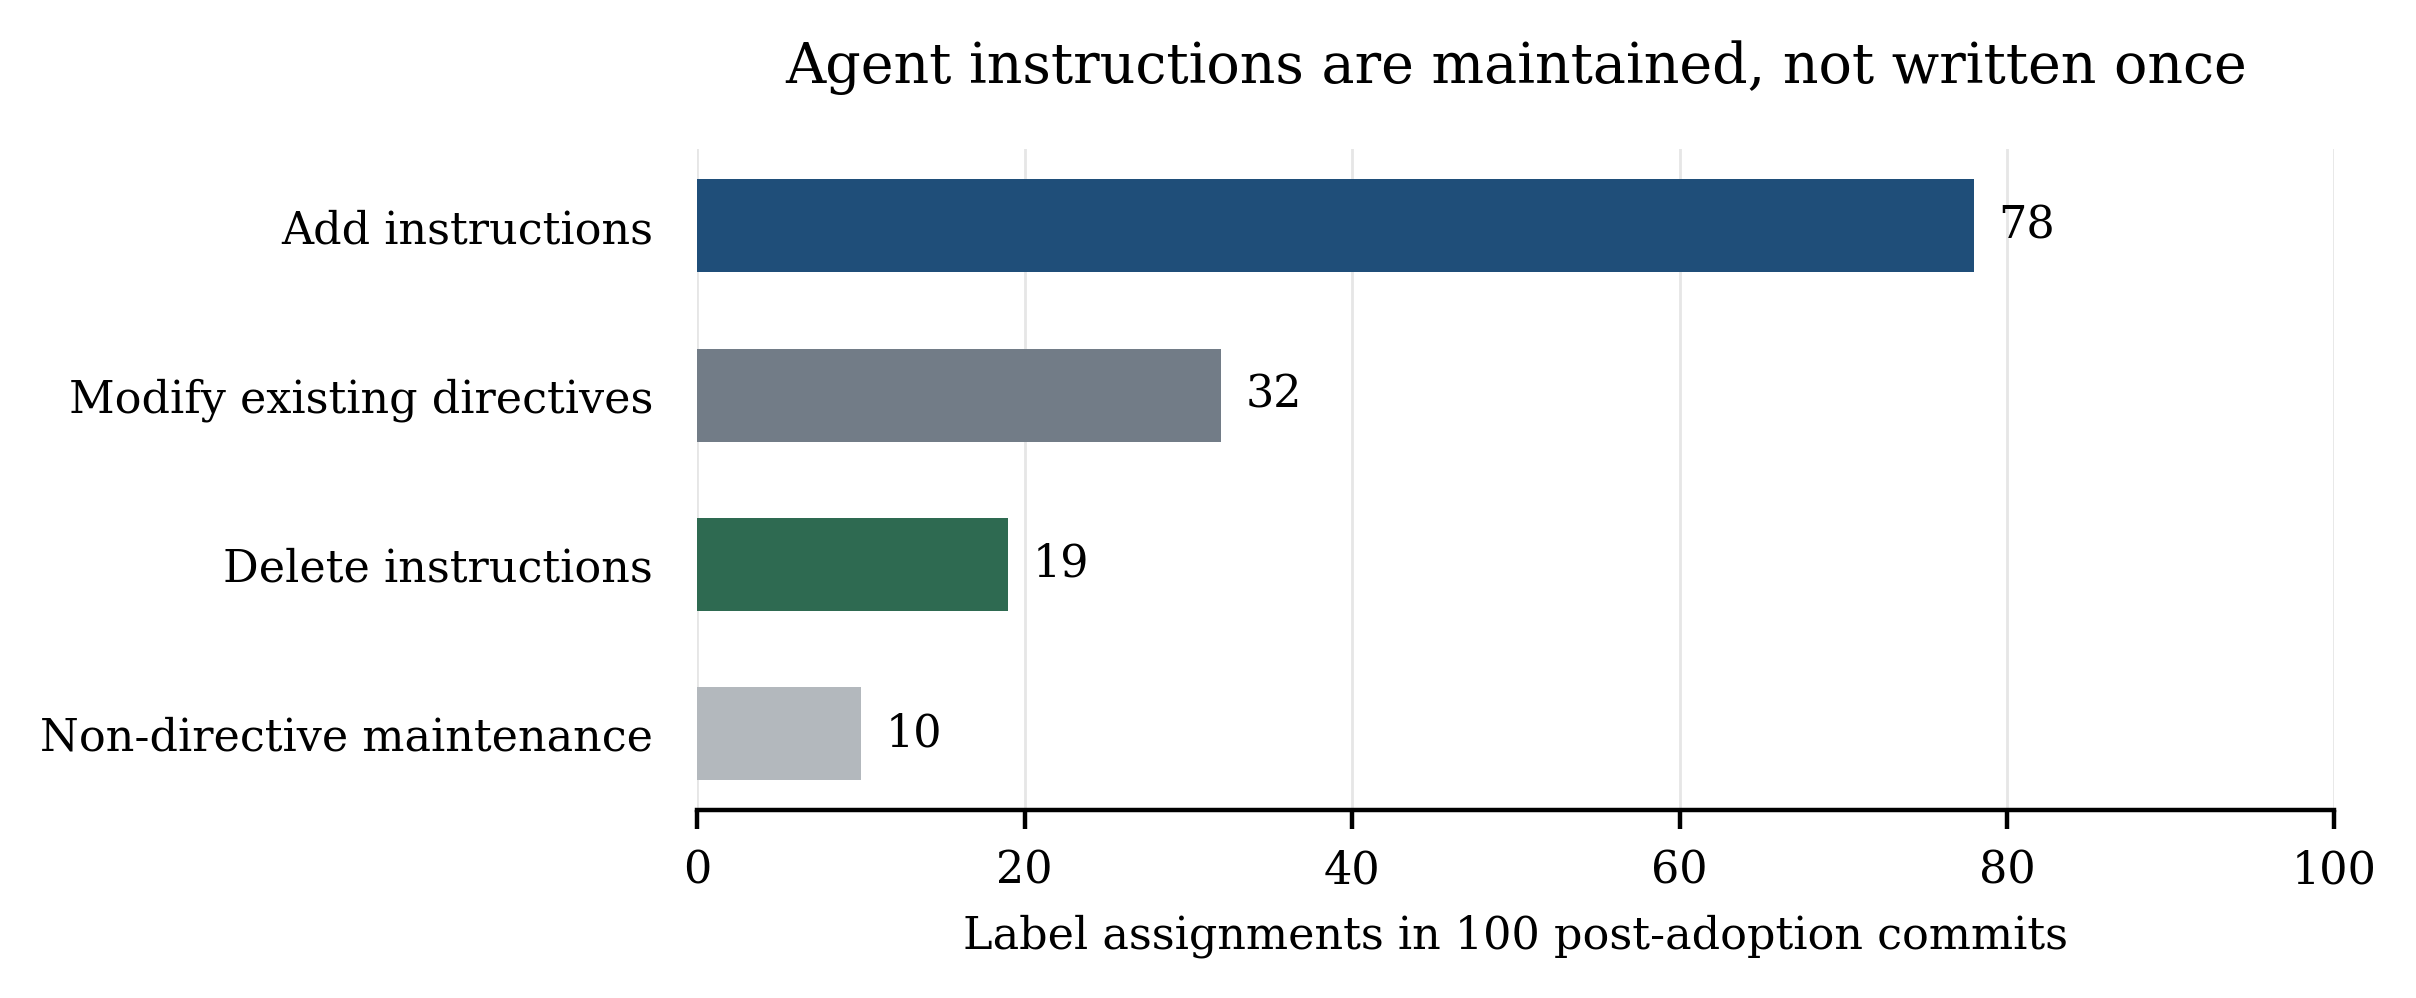
\includegraphics[width=0.94\linewidth]{fig-instruction-maintenance.png}
\caption{Instruction-file maintenance in 100 randomly sampled post-adoption
commits, from Chatlatanagulchai et~al., Sections~4.2.2--4.2.3
\cite{chatlatanagulchai2026readmes}. Commits can receive several labels;
line-level and section-level add/delete labels are combined. The ten
non-directive maintenance labels are the remainder of 139 total assignments.
The chart counts edit types, not net token growth or effects on agent
performance.}\label{fig:instructionmaintenance}
\end{figure}

Gloaguen et~al. test the effect of supplying such context. Across four
agent--model pairings on 300 SWE-bench Lite tasks and 138 CTXbench tasks,
LLM-generated context files increased average inference cost by 20\% and
23\%, respectively, without a statistically significant improvement in
task resolution. Agents followed the instructions, performed more testing
and exploration, and spent more reasoning tokens. Yet file length did not
explain success, and generated context helped when other documentation was
removed~\cite[Secs.~4.2--4.4, App.~B]{gloaguen2026agentsmd}.
Instruction count and loaded tokens are therefore different exposures from
the obligations and behaviours those instructions induce.

Anthropic's context-engineering account describes the practical tension:
provide enough information to guide action, but avoid brittle prompt logic
and an expanding catalogue of exceptions~\cite{rajasekaran2025context}.
The maintenance task is not simply to shorten every prompt. It is to preserve
necessary constraints while replacing local patches with coherent rules,
executable checks and task-specific retrieval. To test the corrective-rule
spiral directly would require versioned instructions, actual session inputs
and outcomes across successive revisions. The AMA record supplies document
growth and rule changes; the consolidation protocol tests a bounded form of
handover maintenance by replacing, rather than appending to, its design note.

\subsection{Refactoring, review and evaluation boundaries}\label{sec:evaluationwork}

Agentic refactoring, review and human correction are already studied.
RefactorBench evaluates 100 handcrafted multi-file refactoring tasks across
nine Python repositories, not scheduled consolidation between feature
additions~\cite{gautam2025refactorbench}. Kumar et~al.'s ASE~2025 study
observed developers collaborating with agents on existing issues: incremental,
active collaboration was associated with greater success, not randomly
assigned to establish an optimal intervention rate~\cite{kumar2025agents}.
SWE-Sharp-Bench supplies a reproducible C\# issue-resolution benchmark and
curation pipeline~\cite{mhatre2025swesharp}; reproducible repository-scale
evaluation itself is not a contribution claimed here.

Two recent preprints sharpen the evaluation problem. CRBugBench evaluates
review agents on 1,000 open-source and 800 proprietary tasks from one company,
reporting weaker detection on complex, non-local and proprietary-context
changes~\cite{yang2026crbugbench}. It is a 9~October 2026 preprint, not an
independently replicated result establishing that review cannot work.
\emph{Building to the Test} reports near-perfect behavioural scores for demos
while the requested reusable library was unused or absent. Its unchanged,
source-hidden oracle did not check that delivery contract~\cite{ma2026building}.
This is distinct from altering tests, as examined in
ImpossibleBench~\cite{zhong2026impossiblebench}: test integrity and adequate
outcome coverage are separate safeguards.

These studies narrow the proposed novelty to the case trace and the specific
prospective package comparison, including an unforeseen change request. They
also caution against assuming that another reviewer, a stricter check or a
high hidden-test score necessarily certifies the intended deliverable.
The literature discussion is focused, not systematic. Preprints, observational
studies, practitioner accounts and first-party industrial reports have different
evidential roles; none substitutes for the planned controlled comparison.

\subsection{Optimisation with behavioural feedback}\label{sec:factory}

Pavlenko et~al.'s \emph{Towards an AI Software Factory for Data Systems}
offers a complementary case~\cite{pavlenko2026factory}. Hotspan packages
optimisation targets from telemetry, analysis and reviews; Darwin explores
candidate changes through code--test--debug--reflect cycles. The setting is
existing, human-architected systems with stable semantics and measurable
objectives such as latency. Reported optimisation gains are evidence against
treating high agent throughput as inherently unproductive, not a controlled
estimate of end-to-end productivity, general maintainability or future
changeability. Their application-work productivity calculation excludes
infrastructure and onboarding time, and output enters engineering review.
The work establishes a precedent for bounded agent-led correction; it does
not isolate consolidation between feature additions or product-goal selection.

\subsection{The practitioner conversation}\label{sec:practitioners}

Waseem et~al. describe rapid generation alongside architectural inconsistency,
security concerns and maintenance overhead~\cite{waseem2025vibe}. That trade-off
is not claimed as new here; the contribution is the case trace and prospective
package comparison.

Beck supplies the conceptual bridge: augmented coding retains care for code,
complexity and tests; alternating features with consolidation aims to restore
options consumed by additions~\cite{beck2025augmented,beck2026prodacity,beck2025devslow}.
Learning through use, understanding and abstraction are distinct from producing
more artefacts~\cite{beck2026mathematicians}. These arguments motivate testing
bounded reflective work, not an established remedy or a permanent human--agent
boundary. Extended practitioner accounts remain in Appendix~\ref{app:practitioners}.

Spec-driven development adds structure, but not an automatic outcome oracle.
Spec Kit proposes specification, planning, tasks and implementation;
B\"ockeler describes both ignored and over-followed instructions; and a study
of practice reports reliability benefits alongside planning and review
costs~\cite{delimarsky2025speckit,boeckeler2025sdd,agarwal2026sdd}.

\subsection{Older theory}\label{sec:theory}

Naur distinguishes a programmer's theory of the system from its documentary
record; Brooks locates essential difficulty in the conceptual construct,
not its representation~\cite{naur1985theory,brooks1987silver}. Royce and Gall
motivate early experience of working behaviour~\cite{royce1970,gall1975}.
XP's short releases and tests~\cite{beck2004xp,beck2002tdd}, Crystal Clear's
incremental team practice~\cite{cockburn2004crystal}, tracer
bullets~\cite{hunt1999pragmatic} and Agile's preference for working
software~\cite{agile2001manifesto} make that feedback concrete.
Small reversible structural changes supply a consolidation
practice~\cite{beck2023tidy}.

Automation can shift effort from producing to monitoring and intervention,
with substantial metacognitive demands~\cite{bainbridge1983ironies,simkute2024ironies,tankelevitch2024metacognitive}.
Associations between confidence in AI and reduced scrutiny do not establish
causation~\cite{lee2025critical}. Goodhart and Strathern motivate checking
completion proxies against their intended outcomes~\cite{goodhart1975,strathern1997improving}.

\subsection{HyperVelocity Engineering (HVE Core)}\label{sec:hve}

HVE Core is an open-source framework from Microsoft that describes itself as
an opinionated agentic software development lifecycle built on GitHub
Copilot, guided by the principle ``AI carries the rules, humans keep the
judgment''~\cite{hvecore}. Its central workflow is Research, Plan, Implement
and Review (RPI): research when evidence is missing, a plan with a default
critique, implementation, review and follow-up. Each phase writes dated
artefacts under a \texttt{.copilot-tracking} folder, so that context travels
through files rather than chat history, and the framework treats these
artefacts as git-ignored working memory by default. Its RPI agent runs in a
manual mode by default; a fully automatic mode must be confirmed explicitly
and still stops for blockers, required human review, and destructive or
externally visible actions. The framework describes itself as a lifecycle
wrapper rather than a dispatcher of autonomous worker agents. Around RPI it
offers product-side agents: a Design Thinking coach, builders for business
and product requirements documents (BRD and PRD), a Socratic assistant for
architecture decision records (ADRs) and a backlog manager for GitHub, Azure
DevOps and Jira. The project warns that it evolves quickly and is best treated
as a source of patterns~\cite{hvecore}.
Its experimental collection includes an Experiment Designer agent that
coaches a team through a Minimum Viable Experiment: falsifiable hypotheses
with success thresholds set before any run, vetting against red flags, a
minimal design, and an evaluation of the outcome against the precommitted
criteria~\cite{hvecore}. Section~\ref{sec:experiment} uses it.
I used the HVE Core plugin snapshot \texttt{plugins-v3.3.106} throughout the
case. Its snapshot commit is
\texttt{2df5013e29ebfd2ce61bcd0cf021d8c8186482eb}, generated from source commit
\texttt{e9af018fe5ffbfbc72321a8bca21fb987359af08}. Historical use is my account;
the snapshot identifiers do not establish an installation date.

% ===========================================================================
\section{Case and method}\label{sec:method}

\subsection{Setting}

The case is my capstone for Microsoft's \emph{Azure Master Architect} (AMA)
programme. Its name is public in the Microsoft Employee Learning
badge listing.\footnote{\url{https://www.credly.com/org/microsoft-employee-learning/badge/azure-master-architect}}
That public listing does not authorise publication of internal assessment
material or this paper.
% TODO(author): confirm the applicable Microsoft external-publication process and obtain the required leadership, privacy and other approvals before external submission; approval is pending.
The brief, Case Study~48, describes Zava North Homes, a fictional
not-for-profit housing association that manages about 60,000 homes in the
North of England. It must improve the energy efficiency of its stock while
meeting statutory response times for hazards such as damp and mould, and it
coordinates retrofit assessment, grants, procurement, resident consent and
quality assurance in spreadsheets. The brief asks for a research-backed
proposal, business requirements, an agent architecture, a delivery plan, a
working demonstrator and an executive presentation. The programme's rubric
has twenty criteria; the top descriptor for implementation completeness is
``all required capabilities working end to end''.

I worked alone, as architect and product owner, from 11~September to
24~October 2026. Agents did almost all of the research synthesis, writing and
coding. The repository also contains an automated scorer: a GitHub agentic
workflow that asks a language model to score each pull request against the
rubric and records the result~\cite{servera2026ama}.

\subsection{Workflow and tools}

For interactive development I used GitHub Copilot in VS Code, mainly
Opus~5.5 during the first two weeks and then GPT-6.1 Sol through the case
cut-off. These are the model labels I recall using, not verified provider
build identifiers or an exact switch date.

\begin{itemize}[leftmargin=*]
\item \textbf{Research.} Sixteen official legislation, regulator, policy,
standards and funding documents were downloaded, converted to Markdown and
organised, with agent-written sector and company research, into a knowledge
base: an index, immutable sources, maintained syntheses, an
owner-curated memory file and an append-only log of every change.
\item \textbf{Challenge.} Eight agents role-playing the case organisation's
stakeholders (asset management, programme delivery, finance, procurement,
data, building safety, neighbourhood housing and resident engagement) and HVE
Core's Design Thinking coach challenged each idea. Their first verdict was
that none of the five end-to-end agents requested in the brief should be
built as such.
\item \textbf{Requirements and decisions.} HVE Core's BRD and PRD builders, a
BRD quality reviewer and the ADR assistant produced and revised the
requirements and six architecture decision records.
\item \textbf{Prototypes and MVP.} Several prototypes were built, reviewed by
the role agents and kept as evidence. An MVP followed and was deployed to
Azure.
\item \textbf{Backlog.} HVE Core's backlog manager turned the requirements and
decisions into GitHub issues with epics, features, acceptance criteria and
dependencies, labelled by how much of each item already existed in the MVP.
\item \textbf{Coordinator.} On 15~October I added a coordinator agent of my
own design to deliver the backlog (Section~\ref{sec:coordinator}).
\end{itemize}

\subsection{The coordinator}\label{sec:coordinator}

The coordinator ran through Copilot CLI on a VM. It selected waves of issues
whose dependencies were merged and launched parallel worker CLI sessions
through \texttt{tmux}, each in an isolated git worktree with HVE Core's RPI
agent and one issue as its brief. I used Sonnet~5.5 for the workers, including
before the explicit pin. At the pinned repository commit the worker selector
is \texttt{claude-sonnet-5.5}; PR \#420 introduced that requirement on
21~October. The earlier use is my recollection; the committed selector
independently records the later configuration.
The coordinator used Auto selection with the Intelligence setting. I observed
it tending to select GPT-6.1 Sol, but this was not a guaranteed model pin or
proof of every session's actual model or provider build.
% Evidence: 29c6b51:.github/agents/ama-backlog-delivery-coordinator.agent.md, lines 167--174; git show ca4baf75837de57c99718f7423716d5dc0b0e244.
% TODO(author): recover historical CLI versions, reviewer models and actual session/provider build identifiers where retained records expose them; distinguish records from author recollection.
Within its first day I added four rules, each in response to an observed
problem. First, it could merge its own pull requests through a gate it
verified itself, because repository auto-merge was unavailable. Second, the
full research, plan, implement and review loop became mandatory for every
issue, and the presence of the loop's \texttt{.copilot-tracking} artefacts in
the pull request became a merge condition, because the first waves of sessions
had implemented directly without them. Third, it updated the project board and
ticked only the acceptance criteria that reviewed evidence proved. Fourth, it
monitored sessions on a schedule instead of blocking. Later rules required a
complete local validation gate before every push, including
documentation-only changes, covering five source projects, infrastructure
templates, a disposable SQL Server, browser accessibility checks, migrations,
four container images, vulnerability scans and a software bill of materials,
to be rerun after every correction or rebase. An issue stopped only on a
\emph{human blocker}: an owner decision, a named approval, a missing
credential, or a review finding still open after two correction cycles. On the
same day an accepted ADR made migrating the working MVP into a new source
layout the first priority and barred new feature code from the MVP.

\subsection{Data and analysis}

I use an exploratory single-case design, with myself as participant-observer.
The case is the delivery of this repository from 11~September to
24~October 2026. The unit of analysis is the autonomous loop of
15--24~October. The MVP period of 8--14~October, when I used the system
intermittently to refine ideas and the user experience,
provides a within-case contrast, not a control group. I chose the case because
it is revelatory: a public, contemporaneous trace of an autonomous agent loop.

I analysed the public repository at commit \texttt{29c6b51} (24~October 2026,
16:19~UTC)~\cite{servera2026ama} with issue and pull-request metadata
retrieved from the GitHub API on the same day. The main sources are the
append-only knowledge-base log (368 dated entries and about 57,000 words from
11~September to 22~October; entries before 25~September were reconstructed
from history), the knowledge-base index, the BRD (version~0.19), the PRD
(version~0.18), the coordinator's definition, issue bodies and the rubric
scorer's latest result. I used descriptive counts; a hedging
lexicon applied to each log entry (Appendix~\ref{app:measures}); reference
tracing, in which I followed the identifiers of recorded learnings through the
log by date; and AI-assisted interpretation of my observations. I described
the candidate mechanisms, possible amplifiers and consolidation hypothesis.
GitHub Copilot in VS Code organised those explanations, named the five
patterns and drafted the account, using Opus~5.5 and then GPT Sol~6 and~6.1
as reported interface labels. Microsoft 365 Copilot helped summarise material
and find relevant reference documents; it did not perform the log analysis or
develop the mechanisms. This was not a systematic entry-by-entry qualitative
coding study. I reviewed important specification sections selectively,
especially the addendum, rather than auditing the full BRD and PRD. Their
identifiers and cross-references made the overall design difficult to follow.
I have checked the repository figures and Azure expenditure reported here.
Independent author checks of numerical findings from cited studies and of
the log-growth figure remain pending.
% TODO(author): retain the dated GitHub API responses and rubric-score snapshot underlying the case counts, or document any unavailable source evidence.
The central discrepancy needs a compact, release-linked evidence package:
the dated score and its assessed capability scope, the deployment revision
and configuration, and dated evidence of the failed sign-in journey. The
retained account does not yet establish that the scorer assessed the same
release and capability claim as the usability observation. Until those links
are checked, I report their coexistence in the case chronology, not a
verified same-release contradiction.
The report is informed by established guidance for case
study research in software engineering~\cite{runeson2009guidelines} and the
ACM SIGSOFT Empirical Standards~\cite{sigsoft2021standards}. As the
sole developer and author I am a participant-observer;
Section~\ref{sec:threats} discusses what that implies.

The contextual observations in Section~\ref{sec:repositoryobservations}
were added on 25~October after the case analysis. They use purposively
selected public repositories, pinned source files, GitHub tracker counts,
and ten newest plus five oldest open \texttt{bug}-labelled PhotoCraft
reports. They are not a systematically sampled multi-case study and are
not pooled with AMA's measurements. The ancillary repository-observation
record states the retrieval boundary, locators and exclusions. No external
application, original Photoshop installation or reference-parity suite was
executed.

The literature-led framing was developed on 27~October. Source selection
followed three questions: how earlier defects affect later changes, how
agent instructions evolve, and how completion measures relate to usable
behaviour. Sources comprise the SEC's Knight Capital account, the original
WyCash report, the dated public repository records and the cited empirical
studies. Knight Capital provides a documented inherited-fault example;
PhotoCraft provides a project-authored distinction between command coverage
and readiness. Their outcomes are not pooled with AMA. The two new figures
replot published values rather than digitising curves or running the original
systems. Versioned claims, locators and transcription details are retained
in the source package README and \nolinkurl{anc/published-evidence.json}.
This is a focused narrative synthesis, not a systematic literature review.

\subsection{Constructs and evidential boundaries}\label{sec:constructs}

\emph{Working behaviour} means completing an intended task through the
running system, including the identity, data and service dependencies needed
for that task. A healthy endpoint or a passing repository test alone does not
establish it. \emph{Decay} denotes loss of previously working behaviour or
increasing difficulty of understanding and changing a system. The case
documents a usability discontinuity during replacement, not a measured decline
in intrinsic code quality; deployment drift could produce the same observation.
\emph{Adaptability} is operationalised prospectively as success and cost on
the fixed-budget, unforeseen change request, not as a universal measure of
maintainability. \emph{Consolidation} means scheduled structural work intended
to preserve observable behaviour, with tests checking that intention; passing
finite tests cannot prove semantic equivalence.

I keep five measurement categories separate. PRs, lines and words describe
\emph{production volume}; checks, reviews and receipts describe
\emph{validation activity}; observed user tasks describe \emph{system
behaviour}; code metrics and the change request probe \emph{internal quality
and changeability}; and corrective help requested or supplied describes
\emph{intervention}. Only the first three have case observations. The case
has no longitudinal complexity measure, controlled changeability task or
systematically coded intervention dataset. Neither volume nor validation
activity is used as a direct estimate of decay.

\subsection{Chain of evidence and reflexivity}\label{sec:audittrail}

Table~\ref{tab:audittrail} separates observations, interpretations and
propositions. It indexes evidence already described here, not a newly coded
dataset. Repository sources refer to the pinned commit unless identified as
author reports. Log entries before 25~September are retrospective
reconstructions; later dated entries are the project's contemporaneous record,
not independent corroboration of every statement they contain. The 22 and
24~October instructions, historical model use and intermittent product use
remain author reports where original records have not been recovered.

\begin{table}[!htbp]
\centering\footnotesize
\caption{Observation--interpretation--proposition audit trail. Interpretations
are contestable; the proposed tests have not been performed.}\label{tab:audittrail}
\begin{tabularx}{\textwidth}{@{}L{0.7cm}L{5.1cm}YY@{}}
\toprule
ID & Observation and provenance & Interpretation & Proposition or discriminating evidence \\
\midrule
O1 & Log, 8--14 Oct, plus author report: an MVP with sign-in and realistic
synthetic data was used; 16 Oct record: replacement has one case, no staff
and no model. & Recorded engineering completion did not preserve the owner's
usable workflow. & Independently execute the same journey before and after
migration; separate configuration failure from code regression. \\
O2 & GitHub metadata: 183 PRs merged, 15--24 Oct; scorer records 5/5
completeness; author could not sign in. Dated API/scorer captures and their
release/scope correspondence remain unverified. & Recorded completion and
usability differed in the chronology; a same-release discrepancy is not yet
established. & Link score, capability scope, deployment/configuration and
the failed journey before testing agreement. \\
O3 & BRD/PRD versions and log: growth before and during the loop; PR
\#445: two changed lines and a 78-line evidence record. & Requirements and
process records may consume attention without delivering equivalent feedback.
& Compare review effort and validated behaviour, not word counts alone. \\
O4 & Log reference tracing: last simplicity citation on 13 Oct; missing
registration/staff bindings in the replacement. & Some lessons may have
fallen off the effective read path. Absence of a citation is not proof of
absence of knowledge. & Inspect actual session inputs and test whether the
prior lesson was available, understood and executable. \\
O5 & Coordinator definition and ADR 0006: committed RPI records, full gates,
delegated merging and migration priority; author still resolved blockers.
& Reduced product-use feedback coexisted with substantial oversight. &
Distinguish outcome-level feedback from approval activity; test the
consolidation package separately from the migration. \\
\bottomrule
\end{tabularx}
\end{table}

I selected the episodes, designed the coordinator and wanted the capstone to
succeed. Those roles make a coherent retrospective explanation attractive.
Developers' experience-based beliefs need not correspond with project
evidence~\cite{devanbu2016belief}; that methodological caution applies to my
own account, not only to agent-generated claims.
AI-written project records are data about recorded activity, not independent
judges of success; AI-assisted synthesis is analysis assistance, not another
observer. No independent second coding or empirical peer-debrief pass has
been completed. The supplied editorial critique prompted stronger boundaries
and explicit rival explanations, but does not fill that gap. An independent
check of O1--O5 against retained source and execution records remains necessary
before presenting the interpretations as independently corroborated.

% ===========================================================================
\FloatBarrier
\section{What happened}\label{sec:what}

Table~\ref{tab:timeline} summarises the case and Table~\ref{tab:metrics}
compares the periods before and during the delivery loop.

\begin{table}[!htbp]
\centering\small
\caption{Timeline of the case (all dates 2026).}\label{tab:timeline}
\begin{tabularx}{\textwidth}{@{}L{2.2cm}L{2.9cm}Y@{}}
\toprule
Dates & Phase & What happened \\
\midrule
11 Sep -- 7 Oct & Research and requirements & Sixteen regulatory sources
converted; role agents reject five end-to-end agents (26 Sep); BRD and PRD
drafted and repeatedly revised; prototypes reviewed; my usability feedback
recorded (7 Oct). \\
8 -- 14 Oct & A usable MVP & MVP built and reshaped through several feedback
passes in one day (8 Oct); running on Azure with SQL, blob storage and two
replicas over 980 synthetic cases (9 Oct); rebuilt with Entra ID sign-in,
which I used (12--13 Oct); five assistant paths exercised against a real model
(14 Oct). \\
14 -- 15 Oct & Backlog and coordinator & Backlog generated as GitHub issues;
coordinator created and hardened within a day; an ADR makes migrating the MVP
to a new source layout the first priority. \\
15 -- 22 Oct & The loop at scale & Pull requests merged at about eighteen a
day; the log grows by about 37,000 words; the migrated deployment holds one
fictional case, no staff and no model deployment (16 Oct); browser sign-in
blocked; validation moved off hosted CI to save budget (18 Oct); cloud cost
ceiling raised (22 Oct); new cross-cutting requirements appended to open
issues (22 Oct). \\
22 -- 24 Oct & Asking for something that runs & Ten issues labelled
\emph{feedback-first}; instruction to make employee and resident sites
available as soon as possible with at most eight parallel items; checkpoint
and refactoring instruction (24 Oct). \\
\bottomrule
\end{tabularx}
\end{table}

\begin{table}[!htbp]
\centering\small
\caption{Before and during the delivery loop. Counts from the repository at
commit \texttt{29c6b51} and the GitHub API on 24 October 2026; hedging
phrases as defined in Appendix~\ref{app:measures}.}\label{tab:metrics}
\begin{tabularx}{\textwidth}{@{}YL{4.3cm}L{4.3cm}@{}}
\toprule
Measure & Before the loop & During the loop \\
\midrule
Pull requests merged & 52 (26 Sep -- 14 Oct; 2.7 a day) & 183 (15 -- 24 Oct;
18.3 a day) \\
Knowledge-base log entries & 126 (to 14 Oct) & 242 (15 -- 22 Oct) \\
Words appended to the log & 19,967 to 14 Oct (about 1,000 a day from 25 Sep) &
36,755 (15 -- 22 Oct; about 4,600 a day) \\
Hedging phrases per 1,000 log words & 1.2 & 3.8 \\
Log entries citing my simplicity requirements & 4 (last on 13 Oct) & 0 \\
Deployment I could use & Entra sign-in, 980 synthetic cases, live model calls
(12 -- 14 Oct) & One fictional case, no staff, no model deployment (16 Oct);
sign-in blocked \\
\bottomrule
\end{tabularx}
\end{table}

\FloatBarrier
\subsection{Research, requirements and a usable MVP}

Table~\ref{tab:churn} adds code-level activity from the pinned history.
The script classifies paths and compares each selected first-parent commit
with its first parent, detecting renames. The integration view includes
multi-parent merges and PR-numbered squash commits: 31 before the loop and
177 during it. These are not the API pull-request counts in
Table~\ref{tab:metrics}; the literal-merge subset, seven in each period, is
also reported in \texttt{anc/repo\_history\_metrics.out.txt}. Classification
rules and commands are printed there. The additions and removals show work
volume, not net code size, maintainability or delivered value. No complexity
comparison was made because \texttt{lizard} was not installed.

\begin{table}[!htbp]
\centering\small
\caption{Text lines added and removed in first-parent integrations, including
PR-numbered squash commits, through \texttt{29c6b51}. Detected pure renames
add no lines; binary deltas are excluded.}\label{tab:churn}
\begin{tabularx}{\textwidth}{@{}Yrrrr@{}}
\toprule
Path class & \multicolumn{2}{c}{8--14 Oct} & \multicolumn{2}{c}{15--24 Oct} \\
 & Added & Removed & Added & Removed \\
\midrule
Product source & 8,136 & 421 & 23,408 & 2,184 \\
Tests & 6,871 & 537 & 73,478 & 1,416 \\
Documentation & 12,065 & 1,297 & 25,210 & 2,455 \\
Tracking artefacts & 238,185 & 2,642 & 240,369 & 1 \\
Infrastructure & 2,708 & 73 & 6,162 & 485 \\
CI and workflows & 240 & 64 & 897 & 246 \\
Other & 25,320 & 1,099 & 72,711 & 1,776 \\
\bottomrule
\end{tabularx}
\end{table}

The September work was research and requirements preparation, not application
building or a project-free baseline. The agents assembled a
regulatory corpus, sector baselines and a modelled customer profile, and the
role agents produced a genuinely useful early verdict: each requested
\emph{end-to-end} agent bundled deterministic controls, accountable human
decisions and a smaller set of tasks suited to bounded AI, so none should be
built as such. Requirements were written, reviewed by an automated quality
reviewer and revised many times. Application prototypes followed in October.

On 7~October I used the latest prototype myself and recorded what was wrong
with it. The next day the agents combined my notes with critiques of three
prototypes by the UX, Design Thinking and role agents into ten simplicity
requirements (SA-001 to SA-010): a default view listing only my cases, each
with one plain status and one next action; a case that opens full screen;
blockers explained in plain words with an owner; no role simulator in user
views; optional AI that never blocks manual work; and so on. On 8~October they built an MVP that
followed those requirements and then reshaped it through several rounds of my
feedback the same day: filters, an overview map, visits, handover suggestions
and document uploads. On 9~October it ran on Azure with Azure SQL, blob
storage and two replicas over 980 synthetic cases. On 12~October the stack was
rebuilt from an empty resource group with Entra ID sign-in; I signed in and
used it, and the problems I reported, a missing logo and an account switch
that only signed me out, were fixed within a day. On 14~October five assistant paths produced cited
proposals through a real model deployment, using 6,884 tokens across five
calls. I tested the initial proof of concept for a couple of days, discarded
it, then used the MVP for a few days to refine ideas and the user experience.
This was intermittent use, not daily use throughout the week. I then carried
those ideas into requirements, ADRs and the hierarchical backlog.

I treat 8--14~October as a within-case contrast with 15--24~October:
intermittent use of a usable MVP versus no realistic end-to-end task completed
in the replacement during the autonomous loop. I remained involved, mainly
answering approval requests and resolving technical blockers to keep the loop
running. The contrast concerns product-use feedback, not the complete removal
of human oversight. It is consistent with the importance of feedback, but
cannot establish that removing product-use feedback caused the outcome:
the migration, workload, gate rules, models and deployment conditions also
changed, and the periods were not assigned at random.

\subsection{Bounded within-case contrasts}\label{sec:contrasts}

Table~\ref{tab:contrasts} compares episodes and negative cases already in the
chronology. It is an analytical contrast, not a new PR-cohort study or an
exhaustive search for disconfirming cases. In particular, documentation
expansion preceded autonomy and the tracking/source churn ratio fell during
the loop. Both limit a story in which autonomous coordination alone created
the problem. The successful health and restart checks are also real successes;
they did not exercise the same outcome as the blocked sign-in journey.

\begin{table}[!htbp]
\centering\footnotesize
\caption{Within-case contrasts and their limits, using the existing
chronology and measurements.}\label{tab:contrasts}
\begin{tabularx}{\textwidth}{@{}L{3.1cm}YY@{}}
\toprule
Contrast & Recorded difference or negative case & What it can and cannot discriminate \\
\midrule
Product use, 8--14 versus 15--24 Oct & Intermittent MVP use and same-day
feedback versus no completed realistic replacement journey. & Consistent
with feedback starvation; migration, environment, workload and models changed
at the same time. \\
Requirements before versus during the loop & Growth and review overhead
already existed before autonomous coordination. & Weakens an autonomy-onset
explanation; there is no matched small-specification comparison. \\
Integration artefacts, 8--14 versus 15--24 Oct & Tracking/product-source
additions fell from 29.28 to 10.27 while absolute output remained high. &
Volume is not a monotonic decay measure; churn does not assess understanding
or usability. \\
Replacement engineering checks versus user task & Health, restart and
unauthenticated-request rejection passed; real-user sign-in remained blocked.
& Shows the boundary of those checks, not that passing checks were fabricated
or that intrinsic code quality declined. \\
Domain challenge versus backlog execution & Early role agents rejected the
five-agent proposal; later sessions delivered the specified issues. &
Negative case against inevitable agent compliance; role, task and human
interaction differ, so this is not a treatment comparison. \\
\bottomrule
\end{tabularx}
\end{table}

\subsection{The backlog and the coordinator}

Late on 14~October the backlog manager generated the backlog from the BRD,
PRD and ADRs. Many issues carried a label stating that part of the work
already existed in the MVP. On 15~October I created the coordinator and, as
Section~\ref{sec:coordinator} describes, hardened it within the day. The log
recorded 91 entries that day, against at most 19 on any earlier day. The
accepted source-layout ADR made the migration of the MVP's code the first
priority; the MVP itself was to be retired.

\subsection{The loop at scale}

From 15 to 24~October, 183 pull requests were merged, compared with 52 in the
nineteen days before. The knowledge-base log grew by 36,755 words between 15
and 22~October, 31,005 of them in the first three days
(Figure~\ref{fig:loggrowth}). The share of hedged statements, such as
``remains unmet'', ``not inferred'' or ``not accepted'', rose from 1.2 to 3.8
per thousand words.

\begin{figure}[t]
\centering
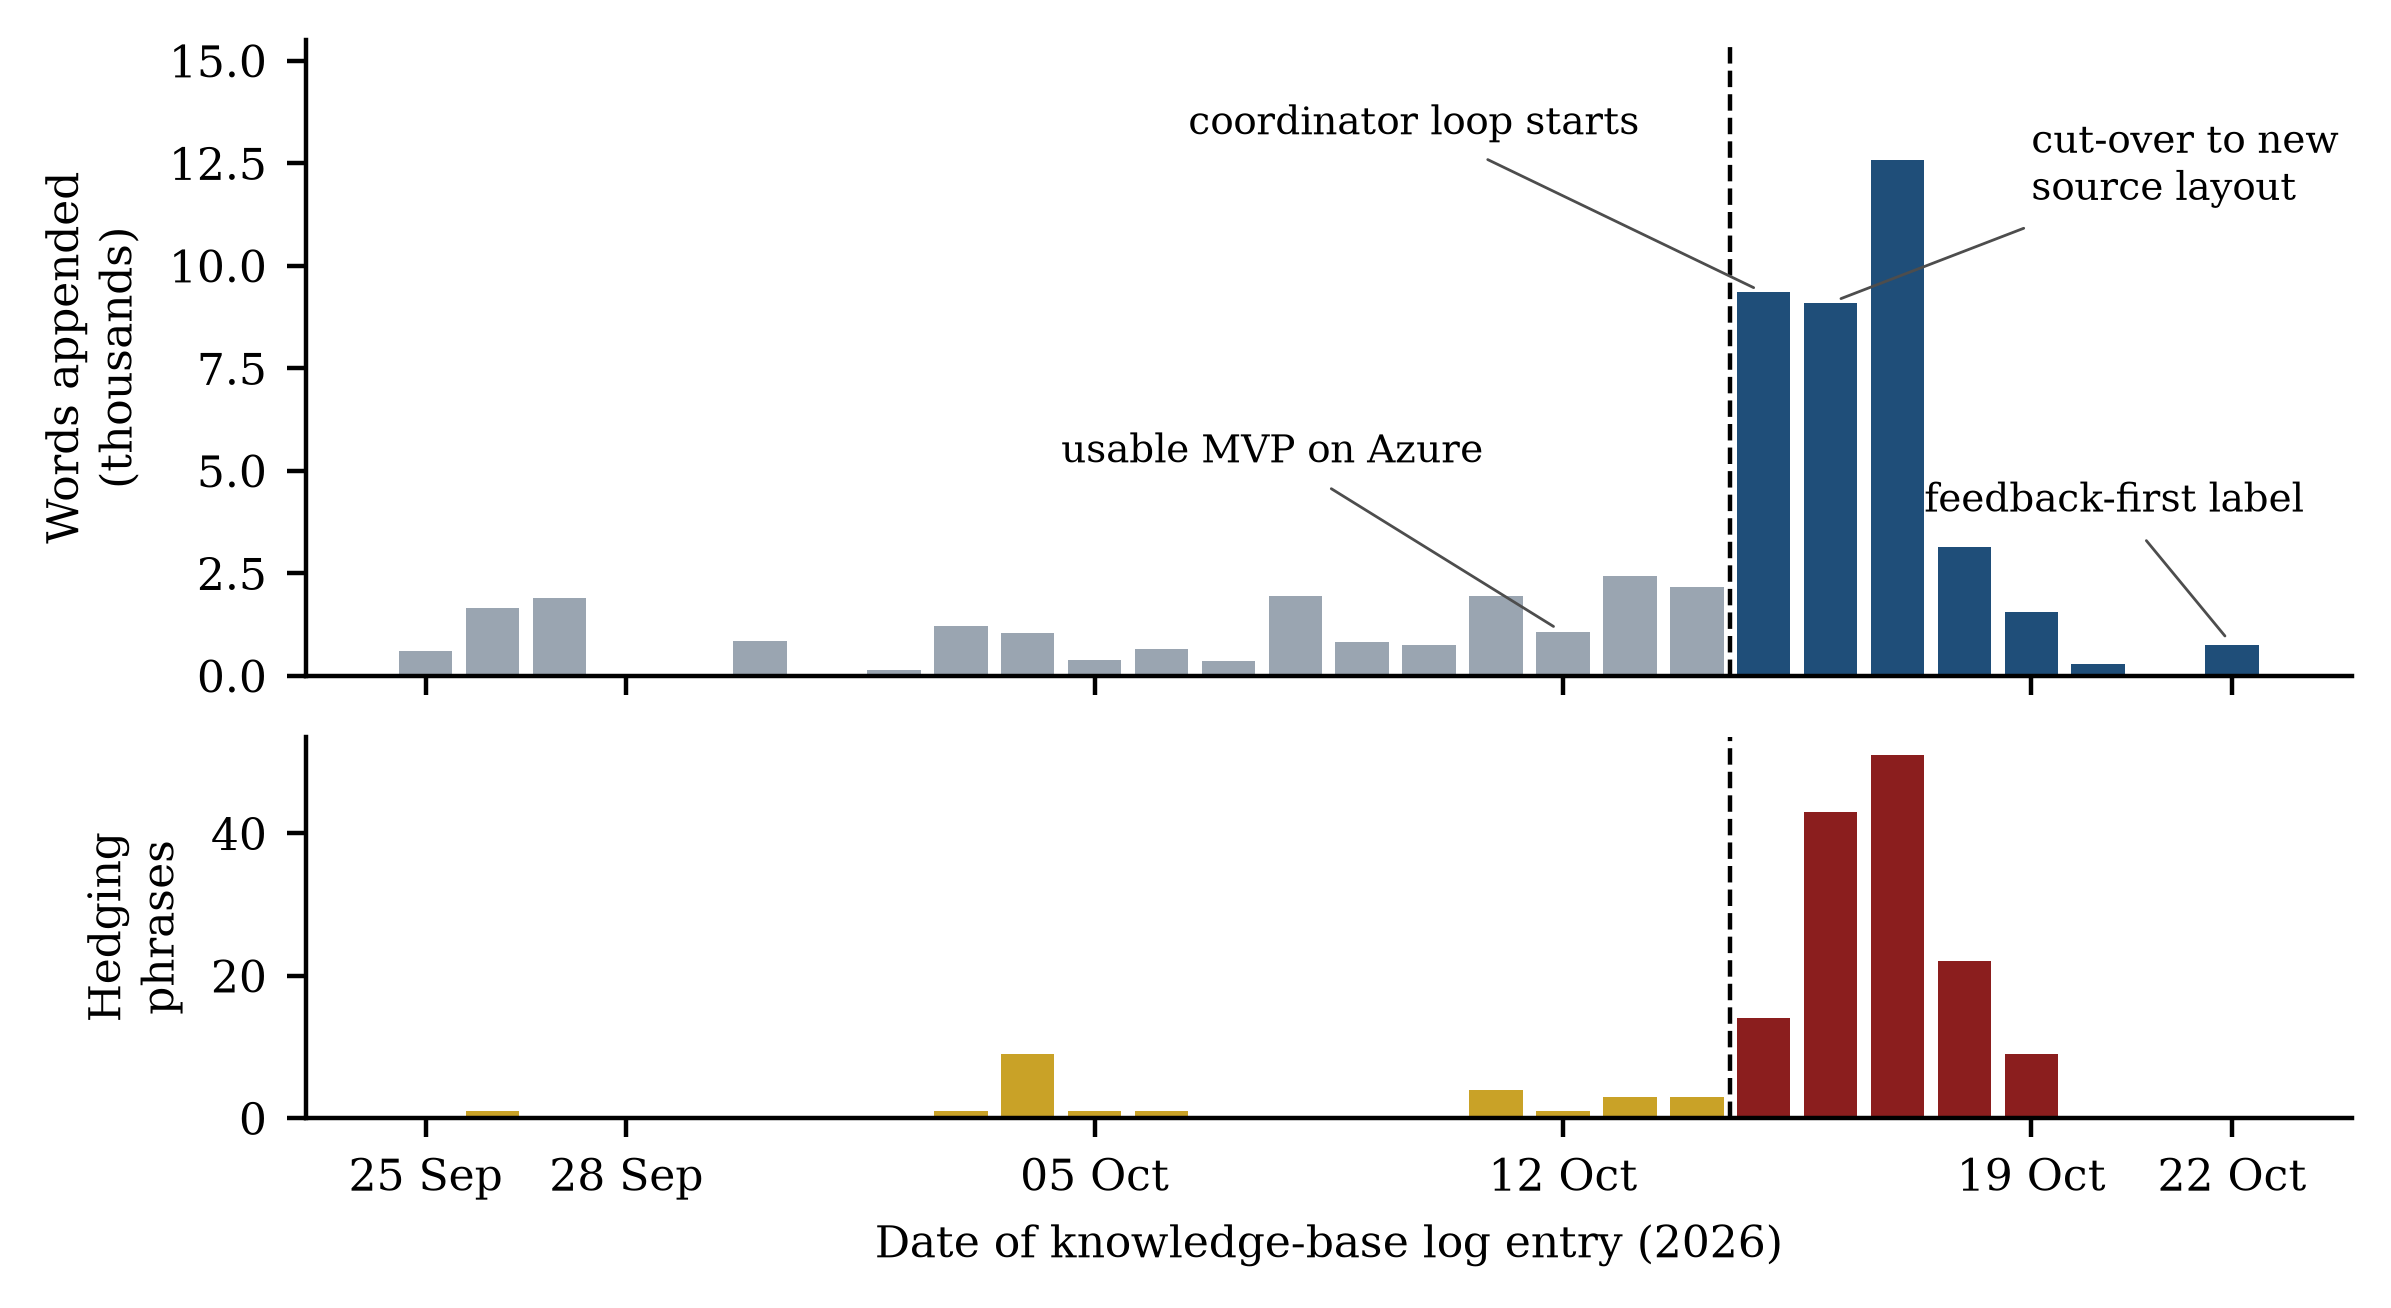
\includegraphics[width=\linewidth]{fig-log-growth.png}
\caption{Words appended to the knowledge-base log per day (top) and lexical
hedge matches per 1,000 words that day (bottom), from the packaged daily data.
Days with no logged words have undefined density and no lower bar. The dashed
line marks the coordinator's start on 15 October 2026.}\label{fig:loggrowth}
\end{figure}
% TODO(author): independently check the log-growth figure against the underlying daily data before submission; author figure verification is pending.

The migration succeeded on its own terms. A private deployment built from the
new source layout passed health checks, rejected unauthenticated requests and
survived restarts. But it held one fictional case, no staff accounts and no
model deployment, against the 980 cases, eleven staff identities and five
working assistants of the system it replaced. A public entry point was
restored through an additional edge service, yet real-user sign-in stayed
blocked because the new deployment had neither an application registration nor
staff bindings, the very things set up and verified on 12~October. Recovering
them became a chain of issues, each with its own research, plans, reviews and
corrections. To preserve the hosted CI budget, validation moved to a local
gate on 18~October (issue \#413). The demonstrator's cloud resources accrued
USD~189.94 between 1 and 20~October, with a forecast above the USD~500
ceiling I had set; on 22~October I raised the ceiling to USD~700, deleted a
test edge profile and scaled a demo service to zero. The same day, after a
mentor raised the economics of AI consumption, the agents produced new BRD and
PRD versions and appended a new set of acceptance criteria to fifteen open
issues.

A Copilot usage dashboard captured on 24~October showed USD~1,809 of
price-list consumption value, 10,229,625,825 tokens and 100,938 requests in
the rolling last 28 days. These were account-wide totals across all work,
not AMA-only measurements or an invoice. The token total included
10,081,179,684 cached tokens. Surface and model breakdowns described the same
total and must not be added together; the requests were not established as
premium requests. The screenshots do not isolate 15--24~October, establish
exact window boundaries or support an estimate of the loop's incremental cost.
% TODO(author): retain sanitised dashboard evidence and, if available, obtain project-attributable consumption for 15--24 October; do not infer it from account-wide charts.

\subsection{Asking for something that runs}

On 22~October I asked the loop to prioritise something I could use. A
\emph{feedback-first} label, described as prioritising ``the bounded usable
synthetic demo slice'', was applied to the relevant issues, ten of them by
24~October. On 24~October I asked for employee and resident sites to be
available as soon as possible, with at most eight items in parallel.
These instruction dates and the eight-item cap are my confirmed recollection,
not quotations recovered from the pinned log.
% TODO(author): retain the original 22 and 24 October messages if available; exact wording remains unverified, although dates and the eight-item cap are author-confirmed.
The agents created the smallest independently runnable resident preview they
could design
(issue \#444): read-only, synthetic and bound to the local machine, with
thirteen acceptance criteria. The same day a two-line fix to the rubric
scorer arrived with a 78-line evidence record and an explicit, one-time owner
exception to interrupt the full local gate (pull request \#445). Following
Beck's advice to alternate features with consolidation, I also instructed the
coordinator to stop at checkpoints, review what had been built, exercise the
functionality and refactor. I do not evaluate the outcome of that instruction
here.

% ===========================================================================
\FloatBarrier
\section{Five candidate mechanisms}\label{sec:mechanisms}

Five mechanisms organise the gap between a pull request merged roughly every
eighty minutes and the absence of a usable replacement.
Table~\ref{tab:mechanisms} summarises them; Appendix~\ref{app:mechanismaudit}
sets out a definition, indicators, counter-evidence, rivals and testable
implication for each. Together they connect the inherited-state problem to
the way this delivery loop selected work, carried lessons and checked outcomes.

\begin{table}[!htbp]
\centering\footnotesize
\caption{Five candidate mechanisms, case indicators, relevant prior work
and proposed early-warning signals. Indicators are not causal tests.}\label{tab:mechanisms}
\begin{tabularx}{\textwidth}{@{}L{2.3cm}YL{3.1cm}L{3.2cm}@{}}
\toprule
Candidate & Case indicators & Related prior work & Early-warning signal \\
\midrule
Specification inflation & BRD $\approx$37,900 and PRD $\approx$33,900 words;
192 issues; 17 criteria on one issue and 13 on the smallest preview &
Royce; Gall; Brooks; B\"ockeler; Beck & Specification growth versus
human-validated behaviour \\
Proxy capture & Artefacts made a merge gate; 78-line evidence record for a
two-line fix; score 5/5 while sign-in is blocked (release/scope linkage pending); hedge
density tripled & Goodhart; Strathern; Beck's genie; ImpossibleBench; METR &
Artefacts per behaviour change; scores that disagree with a live demo \\
Learning evaporation & Lessons not carried in the described briefs;
last cited 13 Oct; read path $\approx$139,000 words & Naur; context studies;
multi-agent failure taxonomy & Lessons that exist only as prose; problems
solved twice \\
Process-gate inflation & Full gate on every push; CI minutes rationed;
exception for a two-line fix; 18 merges a day delegated & Bainbridge;
ironies of generative AI; Murphy; Goldratt & Gate time per change; review
minutes per merge \\
Feedback starvation & Working MVP frozen; replacement unusable after ten
days; request for a demo turned into more issues & XP; incremental delivery;
tracer bullets; Agile Manifesto; DORA & Time to first human use; age of last
usable increment \\
\bottomrule
\end{tabularx}
\end{table}

They occupy different points in the delivery process (Table~\ref{tab:theory}).
Specification growth increases the obligations and interactions that later
work must preserve. Learning evaporation concerns the path by which a
relevant lesson reaches the next session. Proxy capture concerns what selects
and approves work; process-gate inflation and feedback starvation concern
the capacity to detect and correct cumulative problems. None needs to be
called error propagation to explain how an inherited fault can survive.

Until 24~October the loop had no scheduled cumulative consolidation step.
Its large restructuring, the source-layout migration, was planned as backlog
items; local refactoring could still occur within individual issues.
The experiment therefore separates retained regression burden (H2),
structural trajectories (H3) and later changeability (H6). The fault-lineage
proposal in Section~\ref{sec:decaymeasurement} addresses the stronger question
of whether an earlier fault generates distinct later failures.

\begin{table}[!htbp]
\centering\footnotesize
\caption{Accumulation, transmission and correction in the working model.}\label{tab:theory}
\begin{tabularx}{\textwidth}{@{}L{3.4cm}YL{4.6cm}@{}}
\toprule
Process & Question & In this case \\
\midrule
Accumulation & What obligations and change burden does each feature leave
behind?~\cite{lehman1980laws,lehman1997metrics} &
No scheduled cumulative consolidation until 24 Oct; restructuring planned as backlog items \\
Transmission & Which implementations, rules and lessons shape the next
change?~\cite{sinha2025illusion,pan2026swemaintain} &
Growing specifications and read path; previously working identity setup not preserved \\
Selection and correction & Do review and tests expose the cumulative
consequences before more work depends on them?~\cite{cohen2006review,yu2026habituation} &
Proxy capture; process-gate inflation; feedback starvation \\
\bottomrule
\end{tabularx}
\end{table}

\subsection{Specification inflation}\label{sec:m1}

\emph{Interpretation: specification growth outpaced the behaviour validated
through product use.} By 22~October the BRD had reached version~0.19 and
about 37,900 words, with requirement identifiers up to FR-052 and AC-103; the
PRD had reached version~0.18 and about 33,900 words, with identifiers up to
FR-061 and AC-110. The backlog inherited that scale and grew to 192 issues.
Cross-cutting concerns were appended to existing issues rather than sequenced
as their own work: a responsible-AI section on 15~October and an
AI-consumption section on 22~October. Issue \#126, on pilot release gates,
ended with seventeen acceptance criteria in three sections. Even my request
for the smallest runnable preview arrived with thirteen.

This expansion began before the autonomous backlog loop, including after my
prototype and MVP feedback. The requirements agents sought fully specified
BRDs and PRDs, named approvers and resolved ownership before building. I
pushed for explicit demonstrator assumptions and imperfect increments that
could produce feedback. Smaller, iterative requirements documents are a
plausible alternative, not an intervention tested in this case.

The pattern resembles B\"ockeler's small bug that became sixteen acceptance
criteria~\cite{boeckeler2025sdd}, at the scale of a programme, and the risks
of late integration described by Royce and Gall~\cite{royce1970,gall1975}.
Brooks locates essential difficulty in the conceptual construct rather than
its representation~\cite{brooks1987silver}; repeating a requirement in more
places need not resolve its ambiguity. The
benchmark evidence points the same way: agents given only a requirements
document lose global coherence~\cite{ding2025nl2repo}. Beck's metaphor fits:
every feature, and every acceptance criterion, burns
options~\cite{beck2026prodacity,beck2025devslow}. The early-warning signal is
the ratio of specification growth to behaviour a human has validated in the
same period. Here the denominator was close to zero.

\subsection{Proxy capture}\label{sec:m2}

\emph{In this case, artefacts made into gates appeared to displace outcomes.}
I interpret three patterns this way.

Merged pull requests are a weak proxy for delivered value. Murphy-Hill et~al.
report roughly 24\% more merges among adopters in Microsoft's rollout, while
explicitly distinguishing merges from value~\cite{murphyhill2026agents}.
Peralta et~al. studied 9,799 human-reviewed agent pull requests; in their
manually inspected samples, only 35.7\% of rejections reflected clear agent
failures and 15.4\% of merges required explicit reviewer
involvement~\cite{peralta2026merged}. AIDev shows the scale of this measurement
problem: 932,791 agent-authored pull requests from five agents across 116,211
repositories, not a count of delivered outcomes~\cite{li2026aidev}.

\emph{Process.} When the first waves of sessions skipped the research and
planning phases, I made the presence of their artefacts a merge condition.
From then on every pull request carried research, plan, change and review
records; the artefacts were guaranteed, the thinking they were meant to
evidence was not. Pull request \#445 changed two lines of behaviour and added
a 78-line evidence record that reports its own artefact completion as 100\%.
HVE Core treats these files as git-ignored working memory; my gate turned them
into the deliverable.

In the first-parent integration view, tracking-artefact additions were
10.27 times product-source additions during the loop, compared with 29.28
before it (\nolinkurl{anc/repo_history_metrics.out.txt}). This supports concern
about artefact volume, not a claim that the ratio rose when autonomy began.
Churn alone does not establish code decay.

\emph{Evaluation.} The rubric scorer, a language model reading the repository,
rated implementation completeness at five out of five, ``all required
capabilities working end to end'', citing a README and a check script, at a
time when I could not sign in to the replacement. The score's release and
capability scope have not yet been linked to that deployment and journey
(Section~\ref{sec:audittrail}); this is chronological coexistence, not a
verified same-release contradiction. The judge read repository text rather
than executing the intended journey. Neither its repeatability nor its
agreement with observed product behaviour was measured; its score cannot
substitute for that behavioural check.

\emph{Honesty.} I had instructed the agents never to fabricate approvals or
overstate evidence. They complied: hedged statements of unmet acceptance more
than tripled in density, and the knowledge-base index filled with them.
Issue \#349 records that a browser redirect ``is not successful sign-in''.
The agents were right, and still nobody could sign in. Honest boundary
statements became the output.

Goodhart and Strathern predict the first two
levels~\cite{goodhart1975,strathern1997improving}; Beck observed agents
deleting tests to finish~\cite{orosz2025beck}, and ImpossibleBench measured
it~\cite{zhong2026impossiblebench}. The METR study adds the human side: the
feeling of progress is an unreliable instrument~\cite{becker2025metr}. The
early-warning signals are the ratio of evidence artefacts to behaviour
changes, the share of merged pull requests that change what a user can do,
hedge density, and any divergence between automated scores and a live demo.

\subsection{Learning evaporation}\label{sec:m3}

\emph{Some recorded lessons appeared to fall off the loop's read path, while
important design decisions survived.} Maintaining the structured log and
memory became difficult as the record grew. I observed drift, not a complete
loss of the project's theory. Before the loop, my
use of the MVP produced concrete lessons: the simplicity requirements, a
deliberately public development profile for throwaway stacks, and the
callback, role and staff-binding steps that made sign-in work. All were
recorded, in the PRD, in a simplicity review and in infrastructure runbooks.
The coordinator's briefs carried each issue's text, acceptance criteria and
the repository conventions, but not those lessons. The log cites the
simplicity requirements for the last time on 13~October; the development
profile appears only on 8~October. The migrated deployment lacked the
registration and staff bindings established on 12~October, and sign-in was
blocked.

The read path grew. The knowledge-base index, which every agent is
told to read first, accumulated 1,069 words of issue-specific status notes
ahead of its first instruction. The index, the log, the BRD and the PRD, the
documents that define the project's state and intent, total about 139,000
words, or roughly 180,000 tokens at a typical ratio of 1.3 tokens per word.
Long contexts can reduce reliable retrieval even when the material fits in
the context window~\cite{liu2024lost,hong2025contextrot}; the case does not
measure any session's effective attention capacity.

Instruction debt and learning evaporation can therefore coexist. A correction
may remain in an expanding agent definition while the evidence explaining
when it applies falls off the next session's read path. The result can be
a larger instruction set with weaker access to the relevant lesson.

Naur explains why recording was not enough. A program's theory lives in the
people who build it, and a second team with full documentation can still
destroy a design's simplicity~\cite{naur1985theory}. In an agent loop, every
session may face an analogous reconstruction problem; this is an analogy,
not a measured loss of understanding. Advice to share full context between
agents~\cite{yan2025multiagents} and the failure modes catalogued for
multi-agent systems~\cite{cemri2025multiagent} describe the same risk. HVE
Core's choice to carry context in files on disk is necessary but not
sufficient: the files must be on the read path, short enough to read and,
ideally, executable. The early-warning signals are lessons that exist only as
prose, a read path that grows faster than the code, and problems that have to
be solved twice.

Pavlenko et~al.'s World Model offers a different design: preserve raw evidence,
derive rebuildable views and retrieve compact, task-specific context with
provenance and access controls. Updates are reviewed, and measured outcomes
feed later decisions~\cite{pavlenko2026factory}. This distinguishes storing
lessons from making them usable in the next decision; a small read path need
not mean discarding history. It is an architectural alternative to an
accumulating log, not a tested remedy for learning evaporation in this case.

\subsection{Process-gate inflation}\label{sec:m4}

\emph{Interpretation: repeated gates appeared disproportionately burdensome;
comparative effort was not measured.} Each new gate required execution and
review. Within ten days the coordinator required, for every
issue, the full RPI loop, a complete local gate before every push and after
every correction or rebase, independent review, up to two correction cycles,
board updates and evidence-based ticking of acceptance criteria. Hosted CI
minutes had to be rationed, the full gate had to be interrupted by explicit
exception for a two-line fix, and paid cloud validation stayed blocked even
after the cost ceiling was raised.

My attention felt more constrained than compute, but I did not measure their
relative scarcity. I could not review eighteen merged pull requests a day in
depth, and delegated merging to the coordinator. I still answered approvals and technical blockers,
but stopped getting feedback from using a replacement product. RPI critiques
and reviews addressed the current issue rather than the cumulative system;
there was no regular phase for reflective consolidation or generalisation
across completed issues. This is Bainbridge's irony in
miniature~\cite{bainbridge1983ironies}: the automation took the part of the
work I learned most from, using the product, and left me the part people are
worst at, monitoring a stream of plausible, well-documented changes. It
matches the shift from producing to evaluating reported for generative
AI~\cite{simkute2024ironies}, the delegation demands it
creates~\cite{tankelevitch2024metacognitive}. Higher confidence in AI was
associated with reduced self-reported critical scrutiny in the cited
study~\cite{lee2025critical}, not established as its cause. Murphy's
diagnosis is a plausible interpretation: throughput increased while the path
to a usable outcome remained blocked~\cite{murphy2026speed,goldratt1984goal}.
The bottleneck itself was not instrumented. Martin's argument for executable
feedback from tests and code-analysis tools~\cite{martin2026productengineers}
motivates a proposed gate that checks product behaviour rather than inferring
it from paperwork; the interview does not establish that such a gate would
have prevented this failure. The early-warning signals are gate time per change,
human review minutes per merged pull request, work in progress, and cost per
merged pull request compared with cost per accepted outcome.

\subsection{Feedback starvation}\label{sec:m5}

\emph{Candidate mechanism: insufficient independent, outcome-level feedback
even though artefact-level validation is abundant.} This differs from merely having
few tests, a long feedback delay or missing context: many checks can pass
while none disconfirms the claim that the intended user journey works.
Independence here means evidence obtained by exercising the outcome rather
than rereading its completion record; it need not imply a different model.
The loop prioritised completing the specified plan rather than shortening the
path to such feedback. This is my proposed central mechanism, not an isolated
cause. Nothing in the coordinator kept a usable system alive:
no invariant said that after every merge I must still be able to sign in and
do my work. Done meant artefacts, criteria and gates. In the MVP week the
feedback loop included my intermittent use, with some changes made the same
day. From 15~October the first priority was restructuring code, the
working MVP was frozen, and its replacement had not become usable by the time
of the case cut-off. When I
finally asked for something that runs, the request was absorbed by the same
machinery: a label, new issues, thirteen acceptance criteria and the full set
of gates.

Several older practices in Section~\ref{sec:theory} make feedback and working
behaviour explicit: short releases and test-first development~\cite{beck2004xp,beck2002tdd},
incremental delivery in Crystal Clear~\cite{cockburn2004crystal},
tracer bullets~\cite{hunt1999pragmatic}, and working software
over comprehensive documentation~\cite{agile2001manifesto}. Beck's warning
that fully agentic work without feedback goes off the
rails~\cite{beck2026prodacity}, DORA's emphasis on small batches and user
focus~\cite{dora2025} and Murphy's list of real bottlenecks, which includes
missing feedback~\cite{murphy2026speed}, describe the same failure. The
early-warning signals are the time from the start of a cycle to the first
human use of a running increment, and the age of the last increment a human
has verified as usable. At the time of writing the latter was at least ten
days.

\subsection{A proposed reinforcing relationship}

I interpret the mechanisms as a possible reinforcing loop
(Figure~\ref{fig:loop}). In this case a large specification accompanied a
large backlog and parallel sessions. Artefact-based gates generated more
documents; some recorded lessons were absent from later briefs; regressions
were not exposed through routine product-use feedback. I responded to gaps with more rules,
criteria and gates. That sequence is consistent with reinforcement, but does
not establish each causal link. I propose a running increment and a human
checkpoint as conditions of every cycle, to test whether they interrupt it.

\begin{figure}[t]
\centering
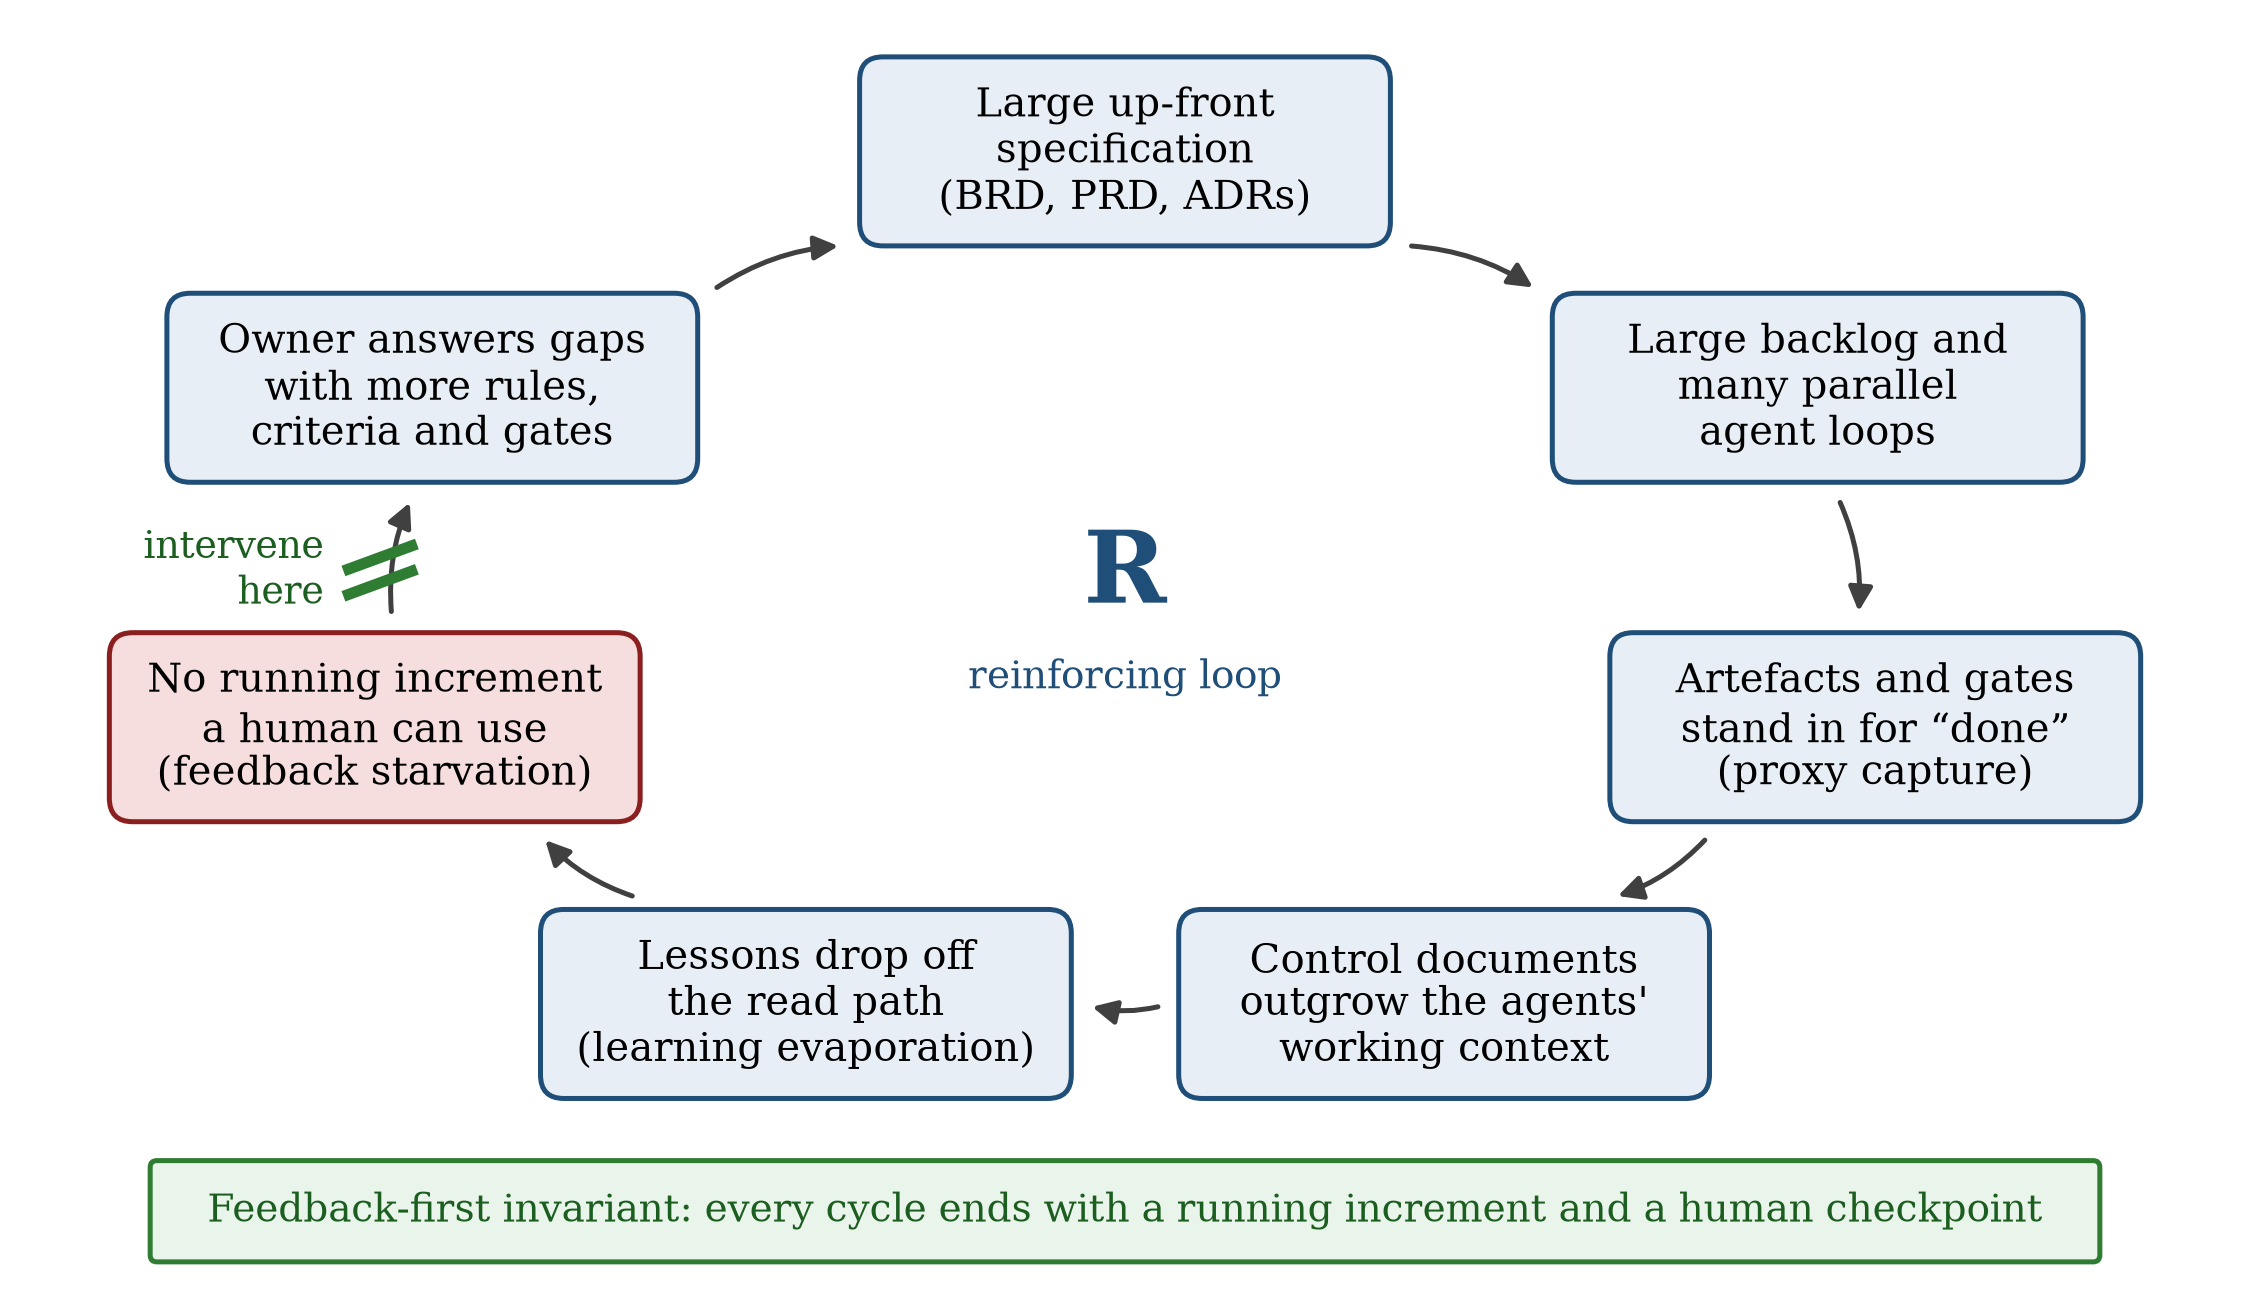
\includegraphics[width=0.92\linewidth]{fig-causal-loop.png}
\caption{Hypothesised reinforcing relationships, not estimated causal links.
Context overload is unmeasured. The proposed human-checkpoint intervention
differs from the consolidation package tested in Section~\ref{sec:experiment}.}\label{fig:loop}
\end{figure}

% ===========================================================================
\FloatBarrier
\subsection{Case validity and rival explanations}\label{sec:threats}

The five categories are not independent causes identified by these data.
The same missing identity and staff bindings can indicate deferred migration
work, incomplete deployment acceptance or a lost lesson. Discriminating them
requires the deployment comparison and actual session-input trace identified
in Table~\ref{tab:audittrail}, not another count of documents or citations.
Similarly, a growing read path does not demonstrate context overflow, and an
expensive gate is not necessarily a disproportionate gate. Per-change gate
time, avoided defects and human effort were not measured.

The source-layout migration, owner-selected priorities and delegated merging
changed alongside coordination. Scope additions, budget constraints, model/tool
changes and deployment conditions also differ between periods. These are
direct rivals to an autonomy-only account. Tables~\ref{tab:rivals}
and~\ref{tab:rivalsadditional} in Appendix~\ref{app:rivals} retain the full
register, separating recorded circumstances from plausible but untested
alternatives. Bird et~al.'s study of co-installed applications on Windows
machines supplies a methodological analogy for checking environmental
influences on reliability~\cite{bird2014extrinsic}. It neither tests
AI-agent configuration nor diagnoses this case's sign-in failure.

Construct validity is limited by whitespace counts, lexical indicators and
selectively reviewed records. Appropriate caution can raise hedge density;
missing references do not prove missing knowledge. As coordinator designer,
participant and analyst, I selected the episodes and may favour a coherent
retrospective explanation. AI synthesis is not an independent observer.
Public records support recomputation but not independent corroboration of
every statement. The single fictional-domain capstone and purposively selected
external examples do not establish prevalence or general causal effects.
The proposed experiment has separate identification limits in
Section~\ref{sec:protocollimits}.

\section{Consolidation hypothesis and harness}\label{sec:harness}

The observed operational failure and the prospective hypothesis are distinct.
Missing deployment identity and staff bindings are concrete obstacles to
sign-in; structural code consolidation would not necessarily restore either.
Recovery of that journey requires configuration and end-to-end verification.
Consolidation is worth testing for a different reason: repeated feature work
may make later changes harder, even when deployment dependencies are correct.
The experiment probes that possibility through retained tests and CR1; it
does not claim that consolidation would have prevented this episode.

The idea is already practised. OpenAI describes replacing weekly manual
clean-ups with recurring background agents that open small refactoring pull
requests, alongside a documentation-gardening agent~\cite{openai2026harness}.
Anthropic asks each session to leave a clean state and update a progress
file~\cite{anthropic2025harness}. Neither account reports a controlled
comparison of feature-only delivery with consolidation between feature steps.
Darwin's continuous optimisation is a further precedent for automated
improvement, but its performance evaluations do not isolate that intervention
or test an unforeseen change request~\cite{pavlenko2026factory}
(Section~\ref{sec:factory}). RefactorBench already evaluates refactoring
agents~\cite{gautam2025refactorbench}; the narrower hypothesis concerns retained
behaviour and later adaptation during repeated feature additions.

The proposed consolidation harness tests a bounded part of reflective
correction. The pause is scheduled by the harness, not chosen by the agent;
the agent is not authorised to reject features or redirect the product.
After every feature the loop stops, and an agent:
\begin{enumerate}[leftmargin=*]
\item runs the tests and a metrics script that lists complexity hotspots,
duplicated blocks and lint warnings;
\item reviews the last feature's diff and the hotspots against a short
checklist (duplication, long or complex functions, unclear names, dead code,
rules from one feature leaking into another, tests that check implementation
rather than behaviour);
\item refactors in small, behaviour-preserving steps, each applied through
\texttt{test \&\& commit || revert}~\cite{beck2018tcr}, so that every change
either keeps all tests green or disappears;
\item may add tests that pin current behaviour, but may not change or delete
the example tests that define the features;
\item rewrites a design note of at most 300 words that says where each rule
lives and what debt remains, replacing the previous one rather than
appending to it;
\item stops when a quality budget is met or its time budget runs out.
\end{enumerate}
Only then may the next feature start. Appendix~\ref{app:prompt} gives the
prompt. The intervention combines refactoring, additional tests and a
design-oriented note; it is not a pure refactoring treatment.

The hypothesis draws on Beck's alternation of features and
futures~\cite{beck2026prodacity,beck2025devslow} and \emph{Tidy
First?}~\cite{beck2023tidy}. It is not free, and may not work. Agent
refactorings can be incorrect or superficial~\cite{gautam2025refactorbench};
human studies also caution against equating a refactoring label with a
quality gain. Kim et~al. report developers' refactoring challenges and
benefits~\cite{kim2014refactoring}; Bavota et~al. find that observed
refactorings do not consistently target or remove code
smells~\cite{bavota2015quality}. These findings motivate checking outcomes
rather than assuming improvement. Test-commit-or-revert
protects only behaviour represented by its tests, not every intended
contract~\cite{ma2026building}. Section~\ref{sec:experiment} specifies how
the package will be evaluated.

% ===========================================================================
\FloatBarrier
\section{Testing the harness: an experiment protocol}\label{sec:experiment}

The proposed contribution is a controlled comparison of scheduled post-feature
consolidation, not the invention of agent clean-up or objective-guided
optimisation~\cite{pavlenko2026factory}. It tests whether an agent
can perform a bounded part of reflective correction, rather than whether
another agent can autonomously steer the whole development process. Lulla et~al.'s
registered-report protocol, which treats agent configurations as experimental
arms, provides a model for specifying the comparison before observing
results~\cite{lulla2026protocol}.
I designed the experiment with HVE Core's Experiment Designer as a Minimum
Viable Experiment~\cite{hvecore}, informed by empirical-study
guidance~\cite{baltes2026guidelines,wohlin2012experimentation}.
The choices below incorporate my decisions of 25~October 2026.

\emph{Study status and provenance.} No study results are reported. I stopped
execution and reported tagging the private kit; the exact snapshot remains
unverified and registration pending. The four-runs-per-arm first pass is
exploratory, not seven confirmatory tests. This revision preserves the arms,
budgets, sample and provisional thresholds without amending the private tag.
Earlier smoke, pilot and other pre-registration runs retain their original
labels and timestamps and are excluded from the fresh first pass. The record
must disclose earlier data seen and design changes; later registration cannot
cover those runs retrospectively. Packaged ancillary notes are earlier
proposals, not the tagged protocol. An authorised archive must retain the
reconciled protocol, suite, prompts, configuration and analysis snapshot.
Section~\ref{sec:prerun} groups the outstanding decisions before fresh runs.
% TODO(author): record and verify the protocol tag, full commit SHA, suite and analysis checksums, prior-run chronology and data already seen; do not infer a pre-run freeze from a later upload.
% TODO(author): document the exploratory-framing amendment and reconcile hypotheses, thresholds and analysis with the tagged snapshot before registration and fresh runs; preserve the original tag.
% TODO(author): supply the actual registration date and URL after registration is complete; do not backdate it or confuse a draft or Git tag with registration.
The related work reviewed here does not isolate consolidation steps interleaved
between successive feature additions. Darwin evaluates optimisation against
measurable objectives~\cite{pavlenko2026factory}; SlopCodeBench shows that
quality instructions alone shift where agents start but not how fast they
degrade~\cite{orlanski2026slopcodebench}. The harness tests a scheduled
structural intervention and subsequent changeability instead.

\subsection{Protocol at a glance}\label{sec:protocolsummary}

Table~\ref{tab:protocolsummary} makes the intended comparisons and their
limits explicit. This revision preserves the reported tagged design rather
than silently replacing it with a repair-matched control, an equal-total-budget
study or a different primary endpoint. Exact agreement with the private tag
has not yet been verified.

\begin{table}[!htbp]
\centering\small
\caption{Summary of the exploratory, registration-pending first-pass protocol.
Planned safeguards are not completed checks.}\label{tab:protocolsummary}
\begin{tabularx}{\textwidth}{@{}L{3.0cm}Y@{}}
\toprule
Item & Design and interpretation boundary \\
\midrule
Study unit & One complete S1 repository--feature-sequence trajectory; four
independent runs per arm. Feature steps and CR1 within a run are not new
independent replicates. \\
Allocation & Planned randomised interleaving of arm runs on the same machine;
one fixed ten-feature suite, not random assignment of repositories or scenarios. \\
B--A estimand & Effect of adding the complete consolidation package at equal
feature-step budgets, with up to 50\% extra agent time. Not an equal-total-budget
or refactoring-only effect. \\
B--C estimand & Complete consolidation versus read-only review at equal
post-feature time ceilings. Editing permission, added tests and DESIGN versus
REVIEW notes also differ. \\
Retained priority & H1: final cumulative hidden pass rate, 10-point estimated
gain with 95\% interval above zero for validation. H6 remains the specific
changeability hypothesis, not a newly promoted primary outcome. \\
Changeability & CR1 success and cost under 45 minutes; success also preserves
every feature test passing before CR1. H6 requires a 20-point success gain or
25\% cost saving at no lower success, under its interval rules. \\
Budgets & 30 minutes per feature; 15 per B/C post-feature step; 45 for CR1.
Credits and monetary cost remain distinct; final calibrated caps need checking. \\
Analysis & Exploratory run-level estimates; only four runs per arm, no
completed power simulation or family-wide multiplicity control. Seven
provisional rules are retained, not confirmatory verdicts. \\
Integrity & Fresh sessions, fixed prompts/tests/configuration and checksum
checks are planned. Local execution does not guarantee hidden-test or reference
inaccessibility; independent suite/access checks remain pending. \\
Human help & Primary runs unassisted; HIR/IDR descriptive. Corrective help is a
retained, labelled deviation, not grounds for a replacement run. Telemetry
coverage and annotation reliability remain unverified. \\
Status & No results; registration, a documented framing amendment and exact
tagged provenance pending. Earlier runs remain excluded from the fresh first pass. \\
\bottomrule
\end{tabularx}
\end{table}

\FloatBarrier
\subsection{Hypotheses}

Table~\ref{tab:hypotheses} lists provisional hypotheses in priority order. Each
follows the Experiment Designer's form: what we believe, how we will test it,
and the measurable outcome that would show it right or wrong.
The primary consumption measure stated here is AI credits; H5/H6 cost
comparisons must be reconciled to that measure in the tagged analysis before
registration. The percentage thresholds are unchanged. ``Pays for itself''
does not establish monetary payback: tokens, elapsed time, credits and currency
are reported separately, and no verified billing conversion is assumed.

\begin{table}[!htbp]
\centering\footnotesize
\caption{Hypotheses, compared after the final feature unless stated. A is
feature-only delivery, B adds the consolidation harness, C adds a
read-only review of equal budget. These provisional rules require prospective
reconciliation; they are not confirmatory verdicts. Wrong means
interval evidence rules out the minimum useful effect, not no significance;
other evaluable outcomes are inconclusive.}\label{tab:hypotheses}
\begin{tabularx}{\textwidth}{@{}L{0.7cm}L{3.5cm}YL{3.0cm}@{}}
\toprule
ID & I propose & Right when & Wrong when \\
\midrule
H1 & The harness improves final functional coverage & B's cumulative hidden pass rate
is at least 10 points higher, 95\% interval lower bound above zero &
whole interval below 5 points \\
H6 & Consolidated code absorbs an unplanned change better & Change-request
success at least 20 points higher, or cost at least 25\% lower at no lower
success & Whole intervals rule out both 20-point gain and 25\% saving \\
H2 & Errors compound without consolidation & Open regressions trend upward in
A; B has at least 50\% fewer & Whole intervals rule out A's upward trend or
50\% reduction \\
H3 & Internal quality decays without consolidation & Positive slopes in A on
three of four metrics; B's slope at most half of A's & Intervals rule out the
required slope pattern
\\
H5 & The harness bounds overhead and lowers late-feature cost & B's total cost at most 125\% of A's and B
cheaper per feature in the last third & Whole cost interval above 150\%;
late-saving interval at or below zero
\\
H4 & The harness leaves less to review & B has at least 20\% fewer non-test
lines; reviewers as accurate in 20\% less time & Whole reduction intervals
below 10\% for size and time \\
H7 & The consolidation package beats review-only & B beats C
by at least half of the B--A gap & Intervals rule out the half-gap benefit \\
\bottomrule
\end{tabularx}
\end{table}

\emph{Unresolved H4 and H7 definitions.} H4 needs a fixed accuracy scoring
rule and a justified non-inferiority margin, together with an interval-based
criterion for excluding accuracy losses beyond that margin. A nonsignificant
accuracy difference does not establish ``as accurate''. H7 needs a named
endpoint, beneficial direction, analysis scale and interval method for the
dependent B--C and B--A contrasts. Its half-gap rule also needs a prospective
policy for zero or negative B--A gaps: a zero or negative threshold cannot
by itself establish benefit over review-only. Until those choices are
documented, H4's joint claim and H7's half-gap claim are not evaluable under
their stated rules; component estimates can still be reported exploratorily.
This revision does not invent margins, endpoints or replacement thresholds.

\subsection{Design}

\emph{Arms.} Arm A delivers features one after another. Arm B runs the
consolidation harness after every feature, with half the time budget of a
feature step. B therefore has up to 50\% more agent time per feature than A;
the comparison is not time-matched. H5 compares their costs directly. I
include arm C, which holds that extra time constant without refactoring and replaces
consolidation with a read-only review
of equal budget, to compare the complete consolidation package with
review-only. B may add behaviour-pinning tests and writes an architectural
\texttt{DESIGN.md}; C cannot change tests and writes issue-oriented
\texttt{REVIEW.md}. Subsequent sessions read those different notes, so this
comparison cannot isolate refactoring. Everything outside the post-feature
intervention is identical: model and version, agent runtime, feature prompts,
starting skeleton, tools and per-feature budgets.

\emph{Estimands and control limits.} B--A estimates the incremental
consolidation package at a fixed feature budget, including extra time and
compute. B--C compares packages at equal post-feature time ceilings, not
necessarily equal realised tokens, credits or elapsed time. C cannot repair
detected defects, add tests or write B's design note. Any difference can
therefore reflect permission to act, test additions, note content or their
interactions, not structural consolidation alone. Review-only is not an
active repair control. There is no equal-total-budget comparison, and this
study cannot say what consolidation would displace under a fixed total budget.
Those limitations constrain the causal interpretation even if allocation and
the planned checks are implemented correctly.

The additional agent is a distinct session with a different responsibility,
not a different pinned model or an independent source of truth. Its value
must be demonstrated by behavioural and changeability outcomes, not inferred
from the existence of another review role.

\emph{Runtime and budgets.} I selected \texttt{claude-sonnet-5.5}, medium
reasoning effort and Copilot CLI~1.0.103, with automatic updates disabled.
The wall-clock limits are 30 minutes per feature, 15 per consolidation or
review, and 45 for CR1. The pilot limit is 300 AI credits per session; any
pilot-informed adjustment must be frozen and included in the registered
configuration before the fresh study runs. The total pilot-and-first-pass
ceiling is 2,500 AI credits, raised from an initial 1,000-credit proposal.
I also stated a \$500 monetary budget. Credit consumption and currency cost
are not interchangeable without a verified billing conversion.
% TODO(author): verify the final post-calibration credit cap, runtime/version evidence and the relation between the 2,500-credit ceiling and the separate monetary budget before fresh runs.

\emph{Suites.} Suite S1 is a ten-feature retrofit case workbench drawn from
the case domain, whose features deliberately interact: lifecycle, handoffs,
returns, safety holds, resident consent, appointments with an escalation rule,
role-based visibility, deterministic ranking and a hash-chained audit trail.
The selected study uses all ten features and the full CR1, including the
ranking and export prerequisites in F9--F10. Each feature has visible example
tests and hidden acceptance tests, including interactions with earlier
features. Tests and reference solutions are intended to remain outside the
agent's working repository. S2 is a library-lending suite reserved for a
separately authorised main study; benchmark adaptation is deferred.

\emph{Isolation.} I selected local execution rather than containers for the
analysed runs. The CLI access rules and separation of working directories
provide a weaker boundary than container isolation. They do not establish
that hidden tests, references or outside resources are unreachable. Residual
access risk limits validity and must accompany any results; an absence of
leak flags is not proof of isolation.
CR1 is intended to remain unavailable to feature, consolidation and review
sessions until its dedicated change-request session. The tagged packaging and
actual non-exposure of its request text, as well as its tests, remain to be
verified. ``Unforeseen'' describes that intended information boundary, not an
established property of local execution.
% TODO(author): independently check hidden tests and cumulative reference solutions against the stated APIs and feature rules; this review is not yet complete.
% TODO(author): retain and assess the actual local access-probe evidence and any observed exposure; do not claim a successful container-isolation probe or guaranteed hidden-test inaccessibility.

\emph{Procedure and information flow.} The intended sequence below describes
the reported design, not verified private-runner behaviour. Repository context
is passed between fresh sessions; the evaluator is outside the working
repository. Access separation and result visibility still require verification.
\begin{enumerate}[leftmargin=*]
\item A feature session receives its fixed prompt, visible example tests and
the repository left by the previous step, including the arm-specific note.
It may commit only when the visible tests pass.
\item If no green increment is committed, the runner resets it, removes that
feature's example tests and records the feature as missing. Hidden tests for
that feature remain in the cumulative denominator. Continuation when later
features depend on it is an unresolved runner-policy decision.
\item The external evaluator records cumulative hidden-test results and code
metrics after the step. Whether any score, failure message, test identifier or
report becomes visible to subsequent agent sessions is unresolved; hidden test
files being outside the repository does not settle this information boundary.
\item In B or C the assigned consolidation or review session precedes the next
feature, with another external measurement afterwards. Whether it runs after
a failed feature is unresolved. A has no post-feature session.
\item After the final scheduled post-feature step, preserve H1's end state;
then start the dedicated CR1 session with the previously withheld request and
its fixed budget. Score change success against the pre-CR1 passing tests.
\end{enumerate}
All unresolved branches belong in the frozen runner and divergence rules
before fresh runs, not in retrospective choices after inspecting outcomes.
A pilot calibrates budgets with one run per arm over ten features, without CR1. The selected
first pass uses S1, arms A, B and C, with four independent runs per arm,
ten features and CR1. This is the exploratory first pass, not data to
pool with earlier started runs. An optional main study would use S1 and S2,
five runs per arm and ten features, under a separate prospective plan and
authorisation. With three runs per arm
the exact two-sided Mann--Whitney floor is $2/C(6,3)=0.10$, so it
cannot reach $p<0.10$; four runs reach 0.029 and five reach 0.008. These are
attainability bounds, not a power analysis. The selected first pass has
120 feature, 40 consolidation, 40 review and twelve change-request sessions:
212 sessions and an upper bound of 89 agent-hours. The pilot adds fifty
sessions and twenty agent-hours, making 262 sessions and 109 agent-hours
combined. These bounds exclude measurement and scheduling overhead and do
not establish affordability under the credit ceiling. Sample sizes and
stopping rules must be documented prospectively before the fresh runs;
sample sizes will not be increased in response to observed effects.

\emph{End state and change request.} H1's end state is after the last
feature's post-feature step (a no-op in A), before the change request.
Change-request success requires all its hidden tests to pass and no feature
test that passed at that end state to fail afterwards.

\emph{Endpoint hierarchy.} H1 retains first priority for working behaviour;
H6 is the direct operational probe of future changeability. Passing H1 or
improving complexity without a corresponding H6 outcome would not establish
preservation of future options. One fixed change request supplies narrow
task-specific evidence, not general maintainability. This revision does not
retrospectively change that priority or its thresholds after earlier runs.
Final cumulative pass rate combines feature acquisition, retention and repair;
it is not a retention-only endpoint. The planned regression histories must
distinguish tests that never passed from previously passing tests later lost
or recovered. H2 provides the retention-specific hypothesis; any additional
descriptive breakdown must be fixed in the reconciled analysis plan before
fresh runs, without replacing H1 or its thresholds.

\emph{Measures.} Cumulative hidden pass rate, open regressions and how long
they survive; mean cyclomatic complexity, the share of functions above
complexity 10, duplicated lines and lint warnings per thousand lines;
non-test lines, diff lines per step and documentation words generated; AI
credits as the primary consumption measure, with tokens and elapsed time
secondary; change-request success and cost; and,
for S1, a blinded comprehension task in which reviewers answer five fixed
questions about each final code base. Test integrity, through checksums of the
example tests and counts of tests and assertions, is checked after every
step. The planned code-metric settings are the runbook's isolated lint rules
E, F, W, C90, B and SIM, duplication detection at fifty tokens and five lines,
and complexity measured by lizard. Tool versions and settings must be fixed
in the registration. I plan to invite two independent comprehension reviewers;
their agreement and the assessment remain pending.
Code size and structural metrics must be interpreted alongside functional
coverage: an incomplete implementation can be small without being better.
For H2, a newly introduced failing test alone is not an observed loss of
previously passing behaviour. Section~\ref{sec:decaymeasurement} proposes
regression eligibility, measurement points and reporting denominators for
prospective reconciliation with the private kit.
% TODO(author): obtain the two prospective reviewers' agreement, freeze the blinded questions, scoring and timing rules, and report actual participation without implying acceptance or endorsement.

\emph{Intervention measures in prior work.} These are cross-domain
measurement precedents from robotic imitation learning, not studies of
coding agents. HG-DAgger distinguishes human takeover and return of
control~\cite{kelly2019hgdagger}; ThriftyDAgger separates intervention
counts, human actions and supervisor switching
costs~\cite{hoque2022thriftydagger}. They motivate separating incidence and
effort, not a software-decay claim or coding-harness effectiveness.
Here HIR is cycle-level incidence, not events per hour or a
human-control time share. Failed cycles remain included, and event counts and
active human minutes are separate measures; fewer events need not mean less
human work or monitoring burden.

\emph{Human intervention rate (HIR).} As a secondary measure of harness
quality, I record observed HIR: the proportion of attempted feature cycles
receiving unplanned corrective human help. A cycle includes the feature and
its assigned post-feature step, so B's additional sessions do not enlarge
its denominator. Failed cycles remain included; repeated interventions in a
cycle count once for the rate, with event counts recorded separately.
For run $r$, let $n_r$ be the number of attempted feature cycles and $h_{rj}$
the number of qualifying corrective-help events in cycle $j$. Then
\begin{equation}
\mathrm{HIR}_r
= \frac{N_{\mathrm{assisted},r}}{n_r}
= \frac{1}{n_r}\sum_{j=1}^{n_r}\mathbf{1}\{h_{rj}>0\}.
\label{eq:hir}
\end{equation}
The indicator is one when the condition holds and zero otherwise; multiplying
Equation~\ref{eq:hir} by 100 gives a percentage. By contrast,
$\sum_j h_{rj}/n_r$ is events per cycle and can exceed one. I report event
counts and active human minutes separately so that a brief clarification and
a long repair do not appear equivalent merely because both affect one cycle.
These are incidence and effort measures, not interchangeable estimates of
total supervisory workload. If no cycle is attempted, the rate is undefined,
not zero.

Primary runs receive no task-specific human coaching or code/test repair.
I therefore also record an intervention-demand rate with the same denominator:
cycles containing an explicit request for such help or a block requiring
manual corrective action. With $d_{rj}=1$ for such a cycle and zero otherwise,
\begin{equation}
\mathrm{IDR}_r = \frac{1}{n_r}\sum_{j=1}^{n_r}d_{rj}.
\label{eq:intervention-demand}
\end{equation}
A request need not result in assistance, and an unsolicited human correction
need not follow a recorded request; I code the two separately. Zero observed
HIR under this policy is not evidence of autonomy. A timeout or automatic
reset alone does not establish demand.

The intended sources are the session telemetry and retained logs. I plan to
use Cowork to extract requests, blocks and actual interventions, then personally
check classifications against source records and resolve ambiguous cases.
The extraction must link each event to its cycle, phase, reason, action and
active human minutes, using rules fixed before fresh runs.
Telemetry coverage of human-help requests and corrective actions, including
actions outside the CLI, has not yet been verified. Missing records cannot
be interpreted as zero interventions; incomplete coverage makes the affected
measure not evaluable. Routine launches, planned evaluation, required approvals and
safety stops are recorded separately, not treated as corrective rescue.
Any corrective help supplied is a protocol deviation; I retain the run,
label it assisted and report its outcomes separately from unassisted estimates.
Such deviations do not trigger replacement runs and may leave the unassisted
comparison not evaluable at its predeclared sample size.
I report change-request interventions separately, alongside completion,
missing features, early termination and unattempted cycles. Lower HIR alone
is not better: it must not reward silent failure or discourage necessary
human judgement.
% TODO(author): verify intervention-event coverage in the actual telemetry schema, freeze extraction/adjudication rules and retain traceable event evidence before claiming HIR is measurable.

Author checking of an automated extraction is not independent annotation.
No inter-rater agreement, stable severity coding or construct-validation
result is available; these rates remain descriptive and their annotation
reliability must not be inferred from a complete-looking event table.

\subsection{Measuring decay prospectively}\label{sec:decaymeasurement}

\emph{Proposed measurement amendment.} Feature-driven decay means deterioration
of previously achieved behaviour or increasing structural/change burden as
features accumulate. The case motivates this hypothesis from a small,
confounded observational base; it does not establish the effect. The proposal
below operationalises the existing H2/H3 questions without replacing H1,
changing their numerical thresholds or claiming that the private tag already
contains these definitions. The author must reconcile and version the
measurement amendment before fresh runs.

\paragraph{Follow previously working contracts, not only final scores.}
Freeze a hidden contract panel and a feature-by-test eligibility map before
execution. Distinguish invariants from behaviour intentionally changed by a
later feature; expected changes need prospectively versioned oracles, not
post-hoc removal of failing tests. Save the state immediately after feature
$t$ ($F_t$) and after its consolidation/review step ($P_t$); in A, $P_t=F_t$.
Evaluate the same eligible contracts at both checkpoints and keep evaluator
outputs outside agent context under the agreed information policy.

For run $r$, let $\mathcal{R}_{r,t}$ contain eligible unchanged contracts that
passed at least one earlier end-of-cycle checkpoint $P_u$, $u<t$. Let
$S^p_{r,t}(q)$ be the recorded binary result for contract $q$ at phase
$p\in\{F,P\}$. Proposed open-loss count and density are
\begin{equation}
L^p_{r,t}=\sum_{q\in\mathcal{R}_{r,t}}
\mathbf{1}\{S^p_{r,t}(q)=0\},\qquad
d^p_{r,t}=\frac{L^p_{r,t}}{|\mathcal{R}_{r,t}|}.
\label{eq:decayloss}
\end{equation}
The density is undefined when the risk set is empty, not zero decay. A test
that never passed is an acquisition failure, not a regression. Recovery removes
an open loss but not its recorded episode: retain onset, recovery, recurrence
and duration in feature cycles. Also distinguish a newly introduced failure
from a loss still open from an earlier cycle. Report $F_t$ and $P_t$ separately
so successful repair does not hide feature-step damage. Log rejected/reset
attempts separately from losses in the retained repository state.
Separately flag a newly delivered contract that passes $F_t$ but fails $P_t$:
this is same-cycle loss during the post-feature step, even though it is not
yet in the inherited cohort. Unobserved results remain missing, not passes or
failures; apply the prospectively fixed outage and missing-measurement policy.

The proposed H2 reading uses $L^P_{r,t}$ for the longitudinal open-regression
series and $L^P_{r,10}$ for its final count comparison. Keep densities and
accumulated test-cycle losses as descriptive companions, not substitute
thresholds. Show the eligible, ever-passed, never-passed and currently passing
counts alongside every loss series and H1. Eligibility depends on what an arm
managed to acquire: fewer at-risk contracts must not make an incomplete arm
look healthier. These are test-weighted measures; retain feature/requirement
groupings so many assertions for one feature do not masquerade as many
independent capabilities. Runs, not tests or checkpoints, remain the units
for uncertainty. A zero A-arm loss count provides no denominator for a claimed
relative reduction; report absolute counts and differences instead.
An upward count can reflect more contracts at risk rather than greater decay
risk, so count and density trajectories must be interpreted together.

\paragraph{Track propagation, not only persistence.}
The self-conditioning experiment and paired-history maintenance design motivate
an additional proposed annotation~\cite{sinha2025illusion,pan2026swemaintain}:
give a candidate inherited fault a traceable identifier, identify its first
observed contract failure and affected code or rule, then record evidence
linking distinct later failures to reuse of that fault. A repeated failure of
the same test is persistence, not a new propagated error. Code/diff and
execution records must support the link; temporal order or an agent's explanation
alone does not establish it. Such annotations describe a candidate mechanism,
not an independent causal estimate. A matched comparison of the same later
task from faulty and minimally repaired snapshots would be a separate proposed
extension requiring fixed repair rules, fresh sessions, additional resources
and a prospective amendment; it is not included in the current run budget.

\paragraph{Separate structural deterioration from legitimate growth.}
Keep the four H3 metrics and frozen settings at every checkpoint, but also
measure the independently checked cumulative reference implementation for
each feature stage. Report raw trajectories and agent--reference gaps in the
original metric units; do not combine them into an unvalidated decay score.
Compare only compatible feature coverage, disclose omitted or missing features
and retain all run outcomes. More code or complexity required by later features
is not itself decay. H3's existing raw-slope rule remains provisional; the
reference-gap analysis is a proposed sensitivity analysis, not a silent
replacement endpoint. If the reference or metric checks fail, label the
affected interpretation unavailable.

\paragraph{Distinguish changeability from changeability decay.}
Final CR1 success and cost compare the arms' ability to change their final
systems; one final task cannot establish that changeability declined over time.
A separate proposed extension would run the same withheld core-contract change
on disposable early and late snapshots, after that contract exists in both.
Use fresh sessions, fixed budgets and evaluator rules, randomised execution
order and no feedback or probe changes returned to the main trajectories.
CR1 itself cannot simply move earlier because it requires F9--F10. This
extension needs a fixed probe, extra sessions and a separately approved budget
and analysis amendment; it is not included in the stated 212-session first pass.

\paragraph{Make the hypothesis capable of failing.}
First repeat oracle checks on unchanged snapshots and reference versions to
expose flakiness or environment faults, using fixed repeat and failure rules.
Within a trajectory, the paired checkpoints locate when losses appear and
whether they are repaired; the arm contrasts test the consolidation package,
not feature accumulation versus a randomised no-feature control. Stable
retention and no structural excess would show no observed decay under this
workload, not prove decay impossible. Better H1 without lower losses or
structural deterioration supports improved implementation, not decay control.
Growth matching the reference favours task complexity over deterioration;
oracle instability leaves the affected decay measurement unresolved. Report
these rival patterns, null outcomes and uncertainty rather than treating
every final shortfall as support for the subtitle.

\subsection{Analysis and bias controls}

The proposed analysis estimates the difference in final cumulative pass rate with bootstrap
intervals that resample runs within arm. S1 trends are estimated with
mixed-effects models that include an arm-by-feature-index interaction and
run as a random intercept. A later multi-suite study would treat suite as a
fixed effect and resample within suite and arm. Because code generation is not
deterministic, even at temperature zero~\cite{ouyang2025nondeterminism}, every
condition is run several times and intervals are reported rather than single
values. The S1 first pass has a fixed sample size and excludes all earlier
runs. Intervals do not trigger extra runs or pooling; any extension needs a
separate prospective plan. Under the retained provisional H1 rule,
support requires a gain of at least 10 percentage points and a 95\%
interval wholly above zero; invalidation requires its upper bound to be below
5 points. All other evaluable H1 outcomes are inconclusive. For the other
evaluable hypotheses, the provisional support rule requires the estimate
to meet its stated threshold and the 95\% interval for the benefit to exclude
zero in the beneficial direction. Invalidation requires the whole interval
to fall short of the stated minimum effect of interest, applying the joint
or alternative conditions in Table~\ref{tab:hypotheses}; absence of significance
is not invalidation. For H5 I assess headroom below the 150\% cost ceiling
and late-feature savings, while retaining the 125\% validation threshold.
An interval spanning zero, without ruling out a useful effect, is
inconclusive. The planned controls are randomised interleaving of arms on
the same machine; frozen hidden tests, metrics and analysis before fresh
registered runs; exclusion of pilot data; blinded comprehension assessment;
reporting of every run; and a divergence log. Independent suite review,
verified access boundaries and the final analysis checks are still pending,
not completed safeguards. The first pass will report estimates, intervals,
deviations and non-estimable quantities, not confirmatory validation or
go/no-go verdicts. Any comparison with the provisional thresholds will be
labelled exploratory.

HIR is descriptive, with no new hypothesis threshold or adoption gate. I
report observed and demand rates per run, human minutes and the B--A demand-rate
difference with a 95\% interval, resampling whole runs within suite and arm.
The rates accompany correctness and cost, rather than replacing them.

\subsection{Identification and precision limits}\label{sec:protocollimits}

Four trajectories per arm give twelve independent run clusters, not 120
independent feature observations or twelve independent change scenarios.
Bootstrap resampling cannot create additional independent information. Binary
CR1 success is especially coarse at this sample size, and mixed-effects slopes
may be unstable or unidentifiable. No simulation-based power or interval-coverage
analysis has been completed. The rank-test attainability calculation above
does not establish adequate power. Model convergence, boundary estimates and
non-estimable quantities must be visible, not converted into precise-looking
verdicts. Before fresh runs, the analysis plan must fix interval methods for
binary CR1 risk differences and conditional cost comparisons, including how
failures and zero-success arms enter each estimand. It must also specify
diagnostics and fallback or not-estimable rules for bootstrap intervals and
longitudinal models. No method is selected merely because it produces a
finite or favourable interval.

The seven hypotheses retain their stated interval-based rules, but no
family-wise error or false-discovery control is specified. Nominal 95\%
intervals are pointwise, not a simultaneous guarantee across hypotheses,
metrics and contrasts. The reported priority order is not itself a complete
confirmatory testing hierarchy. The first pass is therefore exploratory.
A later confirmatory study would need a prospectively fixed primary contrast,
endpoint hierarchy, multiplicity policy and precision justification before
new data collection; these cannot be repaired by labelling seven pointwise
intervals confirmatory after observing them.

The reset and missing-feature rule is specified, but the exact tagged policy
for external-service outages, infrastructure failures, retries and incomplete
measurements remains to be verified. These events must be distinguished from
agent task failure without selective post-hoc exclusions. Run disposition,
missingness and deviations require prospective rules and traceable reporting.
The planned unassisted policy does not prove autonomy when requests or manual
actions are incompletely observed.

Finally, intended hidden-test separation, version pinning and blinded review
are not completed controls. The local access boundary is weak, a provider
service can change, and note content can disclose treatment to a comprehension
reviewer. Actual access probes, evaluator separation, blinding effectiveness
and the fixed questions/tool permissions remain to be checked. The paper
therefore offers an exploratory package comparison with explicit limits.
The package-level identification limits are stated in the design above.

The protocol uses one proprietary model and no open-weights baseline. This
limits reproducibility and transfer to other models; pinning the exposed
version does not freeze a provider's service~\cite{baltes2026guidelines}.

\subsection{Pre-run decisions and status}\label{sec:prerun}

Table~\ref{tab:prerun} is an unresolved decision record, not evidence of
implemented safeguards or permission to change the tagged study silently.
Each decision needs an author-approved, versioned resolution before the
affected fresh run or assessment. Unresolved claims remain not evaluable.

\begin{table}[!htbp]
\centering\footnotesize
\caption{Outstanding pre-run decisions. Existing arms, thresholds and budgets
are not changed by this record.}\label{tab:prerun}
\begin{tabularx}{\textwidth}{@{}L{3.0cm}Y@{}}
\toprule
Boundary & Resolution and evidence required \\
\midrule
Provenance & Record the private tag/SHA, checksums, framing amendment, earlier
data seen, registration and authorised archive; preserve prior-run labels. \\
Evaluator information & Review the suite/reference and actual access probes;
fix whether hidden scores, messages, identifiers or reports reach agents. \\
Missing features & Specify B/C after a failed feature, prerequisite-dependent
continuation, later recovery and test eligibility; retain missing features
in the stated cumulative denominator. \\
Outages and deviations & Distinguish agent failure from infrastructure/service
failure; fix retry, stopping, missing-measurement and assisted-run disposition. \\
Estimation & Fix binary CR1 intervals and cost treatment for failures and
zero-success arms; bootstrap/model diagnostics and fallback rules; H2
observation points, regression eligibility and reduction denominator. Reconcile
the proposed decay panel, checkpoint losses and reference-gap analysis in
Section~\ref{sec:decaymeasurement}; the optional repeated-change probe needs
separate scope and budget approval. \\
H4 and H7 & Freeze H4 questions, accuracy scoring, non-inferiority margin,
timing and reviewer allocation/order; fix H7 endpoint, scale, dependent-contrast
intervals and zero/negative-gap policy. \\
Resources and versions & Verify calibrated credit caps against the separate
currency budget; freeze exposed runtime, model, prompts and metric settings. \\
Human-help telemetry & Verify requests and outside-CLI actions are observable;
freeze event extraction/adjudication; missing records are not zero help. \\
\bottomrule
\end{tabularx}
\end{table}
\FloatBarrier

\ifresults
% TODO(author): replace this branch with the results: a figure of cumulative
% hidden pass rate and complexity by feature index per arm, a table of
% hypothesis outcomes with intervals, and a short interpretation.
Results are reported in this section.
\else
No fresh first-pass results are reported. The status and prior-run boundary
are stated at the start of Section~\ref{sec:experiment}. Fresh runs remain
pending the documented decisions above and registration; checked results will
include null, negative and inconclusive findings without relabelling earlier runs.
\fi

% ===========================================================================
\FloatBarrier
\section{Discussion}\label{sec:discussion}

\subsection{What worked}

It would be wrong to read this case as a failure of agents. The research phase
assembled a corpus and analysis in days; my judgement that this would have
taken me weeks is an unmeasured counterfactual. The role agents' challenge
killed a bad idea, five end-to-end agents, before any code was written. The
agents refused to invent approvals, figures or company facts, and recorded
the limits of their evidence. The MVP was built and reshaped in a day. These
episodes included targeted human challenge and feedback; they are not a
controlled comparison with human-only teams or proof that all short loops
succeed.

\subsection{What remained mine in this case}

Looking back over six weeks, I still supplied several kinds of reflective
work. I
decided what not to build. I noticed that something was wrong, not from the
reports, which were accurate and full of caveats, but from the plain fact
that I could not use the system. I held the theory of the system, in Naur's sense:
which lessons mattered and why the sign-in had worked on 12~October. And I was
the person responsible for designing the feedback loop and deciding what
useful feedback would look like in this case.

That is close to Beck's distinction between a discipline's visible output and
the less visible work of understanding, simplifying and building
abstractions~\cite{beck2026mathematicians}, and to Martin's insistence that
programmers still write the tests first and know their
customers~\cite{martin2026productengineers}. The agents were excellent at the
visible part. They produced proofs of work: pull requests, artefacts,
receipts and honest caveats. In this case those records did not replace the
understanding I gained from using a running system. That does not establish
a general limit on what agents can do. It identifies responsibilities that
could be candidates for bounded delegation, not proof that they are
intrinsically or permanently human.

\subsection{Can another agent restore futures?}

Beck's alternation suggests a different purpose for an additional agent:
preserving the options that feature execution consumes, rather than
accelerating the next backlog item~\cite{beck2026prodacity,beck2025devslow}.
Such an agent would need to inspect the accumulated system, detect drift
against intended behaviour and take or recommend a corrective action. An
agent that only reads generated records and approves them could reproduce
the proxy capture observed here. I propose that a steering role needs
behavioural evidence, bounded authority to act and checks that can disconfirm
its judgement. More agents do not by themselves supply those conditions.

Darwin already delegates parts of this steering: agents turn observations
into hypotheses and guide which candidate to explore next. Its boundary is
important. Search improves an explicit objective within an existing
architecture; engineers can steer objective setting and evaluation packaging,
World Model updates are reviewed, and production output still enters human
review queues~\cite{pavlenko2026factory}. This narrows the open question
from whether agents can perform any reflection to whether their correction
preserves useful future options as requirements change. Performance gains do
not establish that result, but they are a relevant precedent for bounded
delegation.

The present experiment takes one step towards that question. It asks whether
an agent-led consolidation package leaves software more able to absorb an
unforeseen change. H6 is the closest probe of preserved future options;
complexity and duplication are supporting proxies, not a direct measure of
all possible futures. The fixed post-feature cadence does not test whether
the agent can decide when to interrupt delivery, challenge a requirement,
change the backlog or restore a usable deployment. A positive result would
support this bounded consolidation role, not unrestricted process steering.
A null or negative result would challenge this particular intervention, not
prove that reflective work cannot be delegated to agents.

Whether steering needs human-specific judgement is a separate question. A
matched-resource comparison of human-led and agent-led steering with equal
oracle coverage could investigate it; the current protocol does not.

\subsection{Implications for practice}\label{sec:feedbackfirst}

The case motivates protecting a usable increment, bounding the delivery horizon
and keeping lessons retrievable or executable. Appendix~\ref{app:practices}
supplies a practical
checklist; its numerical limits are starting heuristics, not estimated optima.
Proportionality never overrides mandatory safety, privacy, approval or
publication gates, and compact context views must retain their source evidence.
The experiment tests only scheduled consolidation, not this practice set or
a live-user checkpoint cadence.

\subsection{If drift is contained, what remains for us?}\label{sec:humanquestions}

Better software outcomes would not establish how people should participate.
Three questions remain a research agenda rather than conclusions of this study.

\emph{Role.} If agents implement and consolidate, does meaningful human
participation centre on choosing problems and judging consequences, or also
require working on the system? More domain discovery and experimentation are
possible uses of released capacity, not inherently human-only responsibilities.

\emph{Intervention.} Hands-on product use, with additional attention as
uncertainty, consequences or irreversibility increase, is a possible starting
practice. HIR and intervention demand describe assistance; they do not identify
an optimal cadence or make lower intervention inherently better.

\emph{Learning.} If agents also correct the code, where does the understanding
needed to challenge them come from? Naur and Bainbridge motivate studying
human prediction, explanation and unaided change tasks over
time~\cite{naur1985theory,bainbridge1983ironies}. Whether such practices preserve
expertise needs separate evidence. What participation we value also remains
a human judgement, not an outcome settled by a code-quality result.

\subsection{The crisis reframed}

The existential question is usually put as whether machines will replace
developers. I ask instead which parts of reflection and course correction
agents can perform reliably, and how to tell when they are helping rather
than reinforcing the original mistake. In this case, producing more work did
not substitute for feedback. Designing, protecting and interpreting that
feedback remained my responsibility, but that observation is a starting
point for testing delegation, not a boundary I assume agents cannot cross.
The old practices, testing, small steps, tidying and end-to-end increments, offer
ways to make such delegation observable and falsifiable. Beck's 2023
recalibration was about which ten per cent of
his skills gained leverage~\cite{beck2023ninety}; in this case, the skills
that mattered were the ones that keep a feedback loop short. Lamanna's advice
to judge AI by the same business outcomes as before~\cite{lamanna2026changing},
and Lanzetta's description of the engineer as the architect of intent who
builds the system in which agents work~\cite{lanzetta2026orchestra}, point in
the same direction.

% ===========================================================================
\FloatBarrier
\section{Conclusion}\label{sec:conclusion}

The unit of progress in cumulative development is the system left for the
next change. Knight Capital shows how a new deployment can activate an old
fault. WyCash makes consolidation part of continued growth. Agent research
adds a direct cross-feature test: in SWE-Maintain, earlier changes affect
later tasks even when conversation history is discarded. Its clean-history
results make preserving behaviour a more precise target than treating all
agent-written code as structurally deficient.

The instructions governing development need maintenance too. Repository
studies show repeated additions and revisions, alongside pruning; controlled
context-file comparisons show that more guidance can increase work without
improving task resolution. Code, tests and instructions are all inherited
state, but they require different measures of correctness and burden.

AMA supplies a traceable delivery failure within this wider problem:
183 merged pull requests did not restore the owner's usable replacement.
The case's five mechanisms connect accumulated obligations, lost lessons
and completion proxies to insufficient product-use feedback. Migration and
deployment dependencies remain central to explaining that particular failure.

The prospective experiment asks whether scheduled consolidation improves
what each feature leaves behind. It compares retained behaviour, structural
quality, intervention demand and cost, with an unforeseen change request as
the direct probe of later changeability. Fresh runs and registration remain
pending. The practical question is not how many agents take part, but whether
their combined work preserves the behaviour and options on which subsequent
features depend. Human accountability, intervention and learning remain
separate questions in Section~\ref{sec:humanquestions}.

\section*{Acknowledgements}
% TODO(author): thank reviewers once they have commented.
I thank the colleagues and partners whose questions shaped this report.

\section*{Use of generative AI}
GitHub Copilot with HVE Core agents supported development of the system under
study. The case method distinguishes reported interface labels from recorded
selectors; the deployed assistant exercise used
\texttt{gpt-4.1-mini-2025-04-14}, not the coding-agent model.
Microsoft 365 Copilot supported summarisation and reference discovery.

GitHub Copilot in VS Code assisted log analysis, mechanism naming and
organisation, manuscript drafting and revision, bibliographic checks, public
repository inspection, figure preparation and local validation. Scientific
Agent Skills supplied developmental writing, evaluation and hypothesis
guidance~\cite{kassis2026skills}. This citation records assistance tooling,
not evidence for the case findings or consolidation hypothesis.
AI assistance supplied neither an independent
empirical coder nor replicated application or study results. The package
README retains the revision-by-revision account and source-access limits.

I supplied the observations, selected the case and made the analytical
judgements. I checked the repository figures and Azure expenditure, and
confirmed the Beck paraphrase after reading the essay and watching the talk.
Independent author checking of cited research statistics and the log-growth
figure remains pending. Metadata checks do not establish claim support;
source comparison does not independently validate a source's experiments.
I take responsibility for the content. Further disclosure must follow the
actual submission venue's policy, which has not been assessed here.
% TODO(author): record underlying model/build identifiers and historical runtime or reviewer versions where exposed; do not infer hidden versions from interface labels or claim exhaustive manual review.
% TODO(author): verify numerical findings attributed to cited studies against the original papers, including SlopCodeBench and METR; author verification is pending.
% TODO(author): prepare the authorised provenance excerpts from retained exchanges, redacting partner identities and internal reviewer names/contact suggestions; AI assertions of source checking are not independent evidence.

\section*{Data availability}
The repository analysed is public at
\url{https://github.com/jmservera/ama}; this report uses commit
\texttt{29c6b512f5e68733bb2cc1882343db39f5eb2cad}. The log-measurement and
figure-generation scripts are provided with the source. The ancillary
file \nolinkurl{anc/repository-observations-2026-10-25.json} records the
additional repositories' source revisions, tracker counts, sampling
boundary and claim locators without reporter identities or attachments.
Live issue states can change independently of the pinned source commits.
The ancillary
experiment notes in HVE Core's Minimum Viable Experiment format are earlier
proposals, not the tagged study record. The separate study kit is held
in a private repository; it is not yet a public replication archive. The
registered snapshot, sanitised data and exact run provenance will need an
authorised deposit before a reproducibility claim can be made.
% TODO(author): archive the exact registered protocol and study materials at an authorised destination, preserving prior proposals and excluding credentials, partner identifiers, DLP sidecars and unapproved internal material.

% ===========================================================================
\begingroup
\small
\begin{thebibliography}{99}

\bibitem{agarwal2026sdd}
S.~Agarwal, A.~Singhal, A.~Macvean, B.~Vasilescu, and T.~Breaux.
\newblock Spec-driven development as prescribed and as practiced.
\newblock arXiv:2608.25202, 2026.

\bibitem{agile2001manifesto}
K.~Beck, M.~Beedle, A.~van~Bennekum, A.~Cockburn, W.~Cunningham, M.~Fowler,
J.~Grenning, J.~Highsmith, A.~Hunt, R.~Jeffries, J.~Kern, B.~Marick,
R.~C.~Martin, S.~Mellor, K.~Schwaber, J.~Sutherland, and D.~Thomas.
\newblock Manifesto for agile software development, 2001.
\newblock \url{https://agilemanifesto.org/}.

\bibitem{anthropic2025harness}
J.~Young.
\newblock Effective harnesses for long-running agents.
\newblock Anthropic, 26 November 2025.
\newblock \url{https://www.anthropic.com/research/effective-harnesses-for-long-running-agents}.

\bibitem{bacchelli2013review}
A.~Bacchelli and C.~Bird.
\newblock Expectations, outcomes, and challenges of modern code review.
\newblock In \emph{Proceedings of the 35th International Conference on Software
Engineering (ICSE)}, pages 712--721. IEEE, 2013.
\newblock doi:10.1109/ICSE.2013.6606617.

\bibitem{bainbridge1983ironies}
L.~Bainbridge.
\newblock Ironies of automation.
\newblock \emph{Automatica}, 19(6):775--779, 1983.
\newblock doi:10.1016/0005-1098(83)90046-8.

\bibitem{baltes2026guidelines}
S.~Baltes et~al.
\newblock Guidelines for empirical studies in software engineering involving
large language models.
\newblock arXiv:2508.15503, 2025. Accepted in \emph{Empirical Software
Engineering}.

\bibitem{bavota2015quality}
G.~Bavota, A.~De~Lucia, M.~Di~Penta, R.~Oliveto, and F.~Palomba.
\newblock An experimental investigation on the innate relationship between
quality and refactoring.
\newblock \emph{Journal of Systems and Software}, 107:1--14, 2015.
\newblock doi:10.1016/j.jss.2015.05.024.

\bibitem{beck2002tdd}
K.~Beck.
\newblock \emph{Test-Driven Development: By Example}.
\newblock Addison-Wesley, 2002.

\bibitem{beck2004xp}
K.~Beck and C.~Andres.
\newblock \emph{Extreme Programming Explained: Embrace Change}.
\newblock Addison-Wesley, 2nd edition, 2004.

\bibitem{beck2018tcr}
K.~Beck.
\newblock \texttt{test \&\& commit || revert}.
\newblock Medium, 28 September 2018.
\newblock \url{https://medium.com/@kentbeck_7670/test-commit-revert-870bbd756864}.

\bibitem{beck2023ninety}
K.~Beck.
\newblock 90\% of my skills are now worth \$0.
\newblock \emph{Software Design: Tidy First?} (newsletter), 19 April 2023.
\newblock \url{https://tidyfirst.substack.com/p/90-of-my-skills-are-now-worth-0}.

\bibitem{beck2023tidy}
K.~Beck.
\newblock \emph{Tidy First? A Personal Exercise in Empirical Software Design}.
\newblock O'Reilly Media, 2023.

\bibitem{beck2025augmented}
K.~Beck.
\newblock Augmented coding: Beyond the vibes.
\newblock \emph{Software Design: Tidy First?} (newsletter), 25 June 2025.
\newblock \url{https://tidyfirst.substack.com/p/augmented-coding-beyond-the-vibes}.

\bibitem{beck2025devslow}
K.~Beck.
\newblock Why does development slow?
\newblock \emph{Software Design: Tidy First?}, 19 November 2025. Author's
summary at \url{https://kentbeck.com/summaries/why-does-development-slow/}.

\bibitem{beck2026mathematicians}
K.~Beck.
\newblock Mathematicians, here's a way to think about your existential crisis.
\newblock \emph{Software Design: Tidy First?} (newsletter), 29 September 2026.
\newblock \url{https://newsletter.kentbeck.com/p/mathematicians-heres-a-way-to-think}.

\bibitem{beck2026prodacity}
K.~Beck.
\newblock Software engineering in the age of {AI}.
\newblock Talk at Prodacity 2026, Nashville, TN, 25--27 August 2026.
\newblock Video: \url{https://www.youtube.com/watch?v=F8fBgDCf2Y4}; transcript:
\url{https://www.rise8.us/videos/kent-beck-software-engineering-in-the-age-of-ai}.

\bibitem{becker2025metr}
J.~Becker, N.~Rush, E.~Barnes, and D.~Rein.
\newblock Measuring the impact of early-2025 {AI} on experienced open-source
developer productivity.
\newblock arXiv:2507.09089, 2025.

\bibitem{besker2018cripples}
T.~Besker, A.~Martini, and J.~Bosch.
\newblock Technical debt cripples software developer productivity: A
longitudinal study on developers' daily software development work.
\newblock In \emph{Proceedings of the International Conference on Technical
Debt (TechDebt '18)}, pages 105--114. ACM, 2018.
\newblock doi:10.1145/3194164.3194178.

\bibitem{bird2014extrinsic}
C.~Bird, V.-P. Ranganath, T.~Zimmermann, N.~Nagappan, and A.~Zeller.
\newblock Extrinsic influence factors in software reliability: A study of
200,000 {Windows} machines.
\newblock In \emph{Proceedings of the 36th International Conference on Software
Engineering (ICSE)}. ACM, 2014.
\newblock \url{https://www.microsoft.com/en-us/research/publication/extrinsic-influence-factors-in-software-reliability-a-study-of-200000-windows-machines/}.

\bibitem{boeckeler2025sdd}
B.~B\"ockeler.
\newblock Understanding spec-driven-development: {Kiro}, spec-kit, and {Tessl}.
\newblock martinfowler.com, 15 October 2025.
\newblock \url{https://martinfowler.com/articles/exploring-gen-ai/sdd-3-tools.html}.

\bibitem{borg2025echoes}
M.~Borg, D.~Hewett, N.~Hagatulah, N.~Couderc, E.~S\"oderberg, D.~Graham,
U.~Kini, and D.~Farley.
\newblock Echoes of {AI}: Investigating the downstream effects of {AI}
assistants on software maintainability.
\newblock \emph{Empirical Software Engineering}, 31(6):161, 2026.
\newblock doi:10.1007/s10664-026-10889-1.

\bibitem{brooks1987silver}
F.~P. Brooks,~Jr.
\newblock No silver bullet: Essence and accidents of software engineering.
\newblock \emph{Computer}, 20(4):10--19, 1987.
\newblock doi:10.1109/MC.1987.1663532.

\bibitem{cemri2025multiagent}
M.~Cemri, M.~Z. Pan, S.~Yang, L.~A. Agrawal, B.~Chopra, R.~Tiwari, K.~Keutzer,
A.~Parameswaran, D.~Klein, K.~Ramchandran, M.~Zaharia, J.~E. Gonzalez, and
I.~Stoica.
\newblock Why do multi-agent {LLM} systems fail?
\newblock In \emph{Advances in Neural Information Processing Systems 38
(NeurIPS 2025), Datasets and Benchmarks Track}, 2025.
\newblock arXiv:2503.13657.

\bibitem{chatlatanagulchai2026readmes}
W.~Chatlatanagulchai, H.~Li, Y.~Kashiwa, B.~Reid, K.~Thonglek,
P.~Leelaprute, A.~Rungsawang, B.~Manaskasemsak, B.~Adams, A.~E. Hassan,
and H.~Iida.
\newblock Agent {READMEs}: An empirical study of context files for agentic coding.
\newblock arXiv:2511.12884v2, 9 August 2026 (first posted 2025).
\newblock \url{https://arxiv.org/abs/2511.12884v2}.

\bibitem{chen2026sweci}
J.~Chen, X.~Xu, H.~Wei, C.~Chen, and B.~Zhao.
\newblock {SWE-CI}: Evaluating agent capabilities in maintaining codebases via
continuous integration.
\newblock arXiv:2603.03823, 2026.

\bibitem{cockburn2004crystal}
A.~Cockburn.
\newblock \emph{Crystal Clear: A Human-Powered Methodology for Small Teams}.
\newblock Addison-Wesley, 2004.

\bibitem{cohen2006review}
J.~Cohen.
\newblock \emph{Best Kept Secrets of Peer Code Review}.
\newblock Smart Bear Inc., 2006.

\bibitem{cunningham1992wycash}
W.~Cunningham.
\newblock The {WyCash} portfolio management system.
\newblock In \emph{Addendum to the Proceedings of OOPSLA '92 (Experience
Report)}, pages 29--30. ACM, 1992.
\newblock doi:10.1145/157709.157715.

\bibitem{delimarsky2025speckit}
D.~Delimarsky.
\newblock Spec-driven development with {AI}: Get started with a new open
source toolkit.
\newblock The GitHub Blog, 2 September 2025.
\newblock \url{https://github.blog/ai-and-ml/generative-ai/spec-driven-development-with-ai-get-started-with-a-new-open-source-toolkit/}.

\bibitem{devanbu2016belief}
P.~Devanbu, T.~Zimmermann, and C.~Bird.
\newblock Belief \& evidence in empirical software engineering.
\newblock In \emph{Proceedings of the 38th International Conference on Software
Engineering (ICSE)}. ACM, 2016.
\newblock doi:10.1145/2884781.2884812.

\bibitem{ding2025nl2repo}
J.~Ding, S.~Long, C.~Pu, et~al.
\newblock {NL2Repo-Bench}: Towards long-horizon repository generation
evaluation of coding agents.
\newblock arXiv:2512.12730, 2025.

\bibitem{dora2024}
DORA.
\newblock Accelerate state of {DevOps} report 2024.
\newblock Google Cloud, 2024.
\newblock \url{https://dora.dev/research/2024/dora-report/}.

\bibitem{dora2025}
DORA.
\newblock State of {AI}-assisted software development 2025.
\newblock Google Cloud, 2025.
\newblock \url{https://dora.dev/dora-report-2025}.

\bibitem{eick2001decay}
S.~G. Eick, T.~L. Graves, A.~F. Karr, J.~S. Marron, and A.~Mockus.
\newblock Does code decay? {A}ssessing the evidence from change management data.
\newblock \emph{IEEE Transactions on Software Engineering}, 27(1):1--12, 2001.
\newblock doi:10.1109/32.895984.

\bibitem{fakhoury2024ticoder}
S.~Fakhoury, A.~Naik, G.~Sakkas, S.~Chakraborty, and S.~K. Lahiri.
\newblock {LLM}-based test-driven interactive code generation: User study and
empirical evaluation.
\newblock \emph{IEEE Transactions on Software Engineering}, 50(9):2254--2268,
2024.
\newblock doi:10.1109/TSE.2024.3428972.

\bibitem{fowler2007stamina}
M.~Fowler.
\newblock Design stamina hypothesis.
\newblock martinfowler.com, 20 June 2007.
\newblock \url{https://martinfowler.com/bliki/DesignStaminaHypothesis.html}.

\bibitem{fowler2025thoughts}
M.~Fowler.
\newblock Some thoughts on {LLMs} and software development.
\newblock martinfowler.com, 28 August 2025.
\newblock \url{https://martinfowler.com/articles/202508-ai-thoughts.html}.

\bibitem{gall1975}
J.~Gall.
\newblock \emph{General Systemantics: An Essay on How Systems Work, and
Especially How They Fail}.
\newblock General Systemantics Press, Ann Arbor, MI, 1975.

\bibitem{gamma2025syntax}
E.~Gamma and K.~Maetzel, interviewed by W.~Bos and S.~Tolinski.
\newblock Fork yeah! {Microsoft} open sourcing {Copilot}.
\newblock \emph{Syntax} podcast, episode 903, 19 May 2025.
\newblock \url{https://syntax.fm/show/903/fork-yeah-microsoft-open-sourcing-copilot}.

\bibitem{gautam2025refactorbench}
D.~Gautam, S.~Garg, J.~Jang, N.~Sundaresan, and R.~Zilouchian~Moghaddam.
\newblock {RefactorBench}: Evaluating stateful reasoning in language agents
through code.
\newblock In \emph{International Conference on Learning Representations
(ICLR)}, 2025.
\newblock arXiv:2503.07832.

\bibitem{gitclear2025}
{GitClear}.
\newblock {AI} copilot code quality: 2025 data suggests 4x growth in code
clones.
\newblock Research report, GitClear, 2025.

\bibitem{gloaguen2026agentsmd}
T.~Gloaguen, N.~M\"undler-Sasahara, M.~N. M\"uller, V.~Raychev, and M.~Vechev.
\newblock Evaluating {AGENTS.md}: Are repository-level context files helpful
for coding agents?
\newblock arXiv:2602.11988v3, 29 September 2026.
\newblock \url{https://arxiv.org/abs/2602.11988v3}.

\bibitem{goldratt1984goal}
E.~M. Goldratt and J.~Cox.
\newblock \emph{The Goal: A Process of Ongoing Improvement}.
\newblock North River Press, 1984.

\bibitem{goodhart1975}
C.~A.~E. Goodhart.
\newblock Problems of monetary management: The {U.K.} experience.
\newblock In \emph{Papers in Monetary Economics}. Reserve Bank of Australia,
Sydney, 1975.

\bibitem{he2025cursor}
H.~He, C.~Miller, S.~Agarwal, C.~K\"astner, and B.~Vasilescu.
\newblock Speed at the cost of quality: How {Cursor AI} increases short-term
velocity and long-term complexity in open-source projects.
\newblock In \emph{Proceedings of the International Conference on Mining
Software Repositories (MSR '26)}. ACM, 2026.
\newblock doi:10.1145/3793302.3793349. arXiv:2511.04427.

\bibitem{heander2026codehealth}
L.~G. Heander, M.~Borg, E.~S\"oderberg, and C.~Rydenf\"alt.
\newblock {CodeHealth} predicts the token cost of agentic code review: A
pre-registered study of 465 agent-authored pull requests.
\newblock arXiv:2610.21914, 2026.

\bibitem{herraiz2013laws}
I.~Herraiz, D.~Rodriguez, G.~Robles, and J.~M. Gonzalez-Barahona.
\newblock The evolution of the laws of software evolution: A discussion based
on a systematic literature review.
\newblock \emph{ACM Computing Surveys}, 46(2):28, 2013.
\newblock doi:10.1145/2543581.2543595.

\bibitem{hong2025contextrot}
K.~Hong, A.~Troynikov, and J.~Huber.
\newblock Context rot: How increasing input tokens impacts {LLM} performance.
\newblock Technical report, Chroma, July 2025.
\newblock \url{https://trychroma.com/research/context-rot}.

\bibitem{hoque2022thriftydagger}
R.~Hoque, A.~Balakrishna, E.~Novoseller, A.~Wilcox, D.~S. Brown, and
K.~Goldberg.
\newblock {ThriftyDAgger}: Budget-aware novelty and risk gating for
interactive imitation learning.
\newblock In \emph{Proceedings of the 5th Conference on Robot Learning},
volume 164 of \emph{Proceedings of Machine Learning Research}, pages
598--608. PMLR, 2022.
\newblock \url{https://proceedings.mlr.press/v164/hoque22a.html}.

\bibitem{hunt1999pragmatic}
A.~Hunt and D.~Thomas.
\newblock \emph{The Pragmatic Programmer: From Journeyman to Master}.
\newblock Addison-Wesley, 1999.

\bibitem{hvecore}
{Microsoft}.
\newblock {HVE Core}: HyperVelocity Engineering for {GitHub Copilot}.
\newblock GitHub repository and documentation, accessed 24 October 2026.
\newblock \url{https://github.com/microsoft/hve-core};
\url{https://microsoft.github.io/hve-core/}.

\bibitem{karpathy2025vibe}
A.~Karpathy.
\newblock Post on {X} introducing ``vibe coding'', 2 February 2025.
\newblock \url{https://x.com/karpathy/status/1886192184808149383}.

\bibitem{kassis2026skills}
T.~Kassis, V.~Agarwal, Y.~He, D.~Patel, and A.~M.~Brueckner.
\newblock Scientific agent skills: A library of procedural knowledge for
research agents.
\newblock arXiv:2609.00065, 2026.
\newblock doi:10.48550/arXiv.2609.00065.

\bibitem{kelly2019hgdagger}
M.~Kelly, C.~Sidrane, K.~Driggs-Campbell, and M.~J. Kochenderfer.
\newblock {HG-DAgger}: Interactive imitation learning with human experts.
\newblock arXiv:1810.02890v2, 2019 (first posted 2018).

\bibitem{kim2014refactoring}
\begingroup
\raggedright
M.~Kim, T.~Zimmermann, and N.~Nagappan.
\newblock An empirical study of refactoring challenges and benefits at
{Microsoft}.
\newblock \emph{IEEE Transactions on Software Engineering}, 40(7), 2014.
\newblock doi:10.1109/TSE.2014.2318734.
\par
\endgroup

\bibitem{kumar2025agents}
A.~Kumar, Y.~Bajpai, S.~Gulwani, G.~Soares, and E.~Murphy-Hill.
\newblock Why {AI} agents still need you: Findings from developer-agent
collaborations in the wild.
\newblock In \emph{IEEE/ACM International Conference on Automated Software
Engineering (ASE)}, 2025.
\newblock arXiv:2506.12347v3, 9 October 2025.

\bibitem{laban2025lost}
P.~Laban, H.~Hayashi, Y.~Zhou, and J.~Neville.
\newblock {LLMs} get lost in multi-turn conversation.
\newblock In \emph{International Conference on Learning Representations
(ICLR)}, 2026.
\newblock arXiv:2505.06120v1, 9 May 2025.

\bibitem{lamanna2026changing}
C.~Lamanna.
\newblock Changing how we build.
\newblock LinkedIn article, 5 August 2026.
\newblock \url{https://www.linkedin.com/pulse/changing-how-we-build-charles-lamanna-xpitc/}.

\bibitem{lanzetta2025growing}
M.~Lanzetta.
\newblock Growing engineers in the hypervelocity era.
\newblock LinkedIn article, 21 April 2025.
\newblock \url{https://www.linkedin.com/pulse/growing-engineers-hypervelocity-era-mike-lanzetta-qux0c/}.

\bibitem{lanzetta2026orchestra}
M.~Lanzetta.
\newblock The hypervelocity orchestra.
\newblock LinkedIn article, 25 February 2026.
\newblock \url{https://www.linkedin.com/pulse/hypervelocity-orchestra-mike-lanzetta-p0kvc/}.

\bibitem{lee2025critical}
H.-P. Lee, A.~Sarkar, L.~Tankelevitch, I.~Drosos, S.~Rintel, R.~Banks, and
N.~Wilson.
\newblock The impact of generative {AI} on critical thinking: Self-reported
reductions in cognitive effort and confidence effects from a survey of
knowledge workers.
\newblock In \emph{Proceedings of the 2025 CHI Conference on Human Factors in
Computing Systems}, pages 1--22. ACM, 2025.
\newblock doi:10.1145/3706598.3713778.

\bibitem{lehman1980laws}
M.~M. Lehman.
\newblock Programs, life cycles, and laws of software evolution.
\newblock \emph{Proceedings of the IEEE}, 68(9):1060--1076, 1980.
\newblock doi:10.1109/PROC.1980.11805.

\bibitem{lehman1997metrics}
M.~M. Lehman, J.~F. Ramil, P.~D. Wernick, D.~E. Perry, and W.~M. Turski.
\newblock Metrics and laws of software evolution: The nineties view.
\newblock In \emph{Proceedings of the 4th International Software Metrics
Symposium (METRICS '97)}. IEEE, 1997.
\newblock doi:10.1109/METRIC.1997.637156.

\bibitem{li2026aidev}
H.~Li, H.~Zhang, and A.~E. Hassan.
\newblock {AIDev}: Studying {AI} coding agents on {GitHub}.
\newblock In \emph{Proceedings of the International Conference on Mining
Software Repositories (MSR)}, 2026. arXiv:2602.09185.
\newblock doi:10.1145/3793302.3797249.

\bibitem{liu2024lost}
N.~F. Liu, K.~Lin, J.~Hewitt, A.~Paranjape, M.~Bevilacqua, F.~Petroni, and
P.~Liang.
\newblock Lost in the middle: How language models use long contexts.
\newblock \emph{Transactions of the Association for Computational
Linguistics}, 12:157--173, 2024.
\newblock doi:10.1162/tacl\_a\_00638.

\bibitem{lulla2026protocol}
J.~L. Lulla, M.~Galster, J.~M. Zhang, S.~Baltes, and C.~Treude.
\newblock The impact of configuring agentic {AI} coding tools on build-vs-buy
decisions: A study protocol.
\newblock ESEM 2026, Registered Reports track. arXiv:2606.03907, 2026.

\bibitem{ma2026building}
Y.~Ma, B.~Kereopa-Yorke, and B.~Schultz.
\newblock Building to the test: Coding agents deliver what you check, not what
you requested.
\newblock arXiv preprint arXiv:2606.28430v1, 26 June 2026.
\newblock \url{https://arxiv.org/abs/2606.28430v1}.

\bibitem{martin2026productengineers}
R.~C. Martin.
\newblock Why hardcore technical focus still matters big time.
\newblock \emph{Product Engineers} podcast, 29 September 2026.
\newblock \url{https://productengineers.com/episodes/season2/why-hardcore-technical-focus-still-matters-big-time-uncle-bob/}.

\bibitem{metr2026uplift}
J.~Becker, N.~Rush, T.~Cunningham, D.~Rein, and K.~Mahamud.
\newblock We are changing our developer productivity experiment design.
\newblock METR blog, 24 February 2026.
\newblock \url{https://metr.org/blog/2026-02-24-uplift-update/}.

\bibitem{mhatre2025swesharp}
S.~Mhatre, Y.~Bajpai, S.~Gulwani, E.~Murphy-Hill, and G.~Soares.
\newblock {SWE-Sharp-Bench}: A reproducible benchmark for {C\#} software
engineering tasks.
\newblock In \emph{International Conference on AI-powered Software (AIware)},
2025. Accessed arXiv:2511.02352v2, 5 November 2025.

\bibitem{mohsenimofidi2026context}
S.~Mohsenimofidi, M.~Galster, C.~Treude, and S.~Baltes.
\newblock Context engineering for {AI} agents in open-source software.
\newblock arXiv:2510.21413v4, 5 February 2026 (first posted 2025).
\newblock \url{https://arxiv.org/abs/2510.21413v4}.

\bibitem{murphy2026fivestages}
A.~Murphy.
\newblock The five stages of losing our craft.
\newblock Blog post, 8 February 2026.
\newblock \url{https://andrewmurphy.io/blog/the-five-stages-of-losing-our-craft}.

\bibitem{murphy2026speed}
A.~Murphy.
\newblock If you thought the speed of writing code was your problem -- you
have bigger problems.
\newblock Blog post, 17 March 2026.
\newblock \url{https://andrewmurphy.io/blog/if-you-thought-the-speed-of-writing-code-was-your-problem-you-have-bigger-problems}.

\bibitem{murphyhill2026agents}
E.~Murphy-Hill, J.~Butler, and A.~Savelieva.
\newblock Adoption and impact of command-line {AI} coding agents: A study of
{Microsoft}'s early 2026 rollout of {Claude Code} and {GitHub Copilot CLI}.
\newblock arXiv:2607.01418, 2026.

\bibitem{naur1985theory}
P.~Naur.
\newblock Programming as theory building.
\newblock \emph{Microprocessing and Microprogramming}, 15(5):253--261, 1985.
\newblock doi:10.1016/0165-6074(85)90032-8.

\bibitem{nigh2025agentsmd}
M.~Nigh.
\newblock How to write a great {agents.md}: Lessons from over 2,500 repositories.
\newblock The GitHub Blog, 19 November 2025, updated 25 November 2025.
\newblock \url{https://github.blog/ai-and-ml/github-copilot/how-to-write-a-great-agents-md-lessons-from-over-2500-repositories/}.

\bibitem{openai2026harness}
R.~Lopopolo.
\newblock Harness engineering: Leveraging {Codex} in an agent-first world.
\newblock OpenAI, 11 February 2026.
\newblock \url{https://openai.com/index/harness-engineering/}.

\bibitem{orlanski2026slopcodebench}
G.~Orlanski, D.~Roy, A.~Yun, C.~Shin, A.~Gu, A.~Ge, D.~Adila, N.~Roberts,
F.~Sala, and A.~Albarghouthi.
\newblock {SlopCodeBench}: Benchmarking how coding agents degrade over
long-horizon iterative tasks.
\newblock arXiv:2603.24755, 2026.

\bibitem{orosz2025beck}
K.~Beck, interviewed by G.~Orosz.
\newblock {TDD}, {AI} agents and coding with {Kent Beck}.
\newblock \emph{The Pragmatic Engineer} podcast, 11 June 2025.
\newblock \url{https://www.youtube.com/watch?v=aSXaxOdVtAQ}.

\bibitem{osmani2024seventy}
A.~Osmani.
\newblock The 70\% problem: Hard truths about {AI}-assisted coding.
\newblock \emph{Elevate} (newsletter), December 2024.
\newblock \url{https://addyo.substack.com/p/the-70-problem-hard-truths-about}.

\bibitem{ouyang2025nondeterminism}
S.~Ouyang, J.~M. Zhang, M.~Harman, and M.~Wang.
\newblock An empirical study of the non-determinism of {ChatGPT} in code
generation.
\newblock \emph{ACM Transactions on Software Engineering and Methodology},
34(2):42, 2025.
\newblock doi:10.1145/3697010.

\bibitem{pan2026swemaintain}
R.~Pan, J.~Zhang, L.~Wu, Y.~Zhang, H.~Zhang, and L.~Zhang.
\newblock Do modifications made by coding agents make subsequent software
maintenance harder?
\newblock arXiv preprint arXiv:2610.14768v1, 10 October 2026.

\bibitem{parnas1994aging}
D.~L. Parnas.
\newblock Software aging.
\newblock In \emph{Proceedings of the 16th International Conference on Software
Engineering (ICSE '94)}, pages 279--287. IEEE, 1994.
\newblock doi:10.1109/ICSE.1994.296790.

\bibitem{pavlenko2026factory}
A.~Pavlenko, B.~Crivat, B.~Haynes, C.~Curino, F.~Psallidas, J.~Slawinski,
J.~Freischuetz, L.~Pereira~Sanchez, M.~Weimer, M.~Demarne, M.~Jasny,
M.~Gandhi, M.~Bovykin, M.~Milletari, P.~Ghosh, Q.~Bai, R.~Ramakrishnan,
R.~Pandita, S.~Matusevich, S.~Venkataraman, S.~Krishnan, M.~T.~Mahmood,
T.~Bang, V.~Emani, X.~Zhao, and Y.~Zhu.
\newblock Towards an {AI} software factory for data systems.
\newblock arXiv:2609.36323v1, 28 September 2026.
\newblock \url{https://arxiv.org/abs/2609.36323v1}.

\bibitem{peralta2026merged}
S.~R.~O. Peralta, F.~Hoshi, H.~Washizaki, N.~Ubayashi, I.~Kondo, Y.~Higo,
H.~Mukai, N.~Yoshida, K.~Kusama, H.~Tanaka, and Y.~Fan.
\newblock Why are agentic pull requests merged or rejected? An empirical study.
\newblock arXiv:2605.22534, 2026.

\bibitem{photocraft2026}
{PhotoCraft contributors}.
\newblock {PhotoCraft}: Source, parity records and public tracker observations.
\newblock GitHub, source commit \texttt{5bb8536}; retrieved 25 October 2026.
\newblock \url{https://github.com/storytold/photocraft/tree/5bb853654196eca807212ff8955ba2eb293071ea}.
\newblock Dated counts and claim locators in the ancillary repository-observation record.

\bibitem{rajasekaran2025context}
P.~Rajasekaran, E.~Dixon, C.~Ryan, and J.~Hadfield.
\newblock Effective context engineering for {AI} agents.
\newblock Anthropic, 29 September 2025.
\newblock \url{https://www.anthropic.com/engineering/effective-context-engineering-for-ai-agents}.

\bibitem{royce1970}
W.~W. Royce.
\newblock Managing the development of large software systems.
\newblock In \emph{Proceedings of IEEE WESCON}, pages 1--9, August 1970.

\bibitem{runeson2009guidelines}
P.~Runeson and M.~H\"ost.
\newblock Guidelines for conducting and reporting case study research in
software engineering.
\newblock \emph{Empirical Software Engineering}, 14(2):131--164, 2009.
\newblock doi:10.1007/s10664-008-9102-8.

\bibitem{sadowski2018google}
C.~Sadowski, E.~S\"oderberg, L.~Church, M.~Sipko, and A.~Bacchelli.
\newblock Modern code review: A case study at {Google}.
\newblock In \emph{Proceedings of the 40th International Conference on Software
Engineering: Software Engineering in Practice (ICSE-SEIP)}, pages 181--190.
ACM, 2018.
\newblock doi:10.1145/3183519.3183525.

\bibitem{sarkar2024challenge}
A.~Sarkar.
\newblock {AI} should challenge, not obey.
\newblock \emph{Communications of the ACM}, 67(10):18--21, 2024.
\newblock doi:10.1145/3649404.

\bibitem{sec2013knight}
{U.S. Securities and Exchange Commission}.
\newblock {SEC} charges {Knight Capital} with violations of market access rule.
\newblock Press release 2013-222, 16 October 2013.
\newblock \url{https://www.sec.gov/newsroom/press-releases/2013-222}.

\bibitem{servera2026aithena}
J.~M. Servera~Bondroit.
\newblock Aithena: Source, {Squad} records and public tracker observations.
\newblock GitHub, source commit \texttt{f27aa2e}; retrieved 25 October 2026.
\newblock \url{https://github.com/jmservera/aithena/tree/f27aa2e9f949ea76f2a437249e68b52670a22835}.
\newblock Dated counts and claim locators in the ancillary repository-observation record.

\bibitem{servera2026ama}
J.~M. Servera~Bondroit.
\newblock {AMA} Case Study 48: research and solution design for the Zava
Forward retrofit programme.
\newblock GitHub repository, commit 29c6b51, 24 October 2026.
\newblock \url{https://github.com/jmservera/ama}.

\bibitem{sigsoft2021standards}
P.~Ralph et~al.
\newblock Empirical standards for software engineering research.
\newblock arXiv:2010.03525v2, 2021 (first posted 2020).
\newblock ACM SIGSOFT Empirical Standards:
\url{https://www2.sigsoft.org/EmpiricalStandards/}.

\bibitem{simkute2024ironies}
A.~Simkute, L.~Tankelevitch, V.~Kewenig, A.~E. Scott, A.~Sellen, and
S.~Rintel.
\newblock Ironies of generative {AI}: Understanding and mitigating
productivity loss in human-{AI} interaction.
\newblock \emph{International Journal of Human--Computer Interaction},
41(5):2898--2919, 2025.
\newblock doi:10.1080/10447318.2024.2405782.

\bibitem{sinha2025illusion}
A.~Sinha, A.~Arun, S.~Goel, S.~Staab, and J.~Geiping.
\newblock The illusion of diminishing returns: Measuring long horizon execution
in {LLMs}.
\newblock In \emph{International Conference on Learning Representations
(ICLR)}, 2026.
\newblock arXiv:2509.09677v3, 13 March 2026.

\bibitem{squad2026}
{Squad contributors}.
\newblock {Squad}: Human-led {AI} agent teams.
\newblock GitHub, \texttt{dev} commit \texttt{481c944}; retrieved 25 October 2026.
\newblock \url{https://github.com/bradygaster/squad/blob/481c944596abfa2053e2acd88d765639f994d795/README.md}.

\bibitem{strathern1997improving}
M.~Strathern.
\newblock `Improving ratings': Audit in the {British} university system.
\newblock \emph{European Review}, 5(3):305--321, 1997.

\bibitem{tankelevitch2024metacognitive}
L.~Tankelevitch, V.~Kewenig, A.~Simkute, A.~E. Scott, A.~Sarkar, A.~Sellen,
and S.~Rintel.
\newblock The metacognitive demands and opportunities of generative {AI}.
\newblock In \emph{Proceedings of the 2024 CHI Conference on Human Factors in
Computing Systems}, pp.~1--24. ACM, 2024.
\newblock doi:10.1145/3613904.3642902.

\bibitem{thoughtworks2025complacency}
Thoughtworks.
\newblock Complacency with {AI}-generated code.
\newblock Technology Radar (Techniques, Hold), 2024--2025.
\newblock \url{https://www.thoughtworks.com/radar/techniques/complacency-with-ai-generated-code}.

\bibitem{tornhill2022codered}
A.~Tornhill and M.~Borg.
\newblock Code red: The business impact of code quality. {A} quantitative study
of 39 proprietary production codebases.
\newblock In \emph{Proceedings of the International Conference on Technical
Debt (TechDebt '22)}, pages 11--20. ACM, 2022.
\newblock doi:10.1145/3524843.3528091.

\bibitem{waseem2025vibe}
M.~Waseem, A.~Ahmad, K.-K. Kemell, J.~Rasku, S.~Lahti, K.~M\"akel\"a, and
P.~Abrahamsson.
\newblock Vibe coding in practice: Flow, technical debt, and guidelines for
sustainable use.
\newblock arXiv:2512.11922, 2025.

\bibitem{willison2025vibeeng}
S.~Willison.
\newblock Vibe engineering.
\newblock Simon Willison's Weblog, 7 October 2025.
\newblock \url{https://simonwillison.net/2025/Oct/7/vibe-engineering/}.

\bibitem{wohlin2012experimentation}
C.~Wohlin, P.~Runeson, M.~H\"ost, M.~C. Ohlsson, B.~Regnell, and
A.~Wessl\'en.
\newblock \emph{Experimentation in Software Engineering}.
\newblock Springer, 2012.
\newblock doi:10.1007/978-3-642-29044-2.

\bibitem{yan2025multiagents}
W.~Yan.
\newblock Don't build multi-agents.
\newblock Cognition blog, 12 June 2025.
\newblock \url{https://cognition.ai/blog/dont-build-multi-agents}.

\bibitem{yang2026crbugbench}
C.~Yang, H.~He, T.-C. Cheng, J.~Butler, E.~Murphy-Hill, C.~Badea, and C.~Bird.
\newblock (When) should a software factory be lights-off? Benchmarking code
review agents on bug detection.
\newblock arXiv preprint arXiv:2610.13668v1, 9 October 2026.
\newblock \url{https://arxiv.org/abs/2610.13668v1}.

\bibitem{yu2026habituation}
H.~Yu, L.~Liu, X.~Jiang, Y.~Jia, S.~Wang, P.~Qian, and Y.~Chen.
\newblock Habituation at the gate: Rising approval and declining scrutiny in
human review of {AI} agent code.
\newblock KDD 2026 Workshop on Agentic Software Engineering, 2026.
\newblock arXiv:2606.22721.

\bibitem{zhang2023snowball}
M.~Zhang, O.~Press, W.~Merrill, A.~Liu, and N.~A. Smith.
\newblock How language model hallucinations can snowball.
\newblock arXiv preprint arXiv:2305.13534v1, 22 May 2023.
\newblock doi:10.48550/arXiv.2305.13534.

\bibitem{zhong2026impossiblebench}
Z.~Zhong, A.~Raghunathan, and N.~Carlini.
\newblock {ImpossibleBench}: Measuring {LLMs}' propensity of exploiting test
cases.
\newblock In \emph{International Conference on Learning Representations
(ICLR)}, 2026.
\newblock arXiv:2510.20270.

\end{thebibliography}
\endgroup

% ===========================================================================
\appendix
\section{Supplementary practitioner context}\label{app:practitioners}

These sources document contemporary arguments and reported practices. They
are not primary evidence that this case's candidate mechanisms caused its
outcome or that the harness is effective.

\subsection{Additional empirical context}

Fowler's design stamina hypothesis frames attention to design as an investment
in later change~\cite{fowler2007stamina}. Code-quality and technical-debt
studies report associations with defects, development time and lost
productivity~\cite{tornhill2022codered,besker2018cripples}. Their settings and
measures differ from this case; they do not identify its cause or estimate
the benefit of the proposed harness.

Observational studies of AI-tool adoption and repository changes report
increased complexity, warnings or duplication~\cite{he2025cursor,gitclear2025}.
DORA's primary 2024 and 2025 reports provide industry background on adoption,
delivery stability, documentation and organisational conditions, not
mechanism-level evidence for this case~\cite{dora2024,dora2025}. These
sources have different sampling and commercial contexts, not a common
controlled estimate of agent-caused decay. Heander et~al. associate baseline
CodeHealth with token cost in an agentic review-and-fix pipeline; batch
fixing left median CodeHealth unchanged~\cite{heander2026codehealth}.
That observational review-cost result motivates measuring cost alongside
quality. It does not test scheduled consolidation between features or
establish that agents cause code decay.

The METR authors' later account qualifies generalisation from their
early-2025 productivity experiment to newer tools~\cite{metr2026uplift}.
Industrial review guidance and Google's small-change practice describe
conditions for manageable review, not a demonstrated universal size
limit~\cite{cohen2006review,sadowski2018google}. These accounts motivate
measuring actual outcomes and review effort rather than interpreting output
volume as productivity.

\subsection{Craft, constraints and reported practice}

Karpathy's ``vibe coding'' post illustrates accepting generated code without
close review for throwaway projects~\cite{karpathy2025vibe}. Willison's
``vibe engineering'' instead retains professional accountability and
emphasises testing, planning, documentation, version control and
review~\cite{willison2025vibeeng}. These are contrasting practitioner
framings, not comparative evidence about decay or the harness.
Osmani's unfinished final stretch and Fowler's non-deterministic engineering
analogy are further practitioner positions, not experimental
comparisons~\cite{osmani2024seventy,fowler2025thoughts}.
Thoughtworks warns against complacency with generated
code~\cite{thoughtworks2025complacency}; Sarkar proposes AI that challenges
rather than only obeys~\cite{sarkar2024challenge}.

Beck's augmented-coding account distinguishes caring about code, complexity,
tests and coverage from accepting plausible output. He describes loops,
unrequested functionality and disabled tests as warning
signs~\cite{beck2025augmented,orosz2025beck}. His Prodacity talk argues for
learning through software and alternating feature work with consolidation;
his mathematicians essay distinguishes visible output from understanding and
abstraction~\cite{beck2026prodacity,beck2025devslow,beck2026mathematicians}.
These arguments motivate the hypothesis, not a measured treatment effect.

In the Product Engineers interview, Martin describes executable feedback
through static analysis, coverage and mutation testing, and stresses
understanding the customer~\cite{martin2026productengineers}. This is
practitioner guidance, not evidence that these checks would have prevented
the case's sign-in failure. The Syntax episode's show notes list segments
on simulation tests and testing LLMs~\cite{gamma2025syntax}. This is
practitioner context on LLM testing, not evidence that deterministic tests
are unreliable or that this case's scorer failed.
Murphy applies the Theory of Constraints
to review queues and work in progress, while also describing the loss of
craft~\cite{goldratt1984goal,murphy2026speed,murphy2026fivestages}.

Lanzetta advises small chunks, tests first, bounded complexity and more
attention to PR review~\cite{lanzetta2025growing}. His account of a two-week,
roughly 60,000-line sprint describes repeated architectural reorientation,
a done gate and retrospectives that block the next sprint until findings are
resolved~\cite{lanzetta2026orchestra}. Lamanna reports spending agentic
capacity on reliability, performance and security rather than more features,
with improved support outcomes for one product~\cite{lamanna2026changing}.
These first-party accounts do not isolate consolidation from other changes,
and their output measures are not comparable controlled estimates.

\subsection{Informal field observations}\label{sec:field}

In October 2026 I presented HVE Core to two partners and discussed agentic
delivery with peers. I omit partner names and generalise identifying details.
% TODO(author): confirm permission and sufficient anonymisation for both partner observations before external publication; neither partner nor its staff may be named.
% TODO(author): obtain the programme colleague's permission for the paraphrased observation; permission is pending and no endorsement is implied.
At one partner session, an engineer challenged orchestration overhead, token
cost, rule enforcement, documentation bloat and committed tracking files,
and asked about lighter alternatives such as Spec Kit. The other session
raised trust and net benefit after costs. A fellow architect asked how one
learns how the solution works with such a backlog. These are informal,
retrospectively reported observations, not systematically collected data,
independent corroboration or evidence of prevalence.

\section{Motivating experience and external repository observations}\label{sec:repositoryobservations}

These examples were selected after my experience, not sampled as independent
cases. My judgement that Aithena became difficult to maintain is retrospective,
not a measured complexity trajectory or controlled comparison of frameworks.

\emph{Aithena and Squad.} Aithena is my book-search project, with PDF
ingestion, full-text and embedding-based search, and a browser interface.
At the inspected \texttt{dev} revision \texttt{f27aa2e}, its Squad records
describe specialist agents, shared decisions, a work monitor, pre-task design
review and post-failure retrospectives~\cite{servera2026aithena}. Squad's
current documentation describes persistent learning through repository
files, but explicitly calls the framework human-led and retains human
accountability for priorities, review and decisions~\cite{squad2026}.
These are designed feedback mechanisms, not evidence that every session
used them effectively or that self-improvement was demonstrated.

Aithena issue \#1828 reports misleading end-to-end coverage from skipped
Phase~3 scenarios. The pinned test file contains active preflight assertions
and unconditional \texttt{pytest.skip} calls in fixture-dependent scenarios:
neither ``all tests are skipped'' nor ``all intended behaviour is tested''
follows. Issue \#1804 reports ingestion acknowledgement after processing
failures; the pinned callback places \texttt{basic\_ack} in its \texttt{finally}
block. This supports examining the failure contract, not a claim that a
document was lost in a reproduced run. Quality gates, releases and substantive
search functionality also exist. Of 35 open PRs at retrieval, 34 carried a
dependency label; the queue is not a measure of architectural
decay~\cite{servera2026aithena}.

\emph{PhotoCraft: a known target is not a complete oracle.} PhotoCraft
describes itself as an early-alpha, clean-room Rust reimplementation of
Adobe Photoshop, not the whole Adobe suite~\cite{photocraft2026}.
Its controls include dependency-layer checks, regression tests, real-file
corpora, visual inspection instructions and a common command interface for
the UI, CLI and MCP. Its scorecard reports 631 of 631 menu items live.
The inspected \texttt{parity.rs} recognises command, tool or UI handlers;
it does not execute every reference workflow. The README explicitly warns
that menu wiring is not behaviour.

The project's 10~October assessment estimated about 76\% feature breadth and
45\% readiness for real work. These are partly subjective historical project
estimates, not a fresh independent assessment. Its gap register describes PSD
exchange and performance limits, including no automated third-party-editor
check of exports~\cite{photocraft2026}.

At the 25~October 2026, 22:52~UTC tracker snapshot, PhotoCraft had 2,060 open
issues, including 212 labelled \texttt{bug}, and 1,091 open PRs, of which 49
were drafts; it also had 2,604 closed issues and 3,189 merged PRs. These are
tracker counts, not confirmed unique defects or a defect rate. Selected
unreproduced reports concern Windows printing through CUPS (\#5328), repeated
network-share save prompts despite successful saving (\#9440), and a crash
opening a large PSD (\#9448). Duplicate labels occur; PR \#9552 proposes helper
consolidation. Both problems and corrective work are visible, while queue
size can reflect contribution and review capacity~\cite{photocraft2026}.

Reference-based testing still needs inputs, oracles and tolerances for file
exchange, platforms, document size and interacting tools. These observations
motivate distinguishing issue-level correction from cumulative steering.
They establish neither framework inferiority, inevitable deterioration nor
a permanently human steering role. The ancillary observation record retains
the source pins, sampling boundaries and locators.

\section{Proposed feedback-first practices}\label{app:practices}

The seven practices in Table~\ref{tab:practices} are implications for
practitioners to evaluate, not an empirically validated operating model.
One-to-two-week horizons, three parallel sessions and five acceptance criteria
are starting heuristics, not estimated optima or new rules for this repository.
They do not override required engineering or human approval gates.

Fakhoury et~al.'s test-driven interactive code-generation study motivates
making intended behaviour checkable through tests~\cite{fakhoury2024ticoder}.
It does not evaluate these seven practices as a package, scheduled
consolidation or retained behaviour across successive repository changes.

\begin{table}[!htbp]
\centering\footnotesize
\caption{Proposed practices, candidate mechanisms and suggested observations.}\label{tab:practices}
\begin{tabularx}{\textwidth}{@{}L{2.9cm}YL{2.7cm}@{}}
\toprule
Practice & Proposed application and boundary & Observe \\
\midrule
P1 Protect a running increment & Exercise a real user journey before replacing
a working system; distinguishes usability from health checks. & First human
use; age of last usable increment \\
P2 Bound batches and horizon & Start with one to two weeks, at most three
sessions and five criteria per issue; revise to fit task risk. Addresses
specification/gate inflation. & Work in progress; scope versus validated
behaviour \\
P3 Hold human checkpoints & Demo every few merges or daily, decide what to
keep, cut or tidy, and record the decision. Addresses feedback
starvation~\cite{beck2026prodacity,beck2023tidy}. & Product-use feedback and
decisions, not attendance alone \\
P4 Make lessons usable & Convert suitable lessons into tests, lint rules or
fitness functions; provide compact, provenance-linked context while retaining
the original evidence. Addresses learning evaporation. & Executable lessons;
effective read-path size \\
P5 Make gates proportional & Prefer behaviour-scoped checks and risk-based
records, subject to mandatory full/publication and safety gates. Addresses
process inflation and proxy capture. & Gate time and defects detected per
accepted outcome \\
P6 Measure outcomes & Compare automated scores with real journeys; track
behaviour-changing merges, review effort and attributable cost. Hedge density
is only a prompt to inspect records. & Score--demo disagreement; cost per
accepted outcome \\
P7 Preserve theory building & Pair on the first slice, own acceptance
examples, read the domain code and invite challenge rather than compliance
alone~\cite{sarkar2024challenge}. & What the owner can
predict and explain without the agent \\
\bottomrule
\end{tabularx}
\end{table}

\paragraph{A checklist for Monday.}
Can a human complete an intended task in today's deployed increment? Does a
merge preserve that journey? Is the horizon short and work in progress
bounded? Are criteria small enough to review? Is there a demo checkpoint and a
decision before the next wave? Can important lessons be executed or retrieved
with their evidence? Is required context readable? Do gates test behaviour
without weakening mandatory safeguards? Is cost attributable to accepted
outcomes? Can the owner explain the core design without an agent? These
questions expose missing evidence; they do not certify a delivery process.

\paragraph{Implications for framework builders.}
HVE Core already supplies human stops, critiques and file-based context.
Possible additions are review paths that exercise the running increment,
evidence requirements scaled to risk, and executable lessons with warnings
when required context exceeds a budget. Such additions require evaluation;
this case does not establish that they improve outcomes or that existing
gates should be removed.

\section{Case rival-explanation register}\label{app:rivals}

The main interpretation is in Section~\ref{sec:threats}. The register preserves
recorded rivals separately from untested alternatives. A limit is not grounds
for ruling an explanation out. Score/deployment correspondence remains
unverified (Section~\ref{sec:audittrail}).

\begin{table}[!htbp]
\centering\footnotesize
\caption{Rival explanations with direct case records.}\label{tab:rivals}
\begin{tabularx}{\textwidth}{@{}L{2.7cm}YYY@{}}
\toprule
Explanation & Case support & Counter-evidence or limits & Treatment \\
\midrule
Migration decision & ADR 0006 (issue \#196) froze feature work in the MVP and
prioritised a new layout. & Health and restart checks passed, not usability. &
Migration and coordination changed together; autonomy alone is not identified. \\
Capstone rubric & Research and documentation are rewarded; full completeness
marks coexist with blocked sign-in. & A working demonstrator is required;
release/scope linkage is pending. & Possible incentive, not a measured effect. \\
My overrides and priorities & Committed RPI records, full gates and delegated
merging; PR \#445 required an exception. & The MVP used agents successfully;
HVE Core defaults retain human stops. & Owner choices are part of the case. \\
Model and tool changes & Versions changed during the study. & No matched rerun
under fixed versions. & Actual session configuration remains partly unknown. \\
CI and cloud budgets & Issue \#413 moved validation locally; costs prompted
a higher ceiling and reduced resources. & Merges continued without established
deployed usability. & More budget is not proven to resolve delivery. \\
Identity and sign-in setup & Missing registration/staff bindings; issue \#349
distinguishes redirect from sign-in. & Those steps worked on 12~October. &
Concrete configuration obstacle, not proof of code decay or lost knowledge. \\
\bottomrule
\end{tabularx}
\end{table}

\FloatBarrier
\begin{table}[!htbp]
\centering\footnotesize
\caption{Additional plausible rivals and unperformed discriminating checks.}\label{tab:rivalsadditional}
\begin{tabularx}{\textwidth}{@{}L{2.7cm}YYY@{}}
\toprule
Explanation & Reason considered & Counter-evidence or limits & Evidence still needed \\
\midrule
External services and deployment drift & Model/identity configuration differs
from the MVP. & No provider outage is established; health checks were narrower. &
Versioned deployment/configuration and dependency-health records for the journey. \\
Scope expansion & RAI and consumption criteria added to issues; further
resident-preview obligations. & Expansion predates autonomy; some controls
are justified. & Original/added scope, sequencing and time-to-outcome comparison. \\
Inadequate acceptance tests & Checks passed without completed real-user sign-in;
scorer read artefacts. & Bounded, honest tests need not be poor tests. &
Capability-to-task-oracle mapping and execution evidence. \\
Rate and context limits & Parallel sessions and a large read path. & No runtime
rate-limit, truncation or attention dataset analysed. & Actual inputs and
blocked/retried request events. \\
Specification ambiguity & Selective review of long, cross-referenced requirements.
& Important domain/consent decisions survived; ambiguity not independently coded.
& Independent interpretation and conflicting acceptance examples. \\
Ordinary prototype debt & Rapid MVP followed by restructuring and rebuilding.
& MVP worked intermittently; no comparable human-led migration. & Failure
analysis distinguishing inherited debt from introduced faults. \\
\bottomrule
\end{tabularx}
\end{table}
\FloatBarrier

\section{Candidate-mechanism evidence audits}\label{app:mechanismaudit}

These are operational boundaries for this paper, not validated necessary and
sufficient conditions for all agentic development. The indicators refer to
Table~\ref{tab:audittrail} and the case chronology. Experimental implications
state what evidence would discriminate an explanation; the tagged experiment
does not manipulate the five candidates separately.

\subsection{Specification inflation}

{\small
\noindent
\begin{tabularx}{\textwidth}{@{}L{2.6cm}Y@{}}
\toprule
Element & Audit \\
\midrule
Definition & Requirements and acceptance obligations expand faster than
independently validated behaviour, without evidence that the added scope is
needed for the next usable increment. Length alone is insufficient. \\
Case indicators & O3: BRD/PRD growth, 192 issues and cross-cutting additions;
the smallest resident preview had thirteen criteria. \\
Counter-evidence & Growth began before autonomy and sometimes followed the
owner's feedback; regulatory and consent controls can justify detail. \\
Rival explanations & Genuine scope expansion, specification ambiguity,
capstone incentives and an ambitious migration rather than agent-driven
inflation. \\
Experimental implication & Compare smaller requirements horizons at matched
scope and resources. The current fixed-suite experiment cannot identify this
mechanism, even if consolidation helps. \\
\bottomrule
\end{tabularx}
\par
}

\subsection{Proxy capture}

{\small
\noindent
\begin{tabularx}{\textwidth}{@{}L{2.6cm}Y@{}}
\toprule
Element & Audit \\
\midrule
Definition & A completion proxy becomes a decision criterion and remains
positive when an independent test of the intended outcome is negative. Proxy
use alone does not establish capture. \\
Case indicators & O2--O3: a 5/5 score and blocked sign-in coexist in the
chronology; release/scope linkage is pending. Mandatory artefact presence and
the evidence record for PR \#445 are separate indicators. \\
Counter-evidence & Agents explicitly reported unmet acceptance; neither
fabricated approval nor deliberate deception is established. \\
Rival explanations & An inadequate scorer or acceptance oracle, different
evaluation targets, and a deployment failure invisible to repository review. \\
Experimental implication & Disagreement between visible completion and hidden
behavioural tests would expose proxy limits. It would not by itself establish
intentional test gaming or explain why a gate was chosen. \\
\bottomrule
\end{tabularx}
\par
}

\subsection{Learning evaporation}

{\small
\noindent
\begin{tabularx}{\textwidth}{@{}L{2.6cm}Y@{}}
\toprule
Element & Audit \\
\midrule
Definition & A recorded lesson relevant to a later decision is absent from,
unusable on, or not applied through that decision's effective context path,
and the associated problem recurs. A missing citation alone is insufficient. \\
Case indicators & O4: simplicity references cease; working sign-in setup is
not preserved; state and intent documents reach about 139,000 words. \\
Counter-evidence & Important domain decisions survived; the lesson could have
been known but deferred. Actual session attention was not measured. \\
Rival explanations & Deliberate migration sequencing, deployment-specific
configuration, context limits, or conflicting requirements rather than lost
knowledge. \\
Experimental implication & Trace actual inputs and repeated faults. B--C
cannot isolate memory quality because DESIGN and REVIEW notes and acting
permissions differ. A matched-context study would be needed. \\
\bottomrule
\end{tabularx}
\par
}

\subsection{Process-gate inflation}

{\small
\noindent
\begin{tabularx}{\textwidth}{@{}L{2.6cm}Y@{}}
\toprule
Element & Audit \\
\midrule
Definition & Additional procedural obligations increase per-change burden
without demonstrated proportional improvement in the targeted outcome. More
gates alone are not evidence that their net benefit is negative. \\
Case indicators & O5: full RPI and validation on each correction/rebase;
hosted-minute rationing; explicit exception for PR \#445. \\
Counter-evidence & Checks caught bounded defects and enforced evidence
integrity. Gate duration and human review effort were not measured per PR. \\
Rival explanations & Legitimate safety and privacy requirements, budget
constraints, new deployment complexity and owner-selected risk tolerance. \\
Experimental implication & Measure gate time and accepted outcomes under
matched risk. H5 measures the consolidation package's cost, not the effect of
removing this repository's required gates. \\
\bottomrule
\end{tabularx}
\par
}

\subsection{Feedback starvation}

{\small
\noindent
\begin{tabularx}{\textwidth}{@{}L{2.6cm}Y@{}}
\toprule
Element & Audit \\
\midrule
Definition & Independent outcome-level feedback is insufficient to correct
delivery decisions despite abundant artefact-level validation. The defining
gap is between the evaluated proxy and intended outcome, not test count alone. \\
Case indicators & O1--O2 and O5: working MVP frozen; replacement unusable;
passing checks and continued approvals did not restore a completed user task. \\
Counter-evidence & Human oversight continued; agents surfaced blockers;
engineering checks provided real, though narrower, feedback. \\
Rival explanations & Identity and service configuration, migration priority,
incomplete acceptance coverage, prototype debt or insufficient resources. \\
Experimental implication & Hidden retention tests and CR1 supply behavioural
feedback to the evaluator. The experiment does not test live deployment
recovery, product selection or a human-use checkpoint cadence. \\
\bottomrule
\end{tabularx}
\par
}

\section{Measures and lexicon}\label{app:measures}

\paragraph{Log entries.} The knowledge-base log
(\texttt{docs/reference/log.md}) was split into entries at each second-level
heading that begins with a date. An entry belongs to the date in its heading.
Word counts use whitespace tokenisation of the entry, heading included.

\paragraph{Hedging phrases.} Each entry was searched, case-insensitively and
on word boundaries, for these patterns: \emph{unmet}; \emph{not accepted};
\emph{not inferred}; \emph{is inferred}; \emph{remain(s) open};
\emph{remain(s) unproved}; \emph{remain(s) unverified}; \emph{not claimed};
\emph{not established}; and \emph{no} followed, within forty letters, spaces,
commas, slashes or hyphens, by \emph{is} or \emph{was} and then
\emph{claimed} or \emph{inferred}. Density is matches per 1,000 words.

\paragraph{Reference tracing.} An entry cites the simplicity requirements if
it contains an identifier from SA-001 to SA-010 or the word
\emph{simplicity}. It cites the development profile if it contains
\emph{deploymentProfile}, \emph{development profile} or
\emph{allowPublicNetworkAccess}.

\paragraph{Repository counts.} Issue and pull-request counts come from the
GitHub search API on 24 October 2026 (for example,
\texttt{is:pr is:merged merged:>=2026-10-15}). Document sizes are whitespace
word counts of the files at commit \texttt{29c6b51}.

\paragraph{Proposed measures.} \emph{Time to first human use}: elapsed time
from the start of a delivery cycle to the first time a person uses the running
increment for its purpose. \emph{Age of the last usable increment}: time since
a person last verified that the deployed system could be used for its main
journey. \emph{Behaviour-changing merge ratio}: the share of merged pull
requests that change what a user can observe in the running increment.
\emph{Cost per accepted outcome}: total model, tool and cloud cost divided by
the number of outcomes a human accepted in the same period.

\section{Consolidation step prompt}\label{app:prompt}

The prompt used for the consolidation step of arm B (Section~\ref{sec:harness}).
Braces mark parameters set by the experiment runner.

{\small
\begin{verbatim}
Do not add or change features. Your job is to leave the code better than
you found it without changing its behaviour.

1. Run `make check`, then read reports/quality.md (functions above
   complexity 10, duplicated blocks, lint warnings, file sizes).
2. Review the last feature's diff (`git diff feature-start feature-end`,
   tags the runner sets around each feature step) and the hotspots
   against this checklist: duplicated logic; long or complex functions;
   unclear names; dead code; responsibilities in the wrong place, or
   rules from one feature leaking into another; tests that check
   implementation details instead of behaviour.
3. Make small, behaviour-preserving changes. Apply every change through
   `./tcr "<message>"`: it runs all tests and commits if they pass, or
   reverts if they fail.
4. Never modify or delete files in tests/examples/. You may add tests that
   pin current behaviour before you refactor.
5. Rewrite DESIGN.md in at most 300 words: the current structure, where
   each business rule lives, and known debts. Replace; do not append.
6. Stop when the quality budget is met (no function above complexity 10,
   duplicated lines below 3%, zero warnings in the configured lint rules)
   or when your time budget ({consolidation_budget}) is used.
7. Finish with a summary of at most five lines: what you changed and what
   debt remains.
\end{verbatim}
}

\end{document}
